% ------------------------------------------------------------------------------
% OpenQuake-engine Users Manual
% 
% Authors: 
% 	H. Crowley 		- Executive Committee - GEM Foundation, Pavia, Italy
% 	D. Monelli 		- GEM Model Facility, Zurich, Switzerland
% 	M. Pagani 		- Executive Committee - GEM Foundation, Pavia, Italy
% 	V. Silva 		- GEM Model Facility, Pavia, Italy
%	G. Weatherhill 	- GEM Model Facility, Pavia, Italy
% 
% Document distributed under the Common Creative License 
% © GEM Foundation, Pavia, February 2013
% ------------------------------------------------------------------------------
\documentclass[12pt,a4paper,headings=small,version=last,dvips]{scrbook}
%\documentclass[12pt,a4paper,headings=small,version=first,dvips]{scrbook}
% --------------------------------------------------------------------- Packages
%%%%%%%%%%%%%%%%%%%%%%%%%%%%%%%%%%%%%%%%%%%%%%%%%%%%%%%%%%%%%%%%%%%%%%%%%%%%%%%%
% The GEM Technical Documentation LaTeX Template
% Version 1.0 (12/4/14)
%
% Original author:
% Mathias Legrand (legrand.mathias@gmail.com)
%
% Adapted for use by the GEM Foundation by:
% James Brown (james.brown@globalquakemodel.org)
% Anirudh Rao (anirudh.rao@globalquakemodel.org)
%
% License:
% CC BY-NC-SA 3.0 (http://creativecommons.org/licenses/by-nc-sa/3.0/)
%
% Compiling this template:
% This template uses bibtex for its bibliography and makeindex for its index.
% When you first open the template, compile it from the command line with the
% commands below to make sure your LaTeX distribution is configured correctly:
%
% 1) pdflatex -interaction=nonstopmode oq-manual.tex
% 2) bibtex oq-manual
% 3) pdflatex -interaction=nonstopmode oq-manual.tex
% 4) pdflatex -interaction=nonstopmode oq-manual.tex
% 5) makeindex oq-manual.idx -s configuration/StyleInd.ist
% 6) makeglossaries oq-manual
% 7) pdflatex -interaction=nonstopmode oq-manual.tex
%
% After this, when you wish to update the bibliography/index use the appropriate
% command above and make sure to compile with pdflatex several times
% afterwards to propagate your changes to the document.
%
% This template also uses a number of packages which may need to be
% updated to the newest versions for the template to compile. It is strongly
% recommended you update your LaTeX distribution if you have any
% compilation errors.
%
% Important note:
% Chapter heading images should have a 2:1 width:height ratio,
% e.g. 920px width and 460px height.
%
%%%%%%%%%%%%%%%%%%%%%%%%%%%%%%%%%%%%%%%%%%%%%%%%%%%%%%%%%%%%%%%%%%%%%%%%%%%%%%%%

% Page layout and margins
\usepackage[top=3cm,bottom=3cm,left=3.2cm,right=3.2cm,headsep=10pt,a4paper]{geometry}
\linespread{1.25}

% Font settings
\usepackage[condensed]{roboto} % Use the Roboto font for headings
\usepackage[bitstream-charter]{mathdesign} % Use the Bitstream Charter font for text
% \usepackage{amsmath,amsfonts,amssymb,amsthm} % For math equations, theorems, symbols, etc
\usepackage{microtype} % Slightly tweak font spacing for aesthetics
\usepackage[utf8]{inputenc} % Required for including letters with accents
\usepackage[T1]{fontenc} % Use 8-bit encoding that has 256 glyphs

% Color settings
\usepackage{color, colortbl}
\usepackage{xcolor} % Required for specifying colors by name
\definecolor{oqblue}{RGB}{27,117,165} % From the GEM Brand Guidelines
\definecolor{darkblue}{rgb}{.2,.2,.8}
\definecolor{darkgray}{gray}{0.25}

% Bibliography settings
\usepackage{csquotes}
\usepackage[style=alphabetic,
            sorting=nyt,
            sortcites=true,
            natbib=true,
            style=authoryear,
            maxcitenames=2,
            maxbibnames=100,
            autopunct=true,
            autolang=hyphen,
            hyperref=true,
            doi=true,
            abbreviate=false,
            backref=true,
            backend=bibtex,
            bibencoding=ascii,
            firstinits=true,
	    	uniquename=false,
	    	uniquelist=false]{biblatex}
\addbibresource{bibliography/hazard.bib} % Hazard BibTeX bibliography file
\addbibresource{bibliography/risk.bib} % Risk BibTeX bibliography file
\defbibheading{bibempty}{}

% Figure caption settings
\usepackage[textfont=it,margin=10pt,font=small,labelfont=bf,labelsep=endash]{caption}
\usepackage{subcaption}

% Rotate any object
\usepackage{rotating}

% Verbatim environments
\usepackage{verbatim}
\usepackage{fancyvrb}

% Index settings
\usepackage{calc} % Infix notation for \setcounter, \addtocounter, \setlength, \addtolength
\usepackage{makeidx} % Required to make an index
\setcounter{secnumdepth}{3}
\setcounter{tocdepth}{3} % Entries down to \subsubsections in the TOC
\makeindex % Tells LaTeX to create the files required for indexing

\usepackage{todonotes}
\usepackage{marginnote}

% Access bold symbols in maths mode
\usepackage{bm}

% Flexible typesetting of tables and figures
\usepackage{ctable}
\usepackage{booktabs}

% Customization of section titles and table of contents
\usepackage{titlesec}
\usepackage{titletoc}

% Header and footer customization
\usepackage{fancyhdr}
\usepackage{etoolbox}

\usepackage{graphicx} % Required for including pictures
\usepackage{tikz} % Required for drawing custom shapes
\usepackage{eso-pic} % Required for specifying an image background in the title page
\usepackage{pdfpages} % Needed to load .pdf pages, used for the cover page

% English language hyphenation
\usepackage[english]{babel}

\usepackage{enumitem} % Customize lists
\setlist{nolistsep} % Reduce spacing between bullet points and numbered lists
\usepackage{listings} % Required for embedding code snippets

\usepackage{hyperref}
\hypersetup{hidelinks,colorlinks=true,breaklinks=true,citecolor=darkblue,linkcolor=darkgray,urlcolor=oqblue,bookmarksopen=false,pdftitle={Title},pdfauthor={Author}}

% Package to create a glossary - must be loaded after hyperref
\usepackage[acronym,nonumberlist,style=altlist]{glossaries}
\glstoctrue
\makeglossaries



% ------------------------------------------------------------------------------
\uppertitleback{
   \textbf{Authors:} \\
   Helen Crowley$^1$, Damiano Monelli$^2$, 
   Marco Pagani$^1$, Vitor Silva$^3$, Graeme Weatherill$^3$ \\ \hfill \\
   \small
   \begin{tabular}{p{4cm}p{4cm}p{4cm}}
   $^1$ GEM Foundation \hfill \newline
   via Ferrata, 1 \hfill \newline 
   20133 Pavia \hfill \newline
   Italy \hfill \newline
   & 
   $^2$ GEM Model Facility \hfill \newline
   SED - ETHZ \hfill \newline  
   Sonneggstrasse, 5 \hfill \newline
   CH-8092 Zurich\hfill \newline
   Switzerland \hfill \newline
   &
   $^3$ GEM Model Facility \hfill \newline 
   via Ferrata, 1 \hfill \newline 
   20133 Pavia \hfill \newline
   Italy \hfill \newline   
	\end{tabular} \hfill \newline
   %
	Email address (for all the authors):\hfill\\
   $<$name.surname$>$@globalquakemodel.org
   %
   \vspace{0.4cm} \hfill \\
   {\bf{Disclaimer}} \hfill \\
   The OpenQuake User Manual is distributed in the hope that it will be useful, 
   but without any warranty: without even the implied warranty of 
   merchantability or fitness for a particular purpose. While every 
   precaution has been taken in the preparation of this document, in 
   no event shall the authors of the manual and the GEM Foundation be 
   liable to any party for direct, indirect, special, incidental, or 
   consequential damages, including lost profits, arising out of the 
   use of information contained in this document or from the use of 
   programs and source code that may accompany it, even if the authors 
   and GEM Foundation have been advised of the possibility of such damage. 
   The Manual provided hereunder is on as "as is" basis, and the authors 
   and GEM Foundation have no obligations to provide maintenance, support,
   updates, enhancements, or modifications. 
   \hfill \\
   The current version of the manual has been revised only by members of 
   the GEM model facility and it must be considered a draft copy. 
   %
   \vspace{0.4cm} \hfill \\
   {\bf{License}} \hfill \\
   This Manual is distributed under the Creative Common License 
   Attribution-NonCommercial-NoDerivs 3.0 Unported (CC BY-NC-ND 3.0) (see link below). 
   You can download this Book and share it with others as long as you provide proper 
   credit, but you cannot change it in any way or use it commercially 
   \hfill \\
   \href{http://creativecommons.org/licenses/by-nc-nd/3.0/}
   {http://creativecommons.org/licenses/by-nc-nd/3.0/}  
   \normalsize
}  
%
% =============================================================== BEGIN DOCUMENT
% -------------------------------------------------- Title and table of contents
\begin{document}
% - - - - - - - - - - - - - - - - - - - - - - - - - - - - - -  Load the glossary
\input{"misc/glossary.tex"}
% - - - - - - - - - - - - - - - - - - - - - - - - - - - - - - - - - - - -  Cover
\newgeometry{hmargin={-0.4cm,0cm},height=29.7cm}
\thispagestyle{empty}
\psset{unit=1cm}
\begin{pspicture}(0,0)(21cm,29.7cm)
	\rput[l](0cm,14.85cm){\includegraphics[width=21cm,height=29.7cm]{./figures/cover.eps}}
	% Title

	% Logos
	%

\end{pspicture}
%  - - - - - - - - - - - - - - - - - - - - - - - - - - - - - - - - - Second page
\restoregeometry
\cleardoublepage
%
% - - - - - - - - - - - - - - - - - - - - - - -  This is the internal title page
\setcounter{page}{1}
\begin{titlepage}
	\titlehead{\emph{``OpenQuake: Working together to assess risk''}}
	\title{ \textcolor{blue01}{\textsf{\bfseries\Huge OpenQuake User's Manual}}  }
	\date{}
\end{titlepage}
\pagestyle{scrheadings}
\maketitle
%
%\chapter*{Acknowledgements}
A number of internal and external collaborators contributed to 
the development of the OpenQuake engine and their input is herewith acknowledged. 
As of version 0.9 (April 2013), these were the current and former GEM Model Facility Team members (Zurich, Switzerland,
and Pavia, Italy): \hfill \\
\hfill \\
\hfill \\
\begin{tabular}{l}
Lars Butler \\
Andrea Cerisara \\
Fabian Euchner \\
Anton Gritsay \\
Paul Henshaw \\
Muharem Hrnjadovic \\
Christopher MacGown \\
Joshua McKenty \\
Marco Milanesi \\
Matteo Nastasi \\
Luigi Panzeri \\
Michele Simionato \\
John Tarter \\
Giuseppe Vallarelli \\
Ben Wyss \\
\end{tabular} \hfill \\
%
%\hfill \\
%\hfill \\
%USGS OpenSHA Team (Denver, Colorado) \hfill \\
%\hfill \\
%\begin{tabular}{l}
%Ned Field \\
%Kevin Milner \\
%Peter Powers \\
%\end{tabular}


\cleardoublepage
%
\tableofcontents
% ==============================================================================
% ------------------------------------------------------------------------- Part
\part{Introduction}
% ------------------------------------------------------------------------------
\chapter{OpenQuake background}
	% -----------------------------------------------------------------------------
\section{OpenQuake-engine introduction}
\gls{acr:oqe} is the seismic hazard and risk calculation software developed 
by the Global Earthquake Model. By following current standards in software 
developments, like test-driven development and continuous
integration, OpenQuake-engine aims a becoming an open, and community-driven tool for
seismic hazard and risk analysis.

The source code of the OpenQuake-engine is available on a public web-based
repository at the following address: 
\href{http://github.com/gem/oq-engine}{http://github.com/gem/oq-engine}.
% -----------------------------------------------------------------------------
\section{Running the OpenQuake-engine}
\index{Running OpenQuake!introduction}
\label{sec:intro}
An oq-engine analysis is launched from the command line of a terminal.
%
A schematic list of the options that can be used for the execution of the 
\gls{acr:oqe} can be obtained with the following command:
\begin{Verbatim}[frame=single, commandchars=\\\{\}, fontsize=\small]
user@ubuntu:~$ oq-engine --help
\end{Verbatim}
The result is the following:
\VerbatimInput[frame=single, commandchars=\\\{\},
   fontsize=\scriptsize]{oqum/help.txt}

The OpenQuake-engine supports concurrent computing on both standalone computers and computer clusters. The user is referred to Appendix~\ref{chap:concurrent_tasks} for more details.
%\chapter{Getting started}
%	\input{./oqum/part_introduction/gettingStarted.tex}
% ==============================================================================
% ------------------------------------------------------------------------- Part
\thispagestyle{empty}
\part{Hazard}
% ------------------------------------------------------------------------------
\chapter{Introduction to the hazard module}
    \label{chap:oqhazintro}
	% -----------------------------------------------------------------------------
\index{OpenQuake-engine!hazard} 
The hazard component of the OpenQuake-engine builds on top of the 
\gls{acr:hazlib}, a python-based library containing
tools for PSHA calculation. 
%
The web repository of this library is available at the following address: 
\href{http://gitub.com/gem/oq-hazardlib}{http://gitub.com/gem/oq-hazardlib}.
%
In this section we briefly illustrate the main properties of the 
hazard component of the engine. 
%
In particular, we will describe the main typologies of sources supported 
and the main calculation workflows available.
%
\section{Source typologies}
\index{Source type}
A general \gls{acr:oqe} Seismic Source model contains a list
of sources belonging to a finite set of possible typologies. 
Each source type is defined by a set of parameters - called 
source data - essential for specifying source geometry and 
seismicity occurrence characteristics.
%
Currently the OpenQuake-engine supports the following source types: 
\begin{itemize}
	\item Sources for modelling distributed seismicity:
	\begin{itemize}
		\item \Gls{pointsource} - The elemental source type use to model 
			distributed seismicity. Grid and area sources described below
			are basically two different containers of point sources.
		\item \Gls{areasource} - So far, the most frequently adopted source 
    		type in national and regional PSHA models.
		\item Grid sources - Can be considered a replacement 
    		for area sources since they both model distributed seismicity.
	\end{itemize}
	\item Fault sources with floating ruptures:
	\begin{itemize}
		\item \Gls{simplefaultsource} - The simplest fault model in OpenQuake. 
    		This typology is habitually used to describe shallow seismogenic 
    		faults.
		\item \Gls{complexfaultsource} - Often used to model subduction interface 
			sources with a complex geometry. 
	\end{itemize}
	\item Fault sources with ruptures always covering the entire fault surface:
	\begin{itemize}
		\item \Gls{charfaultsource} - A typology of source where ruptures
		always fill the entire fault surface.
	\end{itemize}
\end{itemize}
Moreover, there are some basic assumptions accepted in the definition of these 
source typologies such as:
\begin{itemize}
	\item In the case of area and fault sources, the seismicity is homogeneously 
		distributed over the source; 	
	\item Seismicity temporal occurrence follows a Poissonian model; 
\end{itemize}
% . . . . . . . . . . . . . . . . . . . . . . . . . . . . . . . . . . . . . . .
\subsection{Source typologies for modelling distributed seismicity}
\subsubsection{Point sources}
\label{hazard:seismic_source_types:pointSources}
\index{Source type!point}
\index{Point source|see{Source type}}
% ..............................................................................
% . . . . . . . . . . . . . . . . . . . . . . . . . . . . . . . . . . . > Figure
\begin{figure}[!ht]
\centering
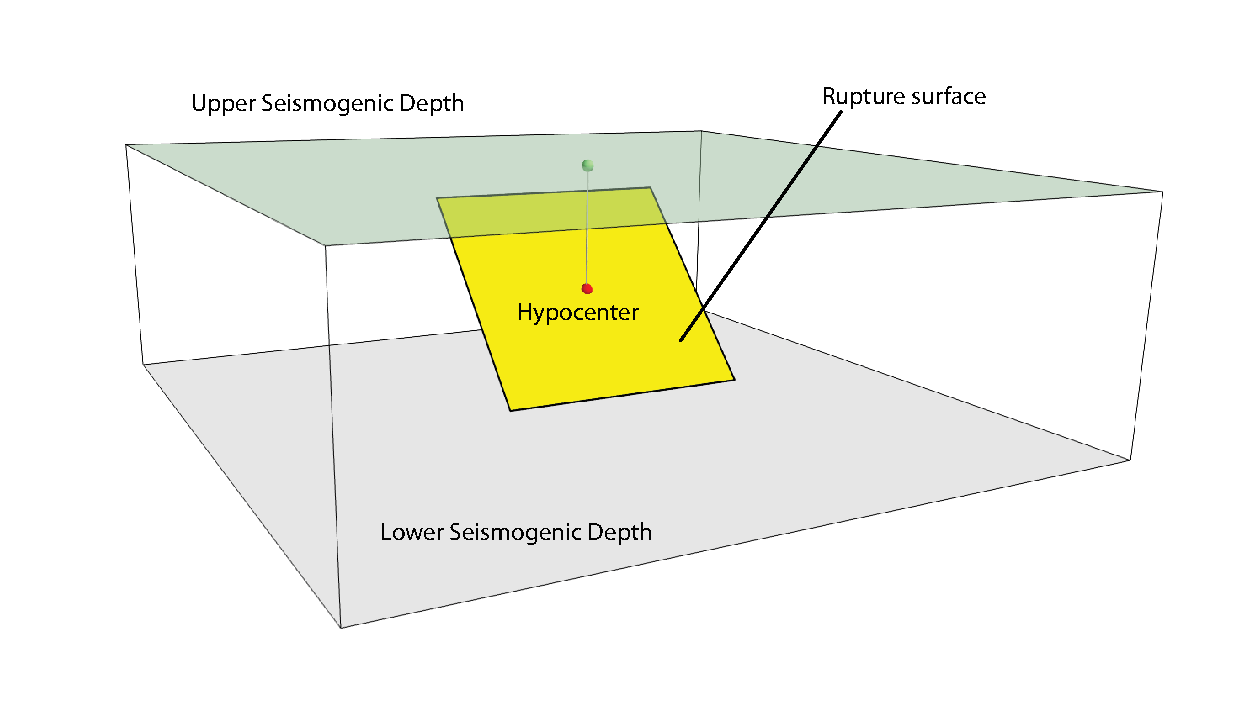
\includegraphics[width=10cm]{./figures/hazard/single_rupture.eps}
\caption{Single rupture}
\label{fig:single_rupture}
\end{figure}
% . . . . . . . . . . . . . . . . . . . . . . . . . . . . . . . . . . . < Figure
% ..............................................................................
Point source is the elemental source type adopted in the OpenQuake engine 
to model distributed seismicity. These are the basic assumptions used to 
generate finite ruptures with point sources:
\begin{itemize}
	\item ruptures have a rectangular shape
	\item rupture's hypocenter is located in the middle of the rupture
	\item ruptures are limited at the top and at the bottom by two planes 
	parallel to the topographic surface and placed at two characteristic 
	depths named upper and lower seismogenic depths, respectively.
\end{itemize} 
%
%  . . . . . . . . . . . . . . . . . . . . . . . . . . . . . . . . . . . . . . . 
\paragraph{Source data}
%
For each point source (i.e. grid node) the following parameters are requested
(Figure \ref{fig:single_rupture} shows some of the parameters described below, 
together with an example of rupture):
\begin{itemize}
\item The coordinates of the point (i.e. Longitude and Latitude in decimal 
    degrees)
\item The upper and lower seismogenic depths;
\item One \gls{mfd};
\item One magnitude-scaling relationship;
\item The rupture aspect ratio;
\item A distribution of nodal planes i.e. one (or several) instances 
    of the following set of parameters:
\begin{itemize}
    \item \gls{strike}
    \item \gls{dip}
    \item \gls{rake}
\end{itemize}
\item A magnitude independent depth distribution of hypocenters. 
\end{itemize}
%
Figure \ref{fig:point_source_multiple_ruptures} shows multiple ruptures 
of different magnitude centered on the single hypocentre allowed 
by this point source. Ruptures are created by conserving the area obtained
from magnitude through a magnitude-area scaling relatioship.
% ..............................................................................
% . . . . . . . . . . . . . . . . . . . . . . . . . . . . . . . . . . . > Figure
\begin{figure}[ht!]
\centering
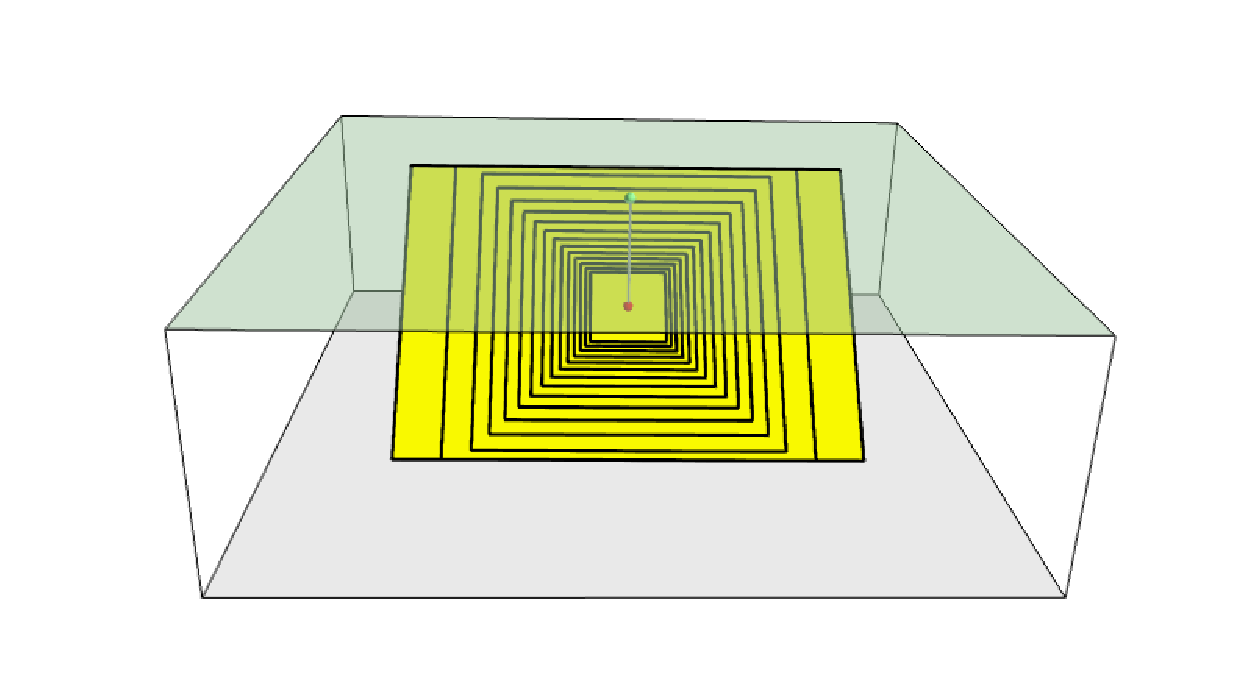
\includegraphics[width=10cm]{./figures/hazard/point_source_multiple_ruptures.ps}
\caption{Point source with multiple ruptures. Note the change in the aspect 
ratio once the rupture width fills the entire seismogenic layer.}
\label{fig:point_source_multiple_ruptures}
\end{figure}
% . . . . . . . . . . . . . . . . . . . . . . . . . . . . . . . . . . . < Figure
% ..............................................................................
Below we provide the excerpt of an .xml file used to describe the 
properties of a point source of a seismic source model.
\label{page:xml_point}
\begin{Verbatim}[frame=single, commandchars=\\\{\}, fontsize=\footnotesize,
    numbers=left, numbersep=2pt]
<pointSource id="1" name="point" tectonicRegion="Stable Continental Crust">
    <pointGeometry>
        <gml:Point>
            <gml:pos>-122.0 38.0</gml:pos>
        </gml:Point>
        <upperSeismoDepth>0.0</upperSeismoDepth>
        <lowerSeismoDepth>10.0</lowerSeismoDepth>
    </pointGeometry>
    <magScaleRel>WC1994</magScaleRel>
    <ruptAspectRatio>0.5</ruptAspectRatio>
    <truncGutenbergRichterMFD aValue="-3.5" bValue="1.0" minMag="5.0" 
			maxMag="6.5" />
    <nodalPlaneDist>
        <nodalPlane probability="0.3" strike="0.0" dip="90.0" rake="0.0" />
        <nodalPlane probability="0.7" strike="90.0" dip="45.0" rake="90.0" />
    </nodalPlaneDist>
    <hypoDepthDist>
        <hypoDepth probability="0.5" depth="4.0" />
        <hypoDepth probability="0.5" depth="8.0" />
    </hypoDepthDist>
</pointSource>
\end{Verbatim}
In this example, ruptures occur on two possible nodal planes and two 
hypocentral depths. Figure \ref{fig:point_source_ruptures} shows all 
the possible ruptures generated by the point source specified above.

% ..............................................................................
% . . . . . . . . . . . . . . . . . . . . . . . . . . . . . . . . . . . > Figure
\begin{figure}[!ht]
\centering
\includegraphics[width=10cm]{./figures/hazard/pointsrc_2strike_2hypodep.ps}
\caption{Ruptures produced by the source created using the information 
    in the example .xml file described at page \pageref{page:xml_point}.}
\label{fig:point_source_ruptures}
\end{figure}
% . . . . . . . . . . . . . . . . . . . . . . . . . . . . . . . . . . . < Figure
% ..............................................................................
%
% . . . . . . . . . . . . . . . . . . . . . . . . . . . . . . . . . . . . . . .
\subsubsection{Grid sources}
\label{hazard:seismic_source_types:gridSources}
\index{Source type!grid}
\index{Grid source|see{Source type}}
% 
A grid source is simply a collection of
point sources distributed over a regular grid (usually equally spaced in 
longitude and latitude).
%
In \gls{psha} a grid source can be considered a model alternative to area 
sources, since they both model distributed seismicity. 
%
Indeed, grid source is a typology used to reproduce a distributed 
seismicity process - usually involving events of low and intermediate 
magnitudes. 

Grid sources usually are computed using seismicity smoothing algorithms 
\citep[][amongst many others]{frankel1995,woo1996}. 
%
The use of this source type brings some advantages compared to area sources, 
since (1) it removes most of the unavoidable degree of subjectivity due to 
the definition of the geometries of the area sources and (2) it produces
a spatial pattern of seismicity that is usually closer to what observed in 
the reality. 
Nevertheless, some smoothing algorithms require an a-priori definition of 
some setup parameters that expose the calculation to a certain degree of 
partiality.

Grid sources are modelled in \gls{acr:oqe} simply as a set of point sources. 
%  . . . . . . . . . . . . . . . . . . . . . . . . . . . . . . . . . . . . . . . 
\subsubsection{Area sources}
\label{hazard:seismic_source_types:areaSources}
\index{Source type!area} 
\index{Area source|see{Source type}}
%
Area sources describe the seismicity occurring over wide areas where  
identification and characterization - i.e. the unambiguous definition 
of position, geometry and seismicity occurrence parameters - of single 
fault structures is difficult. 

From a computation standpoint area sources are comparable to grid sources.
The \gls{acr:oqe} using the source data parameters (see below)  
creates an equally spaced in distance grid of point sources where
each point has the same seismicity occurrence properties (i.e. rate
of events generated).

Below we provide a brief description of the parameters necessary to 
completely describe an area source:
%
%  . . . . . . . . . . . . . . . . . . . . . . . . . . . . . . . . . . . . . . . 
\paragraph{Source data}
\begin{itemize}
\item A polygon defining the external border of the area. 
The current version of OQ doesn't support the definition 
of internal borders
\item The upper and lower seismogenic depths;
\item One \gls{mfd};
\item One magnitude-scaling relationship;
\item The rupture aspect ratio;
\item A distribution of nodal planes i.e. one (or several) instances 
    of the following set of parameters:
\begin{itemize}
	\item strike
	\item dip
	\item rake
\end{itemize}
\item A magnitude independent depth distribution of hypocenters. 
\end{itemize}

Below we provide the exerpt of an .xml file used to describe the properties of
an area source of a seismic source model.
\begin{Verbatim}[frame=single, commandchars=\\\{\}, fontsize=\footnotesize,
numbers=left, numbersep=2pt]
<areaSource id="1" name="Quito" tectonicRegion="Active Shallow Crust">
    <areaGeometry>
        <gml:Polygon>
            <gml:exterior>
                <gml:LinearRing>
                    <gml:posList>
                     -122.5 37.5
                     -121.5 37.5
                     -121.5 38.5
                     -122.5 38.5
                    </gml:posList>
                </gml:LinearRing>
            </gml:exterior>
        </gml:Polygon>
        <upperSeismoDepth>0.0</upperSeismoDepth>
        <lowerSeismoDepth>10.0</lowerSeismoDepth>
    </areaGeometry>
    <magScaleRel>PeerMSR</magScaleRel>
    <ruptAspectRatio>1.5</ruptAspectRatio>
    <incrementalMFD minMag="6.55" binWidth="0.1">
        <occurRates>0.0010614989 8.8291627E-4 7.3437777E-4 6.108288E-4 
				5.080653E-4</occurRates>
    </incrementalMFD>
    <nodalPlaneDist>
        <nodalPlane probability="0.3" strike="0.0" dip="90.0" rake="0.0"/>
        <nodalPlane probability="0.7" strike="90.0" dip="45.0" rake="90.0"/>
    </nodalPlaneDist>
    <hypoDepthDist>
        <hypoDepth probability="0.5" depth="4.0" />
        <hypoDepth probability="0.5" depth="8.0" />
    </hypoDepthDist>
</areaSource>
\end{Verbatim}
The ruptures generated inside this area source follow to possible nodal 
planes and have hypocenters at two depths. 
%
%  . . . . . . . . . . . . . . . . . . . . . . . . . . . . . . . . . . . . . . .
\subsection{Fault source with floating ruptures}
%
Fault sources are classified according to the method adopted to 
distribute ruptures over the fault surface. Two are the option currently 
supported: 
\begin{itemize}
    \item Ruptures with a surface lower than the whole fault surface are 
        floated so as to cover as much as possible homogeneously the fault
        surface.
        This model is compatible with almost all the possible 
        magnitude-frequency distributions.
    \item Ruptures always fill the entire fault surface. This model is 
        compatible only with characteristic models (\`{a} la 
        \cite{schwartz1984}).
\end{itemize}
In this Section we discuss fault source types that support floating ruptures.
%
\subsubsection{Simple faults}
\index{Source type!fault!simple geometry} 
\index{Simple fault|see{Source type}}
%
Simple Faults are the most common source type used to model shallow 
faults; the ``simple'' adjective relates to the geometry description 
of the source which is basically obtained by projecting a trace 
(i.e. a polyline) along a characteristic dip direction. 

The parameters used to create an instance of this 
source type are described in the following paragraph.
%
%  .   .   .   .   .   .   .   .   .   .   .   .   .   .   .   .   .   .   .   . 
\paragraph{Source data}
%
\begin{itemize}
\item A \gls{faulttrace} (usually a polyline); 
\item A \gls{frequencymagnitudedistribution};
\item A representative value of the dip angle (specified following 
the Aki-Richards convention; see \citet{aki2002});
\item Rake angle (specified following the Aki-Richards convention; 
see \citet{aki2002}) 
\item Upper and lower depth values limiting the seismogenic interval; 
\end{itemize}
Below we provide the excerpt of an .xml file used to describe the 
properties of a simple fault source.
\begin{Verbatim}[frame=single, commandchars=\\\{\}, fontsize=\footnotesize,
    numbers=left, numbersep=2pt]
<simpleFaultSource id="1" name="Mount Diablo Thrust" 
		tectonicRegion="Active Shallow Crust">
    <simpleFaultGeometry>
        <gml:LineString>
            <gml:posList>
                -121.82290 37.73010
                -122.03880 37.87710
            </gml:posList>
        </gml:LineString>
        <dip>45.0</dip>
        <upperSeismoDepth>10.0</upperSeismoDepth>
        <lowerSeismoDepth>20.0</lowerSeismoDepth>
    </simpleFaultGeometry>
    <magScaleRel>WC1994</magScaleRel>
    <ruptAspectRatio>1.5</ruptAspectRatio>
    <incrementalMFD minMag="5.0" binWidth="0.1">
        <occurRates>0.0010614989 8.8291627E-4 7.3437777E-4 6.108288E-4 
				5.080653E-4</occurRates>
    </incrementalMFD>
    <rake>30.0</rake>
</simpleFaultSource>
\end{Verbatim}
%
%  . . . . . . . . . . . . . . . . . . . . . . . . . . . . . . . . . . . . . . .
\subsubsection{Complex faults}
\index{Source type!fault!complex geometry}
\index{Complex fault|see{Source type}}
%
Complex faults differ from simple fault just by the way the geometry of 
the fault surface is defined and, consequently by the way the fault 
surface is later created. 
The input parameters used to describe complex faults are, for the most 
part, the same used to describe the simple fault typology. 
In case of complex faults the dip angle is not requested while the fault
trace is substituted by two fault edges limiting at the top and bottom 
the fault surface. Additional curves lying over the fault surface can be 
specified to complement and refine the description of the fault surface 
geometry.
%
Usually, we use complex faults to model intraplate megathrust faults such 
as the big subduction structures active in the Pacific (Sumatra, South 
America, Japan).
\begin{Verbatim}[frame=single, commandchars=\\\{\}, fontsize=\footnotesize,
    numbers=left, numbersep=2pt]
<complexFaultSource id="1" name="Cascadia Megathrust" 
		tectonicRegion="Subduction Interface">
    <complexFaultGeometry>
        <faultTopEdge>
            <gml:LineString>
                <gml:posList>
                    -124.704  40.363  0.5493260E+01
                    -124.977  41.214  0.4988560E+01
                    -125.140  42.096  0.4897340E+01
                </gml:posList>
            </gml:LineString>
        </faultTopEdge>
        <intermediateEdge>
            <gml:LineString>
                <gml:posList>
                    -124.704  40.363  0.5593260E+01
                    -124.977  41.214  0.5088560E+01
                    -125.140  42.096  0.4997340E+01
                </gml:posList>
            </gml:LineString>
        </intermediateEdge>
        <intermediateEdge>
            <gml:LineString>
                <gml:posList>
                    -124.704  40.363  0.5693260E+01
                    -124.977  41.214  0.5188560E+01
                    -125.140  42.096  0.5097340E+01
                </gml:posList>
            </gml:LineString>
        </intermediateEdge>
        <faultBottomEdge>
            <gml:LineString>
                <gml:posList>
                    -123.829  40.347  0.2038490E+02
                    -124.137  41.218  0.1741390E+02
                    -124.252  42.115  0.1752740E+02
                </gml:posList>
            </gml:LineString>
        </faultBottomEdge>
    </complexFaultGeometry>
    <magScaleRel>WC1994</magScaleRel>
    <ruptAspectRatio>2.0</ruptAspectRatio>
    <truncGutenbergRichterMFD aValue="-3.5" bValue="1.0" minMag="5.0" 
			maxMag="6.5" />
    <rake>30.0</rake>
</complexFaultSource>
\end{Verbatim}
%
%  . . . . . . . . . . . . . . . . . . . . . . . . . . . . . . . . . . . . . . .
\subsection{Fault source types without floating ruptures}
\subsubsection{Characteristic faults}
\index{Source type!fault!characteristic}
\index{Characteristic fault|see{Source type}}

%
%  .   .   .   .   .   .   .   .   .   .   .   .   .   .   .   .   .   .   .   . 
\paragraph{Source data}

    The magnitude-frequency distributions currently supported by the
\gls{acr:oqe} are the following:

\begin{description}


\item[A discrete incremental magnitude-frequency distribution]

It is the simplest distribution supported. It is defined by the minimum value
of magnitude (representing the mid point of the first bin) and the bin width.
The distribution itself is simply a sequence of floats describing the annual
number of events for different bins. The maximum magnitude admitted by this
magnitude-frequency distribution is just the sum of the minimum magnitude and
the product of the bin width by the number annual rate values.

Below we provide an example of the xml that should be incorporated in a
seismic source description in order to define this \gls{acr:mfd}. An
additional example for this distribution can be also found at
page~\pageref{example_incremental_mfd}.

\begin{Verbatim}[frame=single, commandchars=\\\{\}, fontsize=\footnotesize]
<incrementalMFD minMag="5.05" binWidth="0.1">
    <occurRates>0.15 0.08 0.05 0.03 0.015</occurRates>
</incrementalMFD>
\end{Verbatim}

The magnitude-frequency distribution obtained with the above parameters is
represented in Figure~\ref{fig:evenly_discretized_mfd}.

\begin{figure}[!ht]
\centering
\includegraphics[width=12cm]{figures/hazard/ed_mfd.pdf}
\caption{Example of an incremental magnitude-frequency distribution.}
\label{fig:evenly_discretized_mfd}
\end{figure}



\item[A double truncated Gutenberg-Richter distribution]

This distribution is described by means of a minimum \texttt{minMag} and
maximum magnitude \texttt{maxMag} and by the $a$ and $b$ values of the
Gutenberg-Richter relationship.

The syntax of the xml used to describe this magnitude-frequency distribution
is rather compact as demonstrated in the following example:

\begin{Verbatim}[frame=single, commandchars=\\\{\}, fontsize=\footnotesize]
<truncGutenbergRichterMFD aValue="5.0" bValue="1.0" minMag="5.0"
        maxMag="6.0"/>
\end{Verbatim}

Figure~\ref{fig:dt_gr_mfd} shows the magnitude-frequency distribution
obtained using the parameters of the considered example.

\begin{figure}[!ht]
\centering
\includegraphics[width=12cm]{figures/hazard/dt_mfd.pdf}
\caption{Example of a double truncated Gutenberg-Richter magnitude-frequency
distribution.}
\label{fig:dt_gr_mfd}
\end{figure}



%\item[Characteristic earthquake model (\`{a} la \cite{youngs1985})]
%    In \citexear{youngs1995}, \citeauthor{youngs1995}
%\begin{Verbatim}[frame=single, commandchars=\\\{\}, fontsize=\footnotesize]
%    AA
%\end{Verbatim}

%\begin{figure}[!ht]
%\centering
%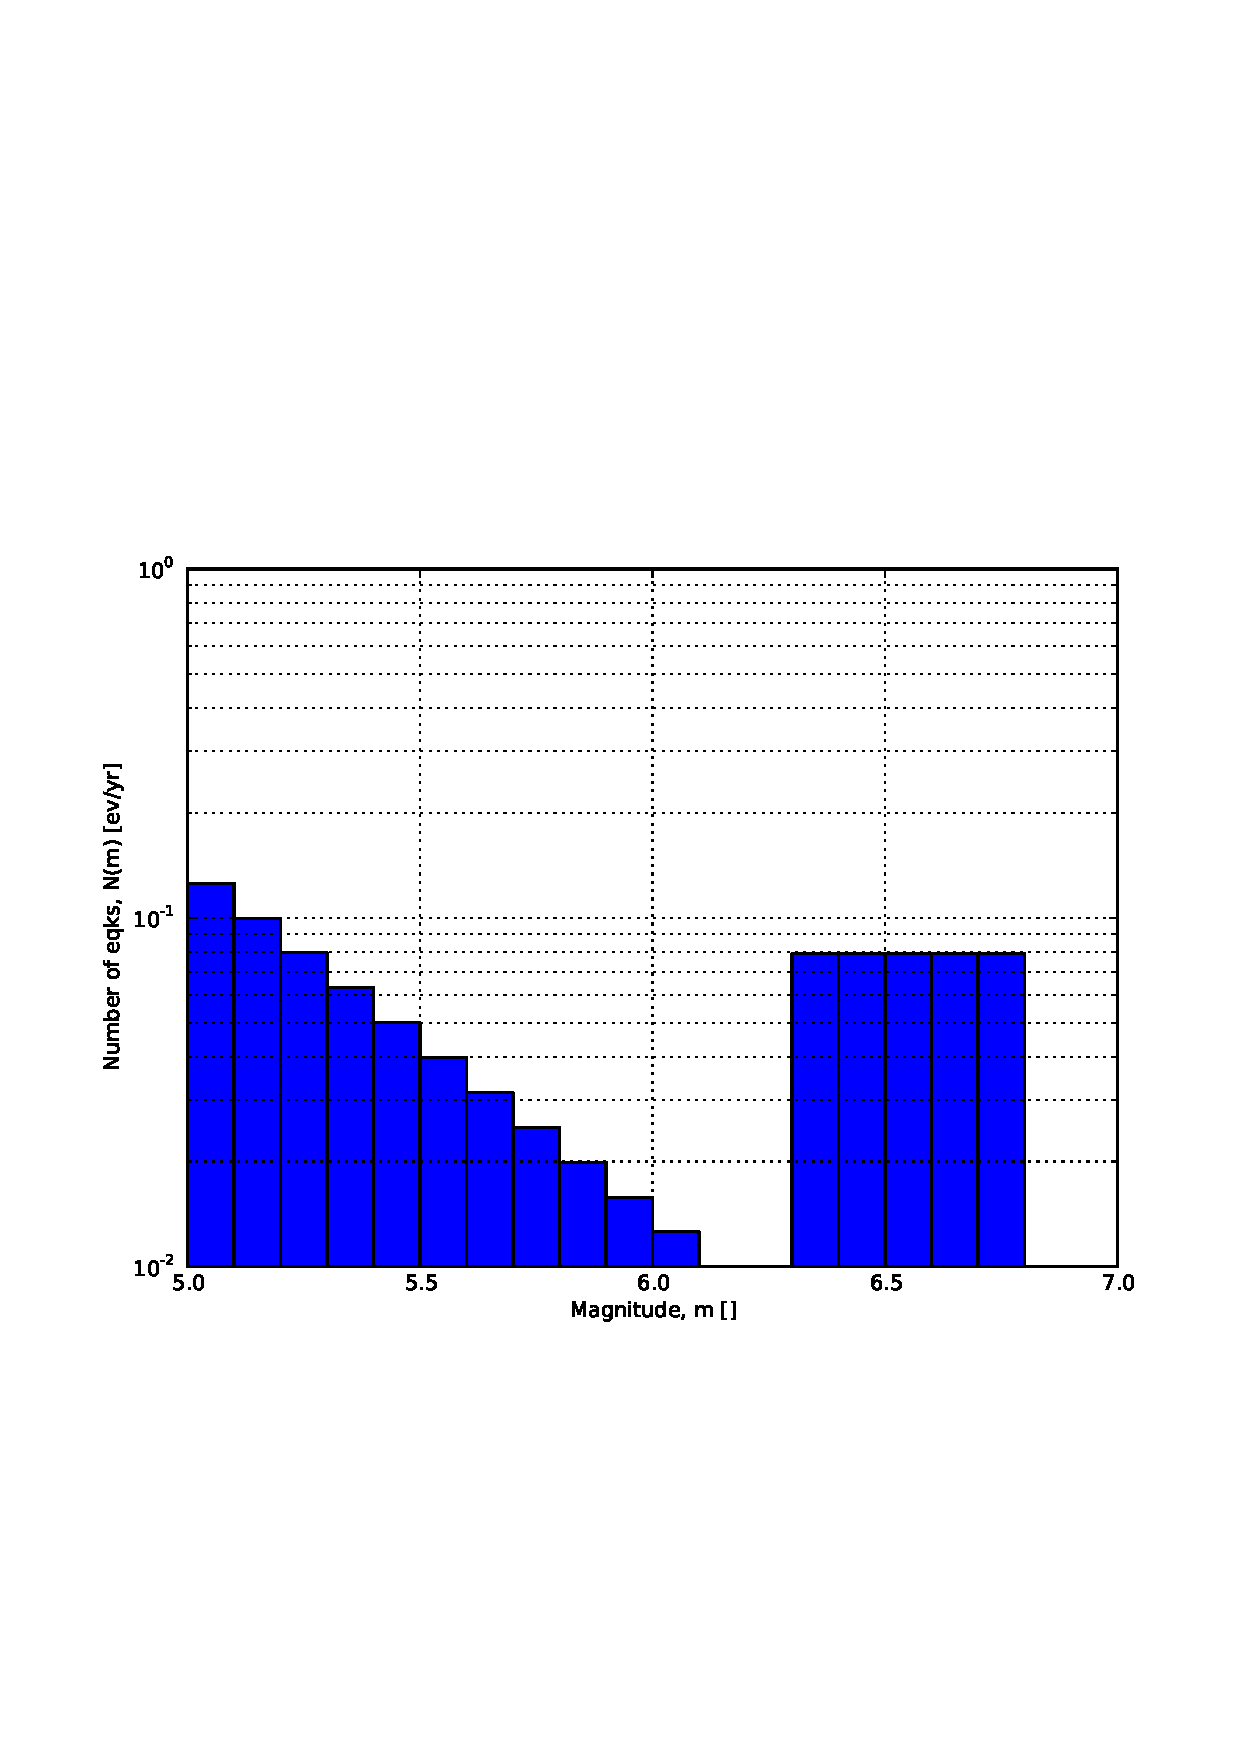
\includegraphics[width=12cm]{figures/hazard/yc_mfd.pdf}
%\caption{\cite{youngs1985} magnitude-frequency distribution.}
%\label{fig:yc_gr_mfd}
%\end{figure}

\end{description}

    % -----------------------------------------------------------------------------
\section{Calculation workflows}
\index{OpenQuake-engine!Hazard calculation workflows} 
% Three types of analysis
The hazard component of the OpenQuake-engine can compute seismic hazard 
using various approaches. 
%
Three types of analysis are currently supported:
\begin{itemize}
\item \textit{Classical Probabilistic Seismic Hazard Analysis (PSHA)}, 
allowing calculation of hazard curves and hazard maps following the 
classical integration procedure 
(\cite{cornell1968}, \citet{mcguire1976}) as formulated by \cite{field2003}.
%
\item \textit{Event-Based Probabilistic Seismic Hazard Analysis}, 
    allowing calculation of ground-motion fields from 
    stochastic event sets. Traditional results - 
    such as hazard curves - can be obtained by post-processing the 
    set of computed ground-motion fields.
\item \textit{\gls{acr:ssha}}, allowing the calculation of 
    ground motion fields from a single earthquake rupture scenario 
    taking into account ground-motion aleatory variability.
\end{itemize}
%
Each workflow has a modular structure, so that intermediate results 
can be exported and analyzed. 
Each calculator can be extended independently of the others so that 
additional calculation options and methodologies can be easily 
introduced, without affecting the overall calculation workflow. 
%
%  - - - - - - - - - - - - - - - - - - - - - - - - - - - - - - - - - - - - - - -
\subsection{Classical Probabilistic Seismic Hazard Analysis}
\index{OpenQuake-engine!Hazard calculation workflows!Classical PSHA} 
\label{section:classicalPSHA}
%
Input data for the classical \gls{acr:psha} consist of a PSHA input model
provided together with calculation settings. 

The main calculators used to perform this analysis are the following:
\begin{enumerate}
\item \emph{Logic Tree Processor} \hfill \\
The Logic Tree Processor (LTP) takes as an input the \gls{acr:psha} 
Input Model and creates a Seismic Source Model. The LTP uses the 
information in the Initial Seismic Source Models and  
the Seismic Source Logic Tree to create a Seismic Source Input
Model (i.e. a model describing geometry and activity rates of each 
source without any epistemic uncertainty). 
%
Following a procedure similar to the one just described the Logic Tree 
Processor creates a Ground Motion model (i.e. a data structure that 
associates to each tectonic region considered in the calculation a 
\gls{acr:gmpe}).
%
\item \emph{Earthquake Rupture Forecast Calculator} \hfill \\
The produced Seismic Source Input Model becomes an input information for 
the Earthquake Rupture Forecast (ERF) calculator which creates a list 
earthquake ruptures admitted by the source model, each one characterized
by a probability of occurrence over a specified time span.
\item \emph{Classical PSHA Calculator} \hfill \\
The classical PSHA calculator uses the ERF and the Ground Motion model 
to compute hazard curves on each site specified in the calculation settings.
\end{enumerate} 
%
%  - - - - - - - - - - - - - - - - - - - - - - - - - - - - - - - - - - - - - - -
\subsection{Event-Based Probabilistic Seismic Hazard Analysis}
\index{OpenQuake-engine!Hazard calculation workflows!Event-based PSHA} 
\label{section:event-basedPSHA}
Input data for the Event-Based PSHA - as in the case of the 
Classical \gls{acr:psha} calculator - consist of a PSHA Input Model 
and a set of calculation settings.
%
% ..............................................................................
% . . . . . . . . . . . . . . . . . . . . . . . . . . . . . . . . . . . > Figure
% \begin{figure}
% \centering
% \includegraphics[width=14cm]{figures/event_based_workflow.pdf}
% \caption{Workflow for event-based PSHA. Similar to the classical PSHA workflow 
% (Figure \ref{classical_psha_workflow}), an ERF is computed, which is then used 
% to generate a stochastic event set (representative of the seismic activity of 
% a region in a given time span). Each event is then utilized to calculate a 
% ground-motion field over a region of interest.}
% \label{event_based_workflow}
% \end{figure}
% . . . . . . . . . . . . . . . . . . . . . . . . . . . . . . . . . . . < Figure
% ..............................................................................
The main calculators  used to perform this analysis are:
\begin{enumerate}
%
\item \emph{Logic Tree Processor} \hfill \\
The Logic Tree Processor works in the same way described in 
the description of the Classical \gls{acr:psha} workflow 
(see section \ref{section:classicalPSHA} at page 
\pageref{section:classicalPSHA}).
%
\item \emph{Earthquake Rupture Forecast Calculator} \hfill \\ 
The Earthquake Rupture Forecast Calculator was already 
introduced in the description of the PSHA workflow (see section 
\ref{section:classicalPSHA} at page \pageref{section:classicalPSHA}).
%
\item \emph{Stochastic Event Set Calculator} \hfill \\
The Stochastic Event Set Calculator generates a collection of Stochastic 
event sets by sampling the ruptures contained in the ERF according to their 
probability of occurrence. 
%
A Stochastic Event Set (SES) thus represents a potential realisation of the 
seismicity (i.e. a list of ruptures) produced by the set of seismic sources 
considered in the analysis over the time span fixed for the 
calculation of hazard. 
%
\item \emph{Ground Motion Field Calculator} \hfill \\
The Ground Motion Field Calculator computes for each event contained in a 
Stochastic Event Set a realization of the geographic distribution of the 
shaking by taking into account the aleatory uncertainties in 
the ground-motion model. Eventually, the Ground Motion Field calculator 
can consider the spatial correlation of the ground-motion during the 
generation of the \gls{acr:gmf}.
%
\item \emph{Event-based PSHA Calculator} \hfill \\
The event-based PSHA calculator takes a (large) set of ground-motion 
fields representative of the possible shaking scenarios that the investigated
area can experience over a (long) time span and for each 
site computes the corresponding hazard curve. 
%
This procedure is computationally intensive and is not recommended for 
investigating the hazard over large areas. 
\end{enumerate}
%
%  - - - - - - - - - - - - - - - - - - - - - - - - - - - - - - - - - - - - - - -
\subsection{Scenario based Seismic Hazard Analysis}
\index{OpenQuake-engine!Hazard calculation workflows!Scenario-based SHA} 
\label{section:deterministicSHA}
In case of \gls{acr:ssha}, the input data consist of a single earthquake 
rupture model and a single ground-motion model. Using the Ground Motion Field 
Calculator, multiple realizations of ground shaking can be computed, each 
realization sampling the aleatory uncertainties in the ground-motion model.

The main calculators used to perform this analysis are:
\begin{enumerate}
\item \emph{Ground Motion Field Calculator} \hfill \\
The Ground Motion Field Calculator was already 
introduced during the description of the event based PSHA workflow (see 
section \ref{section:event-basedPSHA} at page \pageref{section:classicalPSHA}).
\end{enumerate}
% ..............................................................................
% . . . . . . . . . . . . . . . . . . . . . . . . . . . . . . . . . . . > Figure
% \begin{figure}[!hb]
% \centering
% \includegraphics[width=14cm]{figures/deterministic_workflow.pdf}
% \caption{Workflow for deterministic SHA. Given a rupture scenario model, 
% consisting of an earthquake rupture model, plus a GMPE, the ground-motion 
% field calculator can compute multiple ground-motion field realizations (by 
% taking into account GMPE aleatory uncertainties).}
% \label{deterministic_workflow}
% \end{figure}
% ..............................................................................
\cleardoublepage

\chapter{Using the hazard module}
	\label{chap:hazinp}
	This Chapter summarises the structure of the information necessary 
to define a PSHA input model to be used with the OpenQuake-engine.
% -----------------------------------------------------------------------------
% -----------------------------------------------------------------------------
\section{Input Data definition}
\label{sec:hazInputData}
Input data for probabilistic based seismic hazard analysis (Classical, 
Event based, Disaggregation, and UHS) are organised into:
\begin{itemize}
\item A general configuration file;
\item A file describing the Seismic Source System, that is the set of 
    initial source models and associated epistemic uncertainties needed 
    to model the seismic activity in the region of interest.
\item A file describing the Ground Motion System, that is the set of ground 
    motion prediction equations, per tectonic region type, needed to model 
    the ground motion shaking in the region of interest.
\end{itemize}
%
Figure \ref{fig:psha_input} summarises the structure of a PSHA input model
for the OpenQuake-engine and the relationships between the files.
% ..............................................................................
% . . . . . . . . . . . . . . . . . . . . . . . . . . . . . . . . . . . > Figure
\begin{figure}[!ht]
\centering
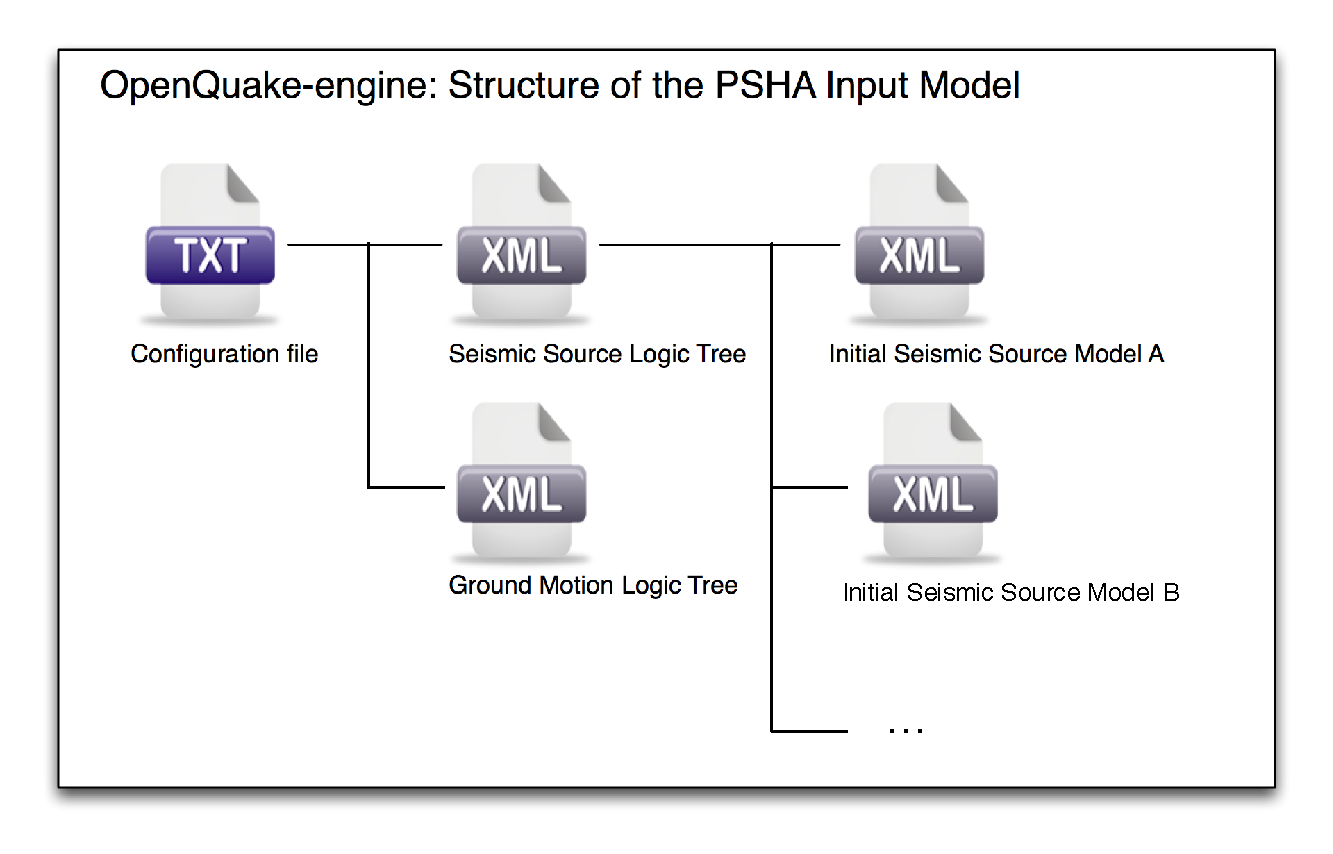
\includegraphics[width=14cm]{./figures/hazard/psha_input_structure.eps}
\caption{PSHA Input Model structure}
\label{fig:psha_input}
\end{figure}
% . . . . . . . . . . . . . . . . . . . . . . . . . . . . . . . . . . . < Figure
% ..............................................................................
% . . . . . . . . . . . . . . . . . . . . . . . . . . . . . . . . . . . . . . .
\subsection{Defining Logic Trees in the OpenQuake engine}
The main components of a logic tree structure in the OpenQuake engine are 
the following:
\begin{description}
    \item[branch]: the simplest component of a logic tree structure. 
    A branch represent an alternative 
    \item[branching set]: it groups a set of branches i.e. 
    alternative interpretation of a parameter or a model. This set of 
    uncertainties can be applied to the whole initial seismic source input 
    model or to a subset of seismic source data. The sum of the 
    weights/probabilities assigned to the set of branches 
    \item[branching level]: it's the largest container. It's not used in 
    modelling uncertainty, but it's useful in maintaining a logic and an 
    order in the structure of the logic tree as it's will be explained in 
    the following examples.
\end{description}

% . . . . . . . . . . . . . . . . . . . . . . . . . . . . . . . . . . . . . . .
\subsection{The Seismic Source System}
The Seismic Source System contains the models describing position, geometry 
and activity of seismic sources of engineering importance for a set of sites
as well as the possible epistemic uncertainties to be incorporated into the 
calculation of seismic hazard.
%
% . . . . . . . . . . . . . . . . . . . . . . . . . . . . . . . . . . . . . . .
\subsubsection{The Seismic Source Logic Tree}
The structure of the Seismic Source Logic Tree consists of at least one 
\gls{branchinglevel}. This branching level is the one used to define the 
\gls{initialseismicsourceinputmodel} (or a number of initial seismic source 
models, see Figure \ref{fig:psha_input}). 

The example provided below shows the simplest Seismic Source Logic Tree 
structure that can be defined in a \gls{pshainputmodel} for \gls{acr:oqe}. 
This consists of a logic tree with just one branching level containing 
one \gls{branchset} with one branch used to define the initial seismic source 
model (its weight will be equal to one).
\input{./oqum/hazard/verbatim/sslt_example.tex}

The optional branching levels will contain rules that modify parameters 
of the sources in the initial seismic source model so as to 
take into account the epistemic uncertainties. 

For example, if the principal epistemic uncertainties to be considered are
source geometry and maximum magnitude, the modeller can create a logic tree
structure with three initial seismic source models (each one exploring a 
different definition of the geometry of sources) and one branching level 
accounting for the epistemic uncertainty on the maximum magnitude.
 
Below we provide an example of such logic tree structure.
\input{./oqum/hazard/verbatim/sslt_example_simpleLT.tex}
Note that the uncertainty on the maximum magnitude is specified in terms 
of relative increments with respect to the initial maximum magnitude 
defined for each source in the initial seismic source models.
%
% . . . . . . . . . . . . . . . . . . . . . . . . . . . . . . . . . . . . . . .
\subsubsection{The Seismic Source Model}
\index{Input!Configuration file} 
The structure of the xml file representing the seismic source 
model corresponds to a list of sources, each one modelled using 
one out of the five typologies currently supported as demonstrated in 
the following schematic example.
\input{./oqum/hazard/verbatim/ssm_sample.tex}
%
% . . . . . . . . . . . . . . . . . . . . . . . . . . . . . . . . . . . . . . .
\subsection{The Ground Motion System}
\index{Input!Ground motion system} 
The Ground Motion System defines the models and possible epistemic 
uncertainties to be incorporated into the calculation of seismic hazard
and related to ground motion modelling.
%
% . . . . . . . . . . . . . . . . . . . . . . . . . . . . . . . . . . . . . . .
\subsubsection{The Ground Motion Logic Tree}
\index{Input!Ground motion logic tree} 
\label{ref:gmlt_example}
The structure of the \gls{groundmotionlogictree} consists of a list 
of ground motion prediction equations for each tectonic region used to
characterise the sources in the PSHA input model.

The example below shows a fairly simple \gls{groundmotionlogictree}. 
This logic tree assumes that all the sources in the PSHA input model 
belong to ``Active Shallow Crust'' and uses for calculation the 
\citet{chiou2008} \gls{acr:gmpe}.
\input{./oqum/hazard/verbatim/gmlt_example.tex}
%
% . . . . . . . . . . . . . . . . . . . . . . . . . . . . . . . . . . . . . . . 
% . . . . . . . . . . . . . . . . . . . . . . . . . . . . . . . . . . . . . . . 
\subsection{Configuration file}
\index{Input!Configuration file} 
\label{sec:conf_file}
The configuration file is the primary file controlling both the 
definition of the input model as well as parameters governing the 
calculation. We illustrate in the following different examples of 
the configuration file addressing different typologies of seismic 
hazard calculation.
\subsubsection{Calculation of a hazard map and hazard curves using 
    the classical PSHA methodology}
\label{sec:config_classical_PSHA}
%
In the following we describe the overall structure and the
most typical parameters of a configuration file to be used for the 
computation of a seismic hazard map using a classical PSHA methodology.
\begin{itemize}
\item \textbf{Calculation type and model info}
\begin{Verbatim}[frame=single, commandchars=\\\{\}, fontsize=\small,
    numbers=left, numbersep=2pt]
[general]
description = A demo OpenQuake-engine .ini file for classical PSHA
calculation_mode = classical
random_seed = 1024
\end{Verbatim}
In this section the user specifies the following parameters:
\begin{itemize}
    \item \texttt{description}: a parameter that can be used to designate 
        the model 
    \item \texttt{calculation\_mode}: it is used to set the kind 
        of calculation. In this case it corresponds to \texttt{classical}.
        We'll describe alternative options later on.
    \item \texttt{random\_seed}: is used to control the random generator 
        so that when montecarlo procedures are used calculations are 
        replicable (if the same \texttt{random\_seed} is used you get 
        exactly the same results).
\end{itemize}
%
\item \textbf{Geometry of the area (or the sites) where hazard is computed}
    \hfill \\
This section is used to specify where hazard will be computed. Two 
option are available. 

The first one consists on defining a polygon 
(usually a rectangle) and a distance (in km) used to discretize the 
polygon area. The polygon is defined by a list of longitude-latitude tuples.

An example is provided below.
\begin{Verbatim}[frame=single, commandchars=\\\{\}, fontsize=\small,
    firstnumber=5, numbers=left, numbersep=2pt]
[geometry]
region = 10.0 43.0, 12.0 43.0, 12.0 46.0, 10.0 46.0
\# km
region_grid_spacing = 10.0
\end{Verbatim}

The second option allows the definition of a number of sites where 
the hazard will be computed. An example is provided below.
\begin{Verbatim}[frame=single, commandchars=\\\{\}, fontsize=\small,
    firstnumber=5, numbers=left, numbersep=2pt]
[geometry]
sites = 10.0 43.0, 12.0 43.0, 12.0 46.0, 10.0 46.0


\end{Verbatim}
If the list of sites is too long the user can specify the name 
of a .csv file as it is shown below
\begin{Verbatim}[frame=single, commandchars=\\\{\}, fontsize=\small,
    firstnumber=5, numbers=left, numbersep=2pt]
[geometry]
sites\_csv = <name_of_the_csv_file>


\end{Verbatim}
The format of the csv file containing the list of sites 
is a sequence of points (one per row) specified in terms 
of the longitude, latitude tuple. An example is provided below,
\begin{Verbatim}[frame=single, commandchars=\\\{\}, fontsize=\small,
    firstnumber=1, numbers=left, numbersep=2pt]
179.0,90.0
178.0,89.0
177.0,88.0
\end{Verbatim}


%
\item \textbf{Logic tree sampling} \hfill \\
    The \gls{acr:oqe} provides two options for processing the whole 
    logic tree structure. The first option uses Montecarlo sampling;
    the user in this case specifies a number of realizations. 

    In the second option all the possible realizations are created. 
    Below we provide an example for the latter option.
    In this case we set the \texttt{number\-\_of\-\_logic\_tree\_samples}
    to 0. \gls{acr:oqe} will perform a complete enumeration of all 
    the possible paths from the roots to the leaves of the logic tree 
    structure. 
\begin{Verbatim}[frame=single, commandchars=\\\{\}, fontsize=\small,
    firstnumber=9, numbers=left, numbersep=2pt]
[logic_tree]
number_of_logic_tree_samples = 0
\end{Verbatim}
    If the seismic source logic tree and the ground motion
    logic tree do not contain epistemic uncertainties the engine will
    create a single PSHA input.
%
\item \textbf{Parameters controlling the construction of the earthquake 
    rupture forecast}
\begin{Verbatim}[frame=single, commandchars=\\\{\}, fontsize=\small,
    firstnumber=11, numbers=left, numbersep=2pt]
[erf]
# km
rupture_mesh_spacing = 5
width_of_mfd_bin = 0.1
# km
area_source_discretization = 10
\end{Verbatim}
This section of the configuration file is used to specify the 
level of discretization of the mesh representing faults, the grid
used to delineate the area sources and, the magnitude-frequency 
distribution. 
Note that the smaller is the mesh spacing (or the bin width) the larger 
are (1) the precision in the calculation and (2) the computation demand.
%
\item \textbf{Parameters describing site conditions}
\begin{Verbatim}[frame=single, commandchars=\\\{\}, fontsize=\small,
    firstnumber=17, numbers=left, numbersep=2pt]
[site_params]
reference_vs30_type = measured
reference_vs30_value = 760.0
reference_depth_to_2pt5km_per_sec = 5.0
reference_depth_to_1pt0km_per_sec = 100.0
\end{Verbatim}
In this section the user specifies local soil conditions. The simplest
solution is to define uniform site conditions (i.e. all the sites have 
the same characteristics). Alternatively it's possible to define 
spatially variable soil properties in a separate file; the engine will
then assign to each investigation location the values of the closest point
used to specify site conditions.
%
\begin{Verbatim}[frame=single, commandchars=\\\{\}, fontsize=\small,
    firstnumber=17, numbers=left, numbersep=2pt]
[site_params]
site_model_file = ../_site_model/site_model.xml



\end{Verbatim}
The file containing the site model has the following 
structure:
\begin{Verbatim}[frame=single, commandchars=\\\{\}, fontsize=\small]
<?xml version="1.0" encoding="utf-8"?>
<nrml xmlns:gml="http://www.opengis.net/gml"
      xmlns="http://openquake.org/xmlns/nrml/0.4">
    <siteModel>
        <site lon="10.0" lat="40.0" vs30="800.0" 
            vs30Type="inferred" 
            z1pt0="19.367196734" z2pt5="0.588625072259" />
        <site lon="10.1" lat="40.0" vs30="800.0" 
            vs30Type="inferred" 
            z1pt0="19.367196734" z2pt5="0.588625072259" />
        <site lon="10.2" lat="40.0" vs30="800.0" 
            vs30Type="inferred" 
            z1pt0="19.367196734" z2pt5="0.588625072259" />
        <site lon="10.3" lat="40.0" vs30="800.0" 
            vs30Type="inferred" 
            z1pt0="19.367196734" z2pt5="0.588625072259" />
        <site lon="10.4" lat="40.0" vs30="800.0" 
            vs30Type="inferred" 
            z1pt0="19.367196734" z2pt5="0.588625072259" />
        ...
    </siteModel>
</nrml>
\end{Verbatim}

%
\item \textbf{Calculation configuration}
\phantomsection
\label{sec:calculation_configuration}
\begin{Verbatim}[frame=single, commandchars=\\\{\}, fontsize=\small,
     firstnumber=22, numbers=left, numbersep=2pt]
[calculation]
source_model_logic_tree_file = source_model_logic_tree.xml
gsim_logic_tree_file = gmpe_logic_tree.xml
# years
investigation_time = 50.0
intensity_measure_types = PGA, SA(0.1)
intensity_measure_types_and_levels = \{"PGA": [0.005, ..., 2.13]\} 
truncation_level = 3
# km
maximum_distance = 200.0
\end{Verbatim}
This section of the \gls{acr:oqe} configuration file specifies the 
parameters that
are relevant for the calculation of hazard. These include the names of
the two files containing the Seismic Source System and the Ground 
Motion System, the duration of the time window used to compute the 
hazard, the ground motion intensity measure types and levels for 
which the probability of exceedence will be computed, the level of
truncation of the gaussian 
distribution of the logarithm of ground motion used in the calculation 
of hazard and the maximum integration distance (i.e. the distance within 
which sources will contribute to the computation of the hazard).
%
\item \textbf{Output}
\begin{Verbatim}[frame=single, commandchars=\\\{\}, fontsize=\small,
    firstnumber=32, numbers=left, numbersep=2pt]
[output]
export_dir = out/
# given the specified `intensity_measure_types_and_levels`
quantile_hazard_curves =
poes_hazard_maps = 0.1
\end{Verbatim}
The final section of the configuration file is the one that contains 
the parameters controlling the typology of output to be produced.
%
\end{itemize}
%
%\input{config_file_event_based.tex}
%

\subsubsection{Seismic hazard disaggregation}
%
In this section we describe the structure of the configutation 
file to be used to complete a seismic hazard disaggregation. 
Since only a few parts of the standard configuration file need to 
be changed we'll use the description given in Section 
\ref{sec:config_classical_PSHA} at page 
\pageref{sec:config_classical_PSHA} as a reference and we'll 
emphasize herein major differences.
%
\begin{itemize}
%
\item \textbf{Calculation type and model info}
\begin{Verbatim}[frame=single, commandchars=\\\{\}, fontsize=\small]
[general]
description = A demo .ini file for PSHA disaggregation
calculation_mode = disaggregation
random_seed = 1024
\end{Verbatim}
The calculation mode parameter in this case is set as 
\texttt{disaggregation}.
%
\item \textbf{Geometry of the area (or the sites) where hazard is computed}
\begin{Verbatim}[frame=single, commandchars=\\\{\}, fontsize=\small]
[geometry]
sites = 11.0 44.5


\end{Verbatim}
In the section it will be necessary to specify the geographic 
coordinates of the site (or the sites) where the disaggregation
will be performed.
%
\item \textbf{Disaggregation parameters}
\begin{Verbatim}[frame=single, commandchars=\\\{\}, fontsize=\small]
[disaggregation]
poes_disagg = 0.02, 0.1
mag_bin_width = 1.0
distance_bin_width = 25.0
# decimal degrees
coordinate_bin_width = 1.5
num_epsilon_bins = 3
\end{Verbatim}
With the disaggregation settings shown above we'll disaggregate the intensity
measure levels with 10\% and 2\% probability of exceedance using the
\texttt{in\-ves\-ti\-gation\_time} and the intensity measure types 
defined in the ``Calculation configuration'' section of the OpenQuake
configuration file (see page \pageref{sec:calculation_configuration}). 

The parameters \texttt{mag\_bin\_width},  \texttt{distance\_bin\_width},
\texttt{coordinate\_bin\_width} control the level of discretization of the
disaggregation matrix computed. \texttt{num\_epsilon\_bins} indicates the 
number of bins used to represent the contributions provided by different
values of epsilon.

If the user is interested in a specific type of disaggregation,
we suggest to use a very coarse gridding for the parameters that are 
not necessary. For example, if the user is interested in a magnitude-distance 
disaggregation, we suggest the use of very large value for the 
\texttt{coordinate\_\-bin\_\-width} and to set  \texttt{num\_epsilon\_bins}
equal to 1.
\end{itemize}

\subsubsection{Event based PSHA}
%
In the following we describe the sections of the logic tree that are 
specific for event based PSHA calculations (the remaining sections 
\begin{enumerate}
\item \textbf{Calculation type and model info}
    This part is almost identical to the corresponding one 
    describe in section \ref{sec:config_classical_PSHA}. Note
    the setting of the \texttt{calculation\_mode} parameter.
\begin{Verbatim}[frame=single, commandchars=\\\{\}, fontsize=\small,
    numbers=left, numbersep=2pt]
[general]
description = A demo OpenQuake-engine .ini file for classical PSHA
calculation_mode = event_based
random_seed = 1024
\end{Verbatim}
%
\item \textbf{Event based} \hfill \\
This is an additional part used to specify the number of stochastic 
event sets (each one representing a potential realisation of seismicity
during the \texttt{investigation\_time} specified in the 
\texttt{calculation\_configuration} part.
\begin{Verbatim}[frame=single, commandchars=\\\{\}, fontsize=\small]
[event_based_params]
ses_per_logic_tree_path = 5
ground_motion_correlation_model = JB2009
ground_motion_correlation_params = {"vs30_clustering": true}
\end{Verbatim}
%
\item \textbf{Output} \hfill \\
This part substitutes the \texttt{Output} part described in 
configuration file example descibed in section \ref{sec:config_classical_PSHA}
at page \pageref{sec:config_classical_PSHA}.
\begin{Verbatim}[frame=single, commandchars=\\\{\}, fontsize=\small]
[output]
export_dir = /tmp/xxx
complete_logic_tree_ses = true
complete_logic_tree_gmf = true
ground_motion_fields = true
# post-process ground motion fields into hazard curves,
# given the specified `intensity_measure_types_and_levels`
hazard_curves_from_gmfs = true
mean_hazard_curves = true
quantile_hazard_curves = 0.15, 0.5, 0.85
poes_hazard_maps = 0.1, 0.2
\end{Verbatim}
%
\end{enumerate}


\chapter{Hazard calculation and results provided}
	\label{chap:hazout}
	In this Chapter we provide a desciption of the main commands available
for running hazard with the \gls{acr:oqe} and the file formats used to 
represent the results of the analyses.

A general introduction to the use of OpenQuake is provided in Section 
\ref{sec:intro} at page \pageref{sec:intro}.
The reader is invited to consult this part before moving into
the details of this section.
% -----------------------------------------------------------------------------
\section{Running OpenQuake-engine for hazard calculations}
\index{Running OpenQuake!hazard} 
The execution of a hazard analysis using the OpenQuake-engine 
is straightforward. Below we provide an example of the simplest 
command that can be used to launch a hazard calculation which 
consists in the invocation of \texttt{openquake} together with 
the \texttt{--rh} option which stands for ``run hazard'' and 
the name of a configuration file (in the example below
it corresponds to \texttt{job.ini}):
\begin{Verbatim}[frame=single, commandchars=\\\{\}, fontsize=\small]
user@ubuntu:~$ openquake --rh job.ini
\end{Verbatim}

The amount of information prompted during the execution of the 
analysis is controlled by means of the \texttt{--log-level} flag 
as shown in the example below:
\begin{Verbatim}[frame=single, commandchars=\\\{\}, fontsize=\small]
user@ubuntu:~$ openquake --rh job.ini --log-level debug
\end{Verbatim}
In this example we ask the engine to provide an extensive amount
of information (usually not justified for a standard analysis). 
Alternative options are: \texttt{debug}, \texttt{info}, \texttt{progress},
\texttt{warn}, \texttt{error}, \texttt{critical}.
% -----------------------------------------------------------------------------
\subsection{Getting results}
There are two alternative ways to get results from the OpenQuake engine:
directly through the calculation or by exporting them from the 
internal \gls{acr:oqe} database once a calculation is completed. 

The first option is activated at the OpenQuake engine invocation by 
the flag \texttt{--exports xml} as shown in the example below
\begin{Verbatim}[frame=single, commandchars=\\\{\}, fontsize=\small]
user@ubuntu:~$ openquake --rh job.ini \textcolor{red}{--exports xml}
\end{Verbatim}

The second option, allows the user to export the computed results at 
their's disposal.
In order to get the list of results of the hazard calculations stored 
in the \gls{acr:oqe} database the user can utilize the following command:
\begin{Verbatim}[frame=single, commandchars=\\\{\}, fontsize=\small]
user@ubuntu:~$ openquake --lhc
\end{Verbatim}
The execution of this command will produce a list similar to the 
one provided below.
\begin{Verbatim}[frame=single, commandchars=\\\{\}, fontsize=\small]
user@ubuntu:~$ openquake --lhc
calc_id | num_jobs | latest_job_status | last_update | description
1 | 1 | failed | 2013-03-01 09:49:34  | Classical PSHA
2 | 1 | successful | 2013-03-01 09:49:56  | Classical PSHA
3 | 1 | failed | 2013-03-01 10:24:04  | Classical PSHA
4 | 1 | failed | 2013-03-01 10:28:16  | Classical PSHA
5 | 1 | failed | 2013-03-01 10:30:04  | Classical PSHA
6 | 1 | successful | 2013-03-01 10:31:53  | Classical PSHA
7 | 1 | failed | 2013-03-09 08:15:14  | Classical PSHA
8 | 1 | successful | 2013-03-09 08:18:04  | Classical PSHA
\end{Verbatim}
Subsequently the user can get the list of result stored for a specific 
hazard analysis
\begin{Verbatim}[frame=single, commandchars=\\\{\}, fontsize=\small]
user@ubuntu:~$ openquake --lho <calc_id>
id | output_type | name
3 | hazard_curve | hc-rlz-6
\end{Verbatim}
and finally extract an xml file for a specific hazard result 
\begin{Verbatim}[frame=single, commandchars=\\\{\}, fontsize=\small]
user@ubuntu:~$ openquake --eh <result_id> <path_to_the_output_folder>
\end{Verbatim}
% -----------------------------------------------------------------------------
% -----------------------------------------------------------------------------
\section{Description of outputs}
The results generated by the OpenQuake-engine are fundamentally 
of two distinct typologies differentiated by the presence (or 
absence) of epistemic uncertainty in the PSHA input model.

When epistemic uncertainty is incorporated into the 
calculation, the Open\-Quake\--engine calculators (e.g. Classical 
PSHA, Event Based PSHA, Disaggregation, UHS) produce a 
'distribution' of results (hazard curves, ground motion fields, 
disaggregation matrices, UHS) which is specular to the epistemic 
uncertainties introduced in the PSHA input model.

For each logic tree sample, results are computed and stored. 
Calculation of results statistics (mean, standard deviation, 
quantiles) are included in the hazard module of the 
OpenQuake-engine calculators (the only exception being 
disaggregation).
% - - - - - - - - - - - - - - - - - - - - - - - - - - - - - - - - - - - - - - -
\subsection{Output from Classical PSHA}
By default, the classical PSHA calculator computes and stores 
hazard curves for each logic tree sample.

When the PSHA input model doesn't contain epistemic uncertainties
the results will consist on a set of hazard curves (one for each 
investigated site). 
\begin{Verbatim}[frame=single, commandchars=\\\{\}, fontsize=\small]
user@ubuntu:~$ openquake --lho <calc_id>
id | output_type | name
\textcolor{red}{3 | hazard_curve | hc-rlz-6}
\end{Verbatim}

If \texttt{number\_of\_logic\_tree\_samples}, then N hazard curves 
files are generated:
\begin{Verbatim}[frame=single, commandchars=\\\{\}, fontsize=\small]
user@ubuntu:~$ openquake --lho <calc_id>
id | output_type | name
\textcolor{red}{5 | hazard_curve | hc-rlz-10}
\textcolor{red}{6 | hazard_curve | hc-rlz-7}
\textcolor{red}{7 | hazard_curve | hc-rlz-8}
\textcolor{red}{8 | hazard_curve | hc-rlz-9}
\textcolor{red}{9 | hazard_curve | hc-rlz-11}
\textcolor{red}{10 | hazard_curve | hc-rlz-12}
\end{Verbatim}
If we export from the database the hazard curves contained in 
one of the items above through this command below
\begin{Verbatim}[frame=single, commandchars=\\\{\}, fontsize=\small]
user@ubuntu:~$ openquake --eh <output_id> <output_directory>
\end{Verbatim}
we will obtain a nrml formatted file as represented in the example
above.
\begin{Verbatim}[frame=single, commandchars=\\\{\}, fontsize=\small]
<?xml version='1.0' encoding='UTF-8'?>
<nrml xmlns:gml="http://www.opengis.net/gml" 
      xmlns="http://openquake.org/xmlns/nrml/0.4">
  <hazardCurves \textcolor{red}{sourceModelTreePath="b1|b212"} 
      \textcolor{red}{gsimTreePath="b2" IMT="PGA" investigationTime="50.0"}>
    \textcolor{green}{<IMLs>0.005 0.007 0.0098 ... 1.09 1.52 2.13</IMLs>}
    <hazardCurve>
      <gml:Point>
      \textcolor{blue}{<gml:pos>10.0 45.0</gml:pos>}
      </gml:Point>
      <poEs>1.0 1.0 1.0 ... 0.000688359310522 0.0 0.0</poEs>
    </hazardCurve>
    ...
    <hazardCurve>
      <gml:Point>
      \textcolor{blue}{<gml:pos>lon lat</gml:pos>}
      </gml:Point>
      <poEs>poe1 poe2 ... poeN</poEs>
    </hazardCurve>
  </hazardCurves>
</nrml>
\end{Verbatim}
Notwithstanding the intuitiveness of this file, let's have a brief 
overview of the information included.

The overall content of this file is a list of hazard curves, one for
each investigated site, computed using a PSHA input model which 
can be either the single PSHA input model (if epistemic 
uncertainties are not accounted) or one possible realisation of 
the complete logic tree structure. 

The attributes of the \texttt{hazardCurves} element (see text in 
red in the example file above) specify the path used to create the 
seismic source model (\texttt{source\-Model\-TreePath}) and the ground
motion model (\texttt{gsim\-Tree\-Path}) plus the intensity measure type 
and the investigation time used to compute the probability of exceedance. 
The \texttt{IMLs} element (in green in the example above) contains the 
values of shaking for which OpenQuake computed the probability of 
exceedance in the investigation time.
For each site this file contains a \texttt{hazardCurve} element which 
includes the coordinates (longitude and latitude in decimal degrees) 
of the site and the values of the probability of exceedance for all the 
intensity measure levels specified in the \texttt{IMLs} element.

If together with hazard curves the calculation of hazard curves have 
been selected in the configuration file this is the kind of output
we should expect from OpenQuake:
\begin{Verbatim}[frame=single, commandchars=\\\{\}, fontsize=\small]
user@ubuntu:~$ openquake --lho <calc_id> 
id | output_type | name
17 | hazard_curve | hc-rlz-17
18 | hazard_curve | hc-rlz-18
19 | hazard_curve | hc-rlz-13
20 | hazard_curve | hc-rlz-14
21 | hazard_curve | hc-rlz-15
22 | hazard_curve | hc-rlz-16
23 | hazard_curve | quantile(0.5)-curves-PGA
24 | hazard_map | hazard-map(0.1)-PGA-rlz-17
25 | hazard_map | hazard-map(0.1)-PGA-rlz-18
26 | hazard_map | hazard-map(0.1)-PGA-rlz-13
27 | hazard_map | hazard-map(0.1)-PGA-rlz-14
28 | hazard_map | hazard-map(0.1)-PGA-rlz-15
29 | hazard_map | hazard-map(0.1)-PGA-rlz-16
30 | hazard_map | hazard-map(0.1)-PGA-quantile(0.5)
\end{Verbatim}


\clearpage
The Event Based PSHA calculator computes and stores stochastic event sets and
the corresponding ground motion fields.

This calculator can also produce hazard curves and hazard maps exactly in the
same way as done using the Classical PSHA calculator.

The inset below shows an example of the list of results provided by the
\gls{acr:oqe} at the end of an event-based PSHA calculation:

\begin{Verbatim}[frame=single, commandchars=\\\{\}, fontsize=\small]
user@ubuntu:~$ oq-engine --lho <calc_id>
id | output_type | name
\textcolor{red}{31 | ses | ses-coll-rlz-19}
\textcolor{green}{32 | gmf | gmf-rlz-19}
\textcolor{red}{33 | ses | ses-coll-rlz-20}
\textcolor{green}{34 | gmf | gmf-rlz-20}
35 | hazard_curve | hazard-curve-rlz-19-SA(0.1)
36 | hazard_curve | hazard-curve-rlz-20-SA(0.1)
37 | hazard_curve | hazard-curve-rlz-19-PGA
38 | hazard_curve | hazard-curve-rlz-20-PGA
39 | hazard_curve | mean curve for SA(0.1)
40 | hazard_curve | quantile curve (poe >= 0.15) for imt SA(0.1)
41 | hazard_curve | quantile curve (poe >= 0.50) for imt SA(0.1)
42 | hazard_curve | quantile curve (poe >= 0.85) for imt SA(0.1)
43 | hazard_curve | mean curve for PGA
44 | hazard_curve | quantile curve (poe >= 0.15) for imt PGA
45 | hazard_curve | quantile curve (poe >= 0.50) for imt PGA
46 | hazard_curve | quantile curve (poe >= 0.85) for imt PGA
\end{Verbatim}

This list in the inset above contains two sets of stochastic events (in red)
and two sets of ground motion fields (in blue).

The whole group of stochastic event set and ground motion fields can be
exported immediately using the results with \texttt{id} 35 and 25, respectively.

Below is an example showing a nrml file containing a collection of stochastic
event sets (2 ruptures):

\input{oqum/hazard/verbatim/output_ses}

The text in red shows the part which describes the id of the generated
stochastic event set and the investigation time covered.

The text in green emphasises the portion of the text used to describe a
rupture. The information provided describes entirely the geometry of the rupture as well as its rupturing properties (e.g. rake, magnitude). The rupture ID is a string that represents each rupture uniquely (including the case where the same rupture is sampled multiple times). The exact format may be subject to change from time-to-time; however, the ID will usually contain information regarding the specific logic tree branch sample (realisation), the stochastic event set counter, the ID of the source from which the rupture was samples and a unique number indicating the rupture identifier within the earthquake rupture forecast of the specific source.

This is an example of a nrml file containing one ground motion field:

\input{oqum/hazard/verbatim/output_gmf}

\section{Output from Disaggregation}
The \gls{acr:oqe} output of a disaggregation analysis  
corresponds to the combination of a hazard curve and a multidimensional 
matrix containing the results of the disaggregation.

The example below shows the list of disaggregation results obtained 
for four logic tree realisations. 
%
For each realisation, disaggregation has been completed for two  
intensity measure levels corresponding to different probabilities of 
exceedence in the specified \texttt{investigation time}.
\begin{Verbatim}[frame=single, commandchars=\\\{\}]
user@ubuntu:~$ openquake --lho <calc_id> 
id | output_type | name
19 | hazard_curve | hc-rlz-3
20 | hazard_curve | hc-rlz-3
21 | hazard_curve | hc-rlz-4
22 | hazard_curve | hc-rlz-4
23 | disagg_matrix | disagg(0.02)-rlz-3-SA(0.025)-POINT(10.1 40.1)
24 | disagg_matrix | disagg(0.1)-rlz-3-SA(0.025)-POINT(10.1 40.1)
25 | disagg_matrix | disagg(0.02)-rlz-3-PGA-POINT(10.1 40.1)
26 | disagg_matrix | disagg(0.1)-rlz-3-PGA-POINT(10.1 40.1)
27 | disagg_matrix | disagg(0.02)-rlz-4-SA(0.025)-POINT(10.1 40.1)
28 | disagg_matrix | disagg(0.1)-rlz-4-SA(0.025)-POINT(10.1 40.1)
29 | disagg_matrix | disagg(0.02)-rlz-4-PGA-POINT(10.1 40.1)
30 | disagg_matrix | disagg(0.1)-rlz-4-PGA-POINT(10.1 40.1)
\end{Verbatim}

In the following inset we show an example of the nrml file 
used to represent the different disaggregation matrices (highlighted 
in red) produced by OpenQuake-engine.
%
\begin{Verbatim}[frame=single, commandchars=\\\{\}, fontsize=\small]
<?xml version='2.0' encoding='UTF-8'?>
<nrml xmlns:gml="http://www.opengis.net/gml" 
      xmlns="http://openquake.org/xmlns/nrml/0.4">
  <disaggMatrices sourceModelTreePath="b1" gsimTreePath="b1" IMT="PGA" 
        investigationTime="50.0" lon="10.1" lat="40.1" 
        magBinEdges="5.0, 6.0, 7.0, 8.0" 
        distBinEdges="0.0, 25.0, 50.0, 75.0, 100.0" 
        lonBinEdges="9.0, 10.5, 12.0" 
        latBinEdges="39.0, 40.5" 
        epsBinEdges="-3.0, -1.0, 1.0, 3.0" 
        tectonicRegionTypes="Active Shallow Crust">
\textcolor{red}{    <disaggMatrix type="Mag" dims="3" poE="0.1" }
\textcolor{red}{            iml="0.033424622602">}
      <prob index="0" value="0.987374744394"/>
      <prob index="1" value="0.704295394366"/>
      <prob index="2" value="0.0802318409498"/>
\textcolor{red}{    </disaggMatrix>}
\textcolor{red}{    <disaggMatrix type="Dist" dims="4" poE="0.1" }
\textcolor{red}{            iml="0.033424622602">}
      <prob index="0" value="0.700851969171"/>
      <prob index="1" value="0.936680387051"/>
      <prob index="2" value="0.761883595568"/>
      <prob index="3" value="0.238687565571"/>
\textcolor{red}{    </disaggMatrix>}
\textcolor{red}{    <disaggMatrix type="TRT" dims="1" poE="0.1" }
\textcolor{red}{            iml="0.033424622602">}
      <prob index="0" value="0.996566187011"/>
\textcolor{red}{    </disaggMatrix>}
\textcolor{red}{    <disaggMatrix type="Mag,Dist" dims="3,4" poE="0.1" }
\textcolor{red}{            iml="0.033424622602">}
      <prob index="2,3" value="0.0"/>
\textcolor{red}{    </disaggMatrix>}
\textcolor{red}{    <disaggMatrix type="Mag,Dist,Eps" dims="3,4,3" poE="0.1" }
\textcolor{red}{            iml="0.033424622602">}
      <prob index="0,0,0" value="0.0785857271425"/>
      ...
\textcolor{red}{    </disaggMatrix>}
\textcolor{red}{    <disaggMatrix type="Lon,Lat" dims="2,1" poE="0.1"}
\textcolor{red}{            iml="0.033424622602">}
      <prob index="0,0" value="0.996566187011"/>
      <prob index="1,0" value="0.0"/>
\textcolor{red}{    </disaggMatrix>}
\textcolor{red}{    <disaggMatrix type="Mag,Lon,Lat" dims="3,2,1" poE="0.1"} 
\textcolor{red}{            iml="0.033424622602">}
      <prob index="0,0,0" value="0.987374744394"/>
      <prob index="0,1,0" value="0.0"/>
      <prob index="1,0,0" value="0.704295394366"/>
      <prob index="1,1,0" value="0.0"/>
      <prob index="2,0,0" value="0.0802318409498"/>
      <prob index="2,1,0" value="0.0"/>
\textcolor{red}{    </disaggMatrix>}
\textcolor{red}{    <disaggMatrix type="Lon,Lat,TRT" dims="2,1,1" poE="0.1"} 
\textcolor{red}{            iml="0.033424622602">}
      <prob index="0,0,0" value="0.996566187011"/>
      <prob index="1,0,0" value="0.0"/>
\textcolor{red}{    </disaggMatrix>}
  </disaggMatrices>
</nrml>

\end{Verbatim}
%\caption{Hazard map: nrml sample file}
%\label{vrb:disaggr}
%\end{nrmlsmp}



\chapter{Demonstrative examples}
	\label{chap:hazdemo}
	% -----------------------------------------------------------------------------
\section{OpenQuake Hazard Demos}
With the \gls{acr:oqe} installation a number of demos are provided showing practical examples
of input and configuration files definition for different use cases.
The following demos illustrate how to use \gls{acr:oqe} for various seismic hazard analysis:
\begin{itemize}
\item PointSourceClassicalPSHA
\item AreaSourceClassicalPSHA
\item SimpleFaultSourceClassicalPSHA
\item ComplexFaultSourceClassicalPSHA
\item CharacteristicFaultSourceCase1ClassicalPSHA
\item CharacteristicFaultSourceCase2ClassicalPSHA
\item CharacteristicFaultSourceCase3ClassicalPSHA
\item LogicTreeCase1ClassicalPSHA
\item LogicTreeCase2ClassicalPSHA
\item LogicTreeCase3ClassicalPSHA
\item EventBasedPSHA
\item Disaggregation
\end{itemize}

\subsection{Classical PSHA Demos}
A number of demos have been designed to show how to perform a classical PSHA calculation using the different available
source typologies and how to define non-trivial logic trees. It should be noted that the input files that will be illustrated are valid
not only for a classical PSHA calculation but also for event based and disaggregation analysis.\\

\subsubsection{Classical PSHA with different source typologies}
All the classical PSHA demos illustrating the different source typologies (all demos but the ones about Logic Tree definition)
share the following GSIM logic tree file:
\begin{Verbatim}[frame=single, commandchars=\\\{\}, fontsize=\normalsize]
<?xml version="1.0" encoding="UTF-8"?>

<nrml xmlns:gml="http://www.opengis.net/gml"
      xmlns="http://openquake.org/xmlns/nrml/0.4">
    <logicTree logicTreeID='lt1'>

        <logicTreeBranchingLevel branchingLevelID="bl1">
            <logicTreeBranchSet
               uncertaintyType="gmpeModel"
               applyToTectonicRegionType="Active Shallow Crust"
               branchSetID="bs1">

                <logicTreeBranch branchID="b1">
                     <uncertaintyModel>
                        BooreAtkinson2008
                     </uncertaintyModel>
                     <uncertaintyWeight>1.0</uncertaintyWeight>
                </logicTreeBranch>

            </logicTreeBranchSet>
        </logicTreeBranchingLevel>

    </logicTree>
</nrml>
\end{Verbatim}
Each source in the source model file is defined as belonging to \texttt{Active Shallow Crust}, and therefore the GSIM Logic Tree file
defines for simplicity a single GMPE (Boore and Atkinson 2008) which is associated to an \texttt{Active Shallow Crust} tectonic region type.\\
The configuration file is defined to compute hazard curves for several intensity measure types (PGV, PGA and Spectral
acceleration at different periods), hazard maps and uniform hazard spectra for different probabilities of exceedance:
\begin{Verbatim}[frame=single, commandchars=\\\{\}, fontsize=\normalsize]
[general]

description = ...
calculation_mode = classical
random_seed = 23

[geometry]

region = ...
region_grid_spacing = 5.0

[logic_tree]

number_of_logic_tree_samples = 0

[erf]

rupture_mesh_spacing = 2
width_of_mfd_bin = 0.1
area_source_discretization = 5.0

[site_params]

reference_vs30_type = measured
reference_vs30_value = 600.0
reference_depth_to_2pt5km_per_sec = 5.0
reference_depth_to_1pt0km_per_sec = 100.0

[calculation]

source_model_logic_tree_file = source_model_logic_tree.xml
gsim_logic_tree_file = gmpe_logic_tree.xml
investigation_time = 50.0
intensity_measure_types_and_levels =\{
"PGV": [2, 4, 6 ,8, 10, ...], 
"PGA": [0.005, 0.007, ...], 
"SA(0.025)": [...], 
"SA(0.05)": [...],
"SA(0.1)": [...], 
"SA(0.2)": [...], 
"SA(0.5)": [...], 
"SA(1.0)": [...],
"SA(2.0)": [...]\}
truncation_level = 3
maximum_distance = 200.0

[output]

export_dir = ...
mean_hazard_curves = false
quantile_hazard_curves =
hazard_maps = true
uniform_hazard_spectra = true
poes = 0.1 0.02
\end{Verbatim}
Hazard maps for the different demos are show in figure \ref{fig:hazard_maps1} and \ref{fig:hazard_maps2}.

\begin{figure} 
\centering 
\subcaptionbox{}
{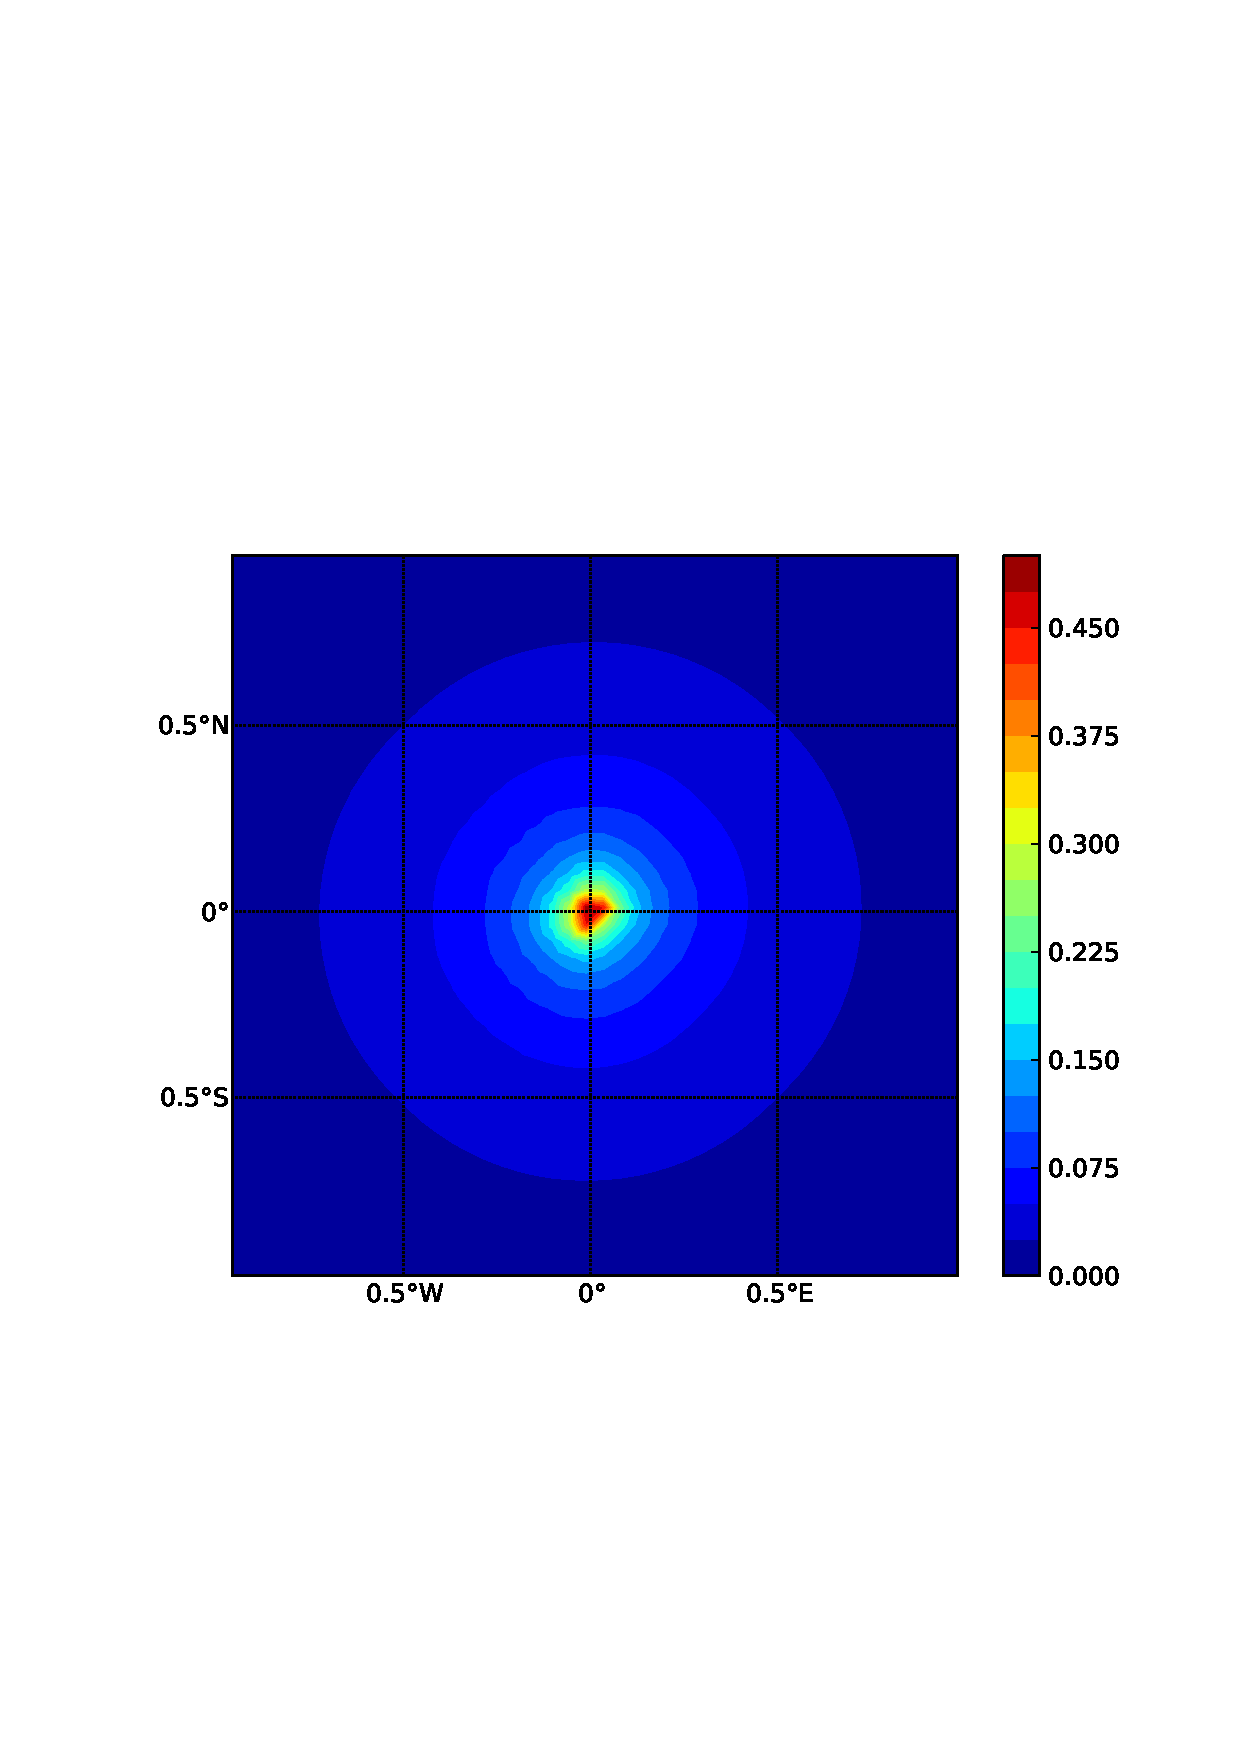
\includegraphics[width=7cm]{./figures/hazard/point.pdf}} 
\subcaptionbox{}
{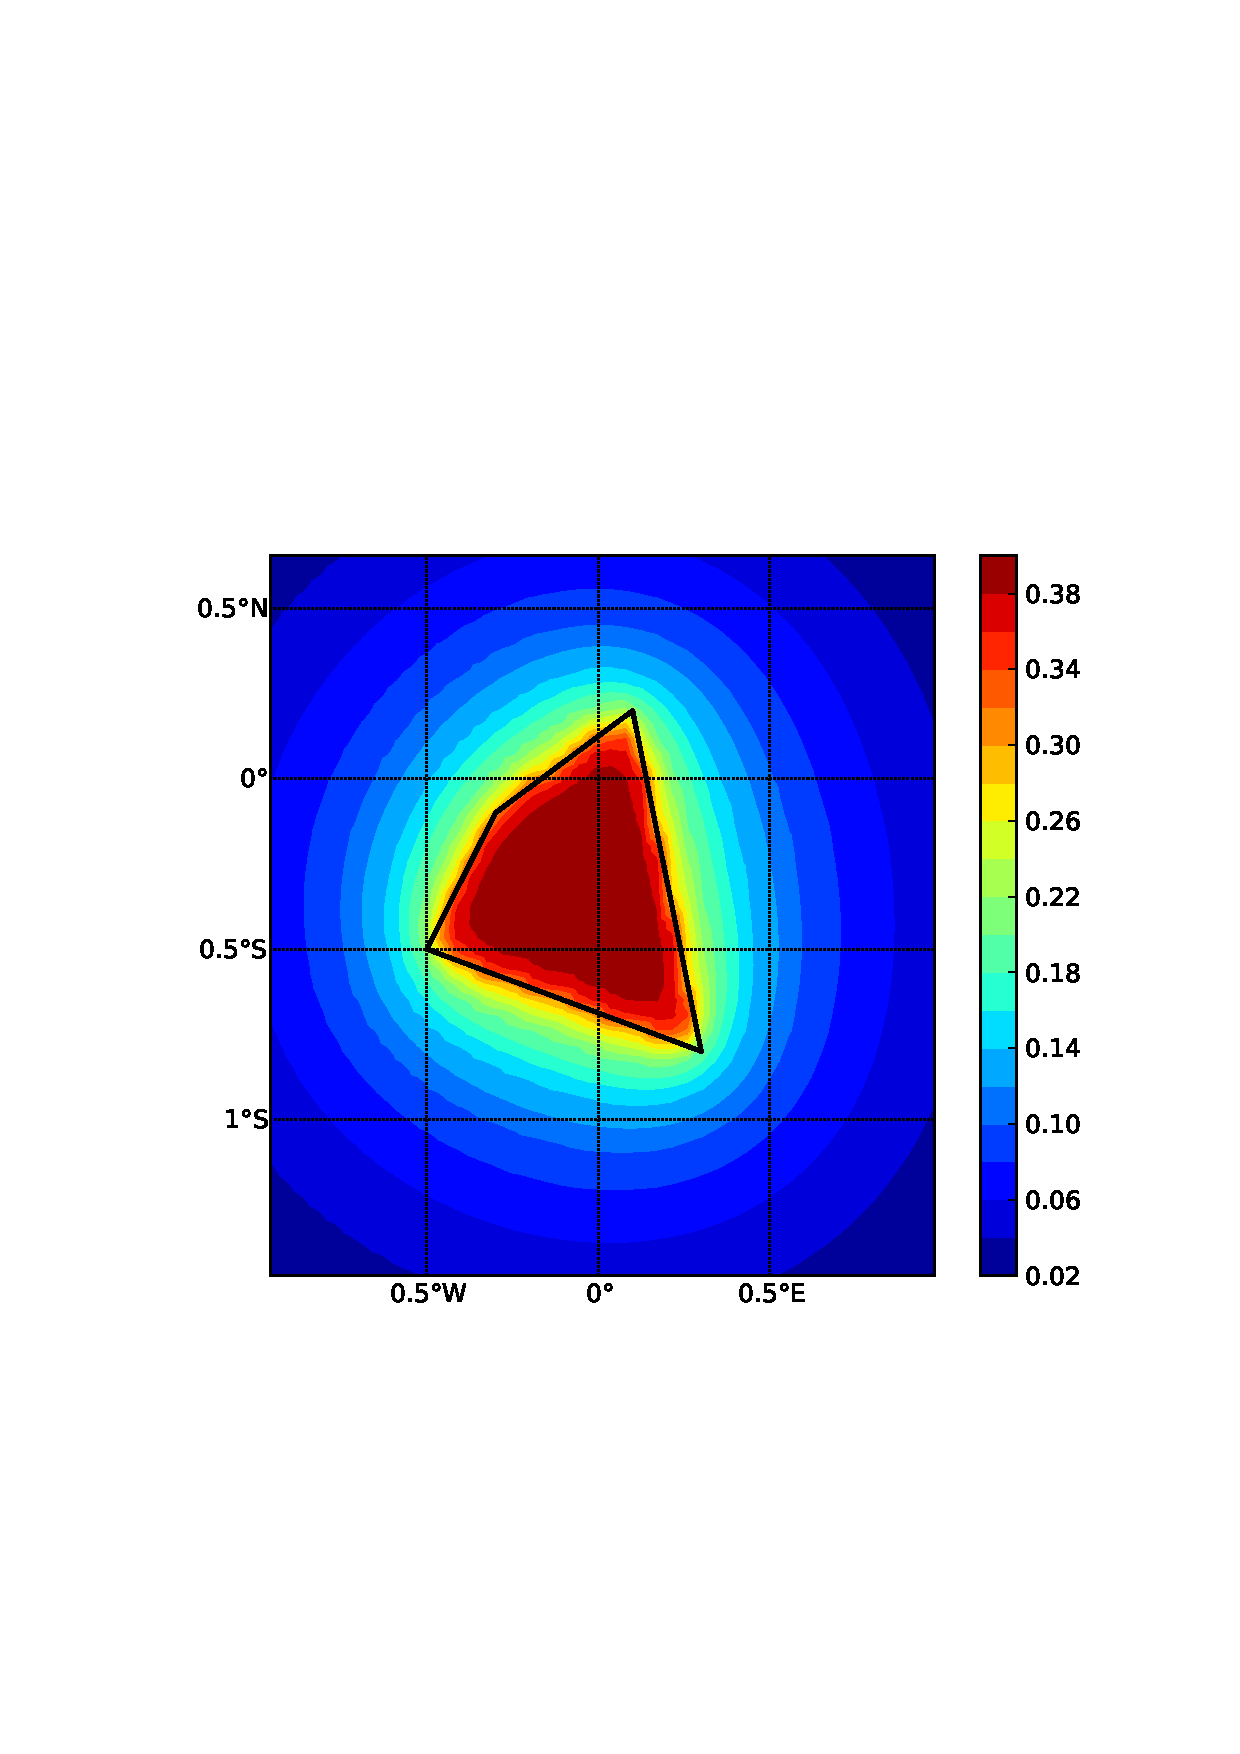
\includegraphics[width=7cm]{./figures/hazard/area.pdf}} 
\subcaptionbox{}
{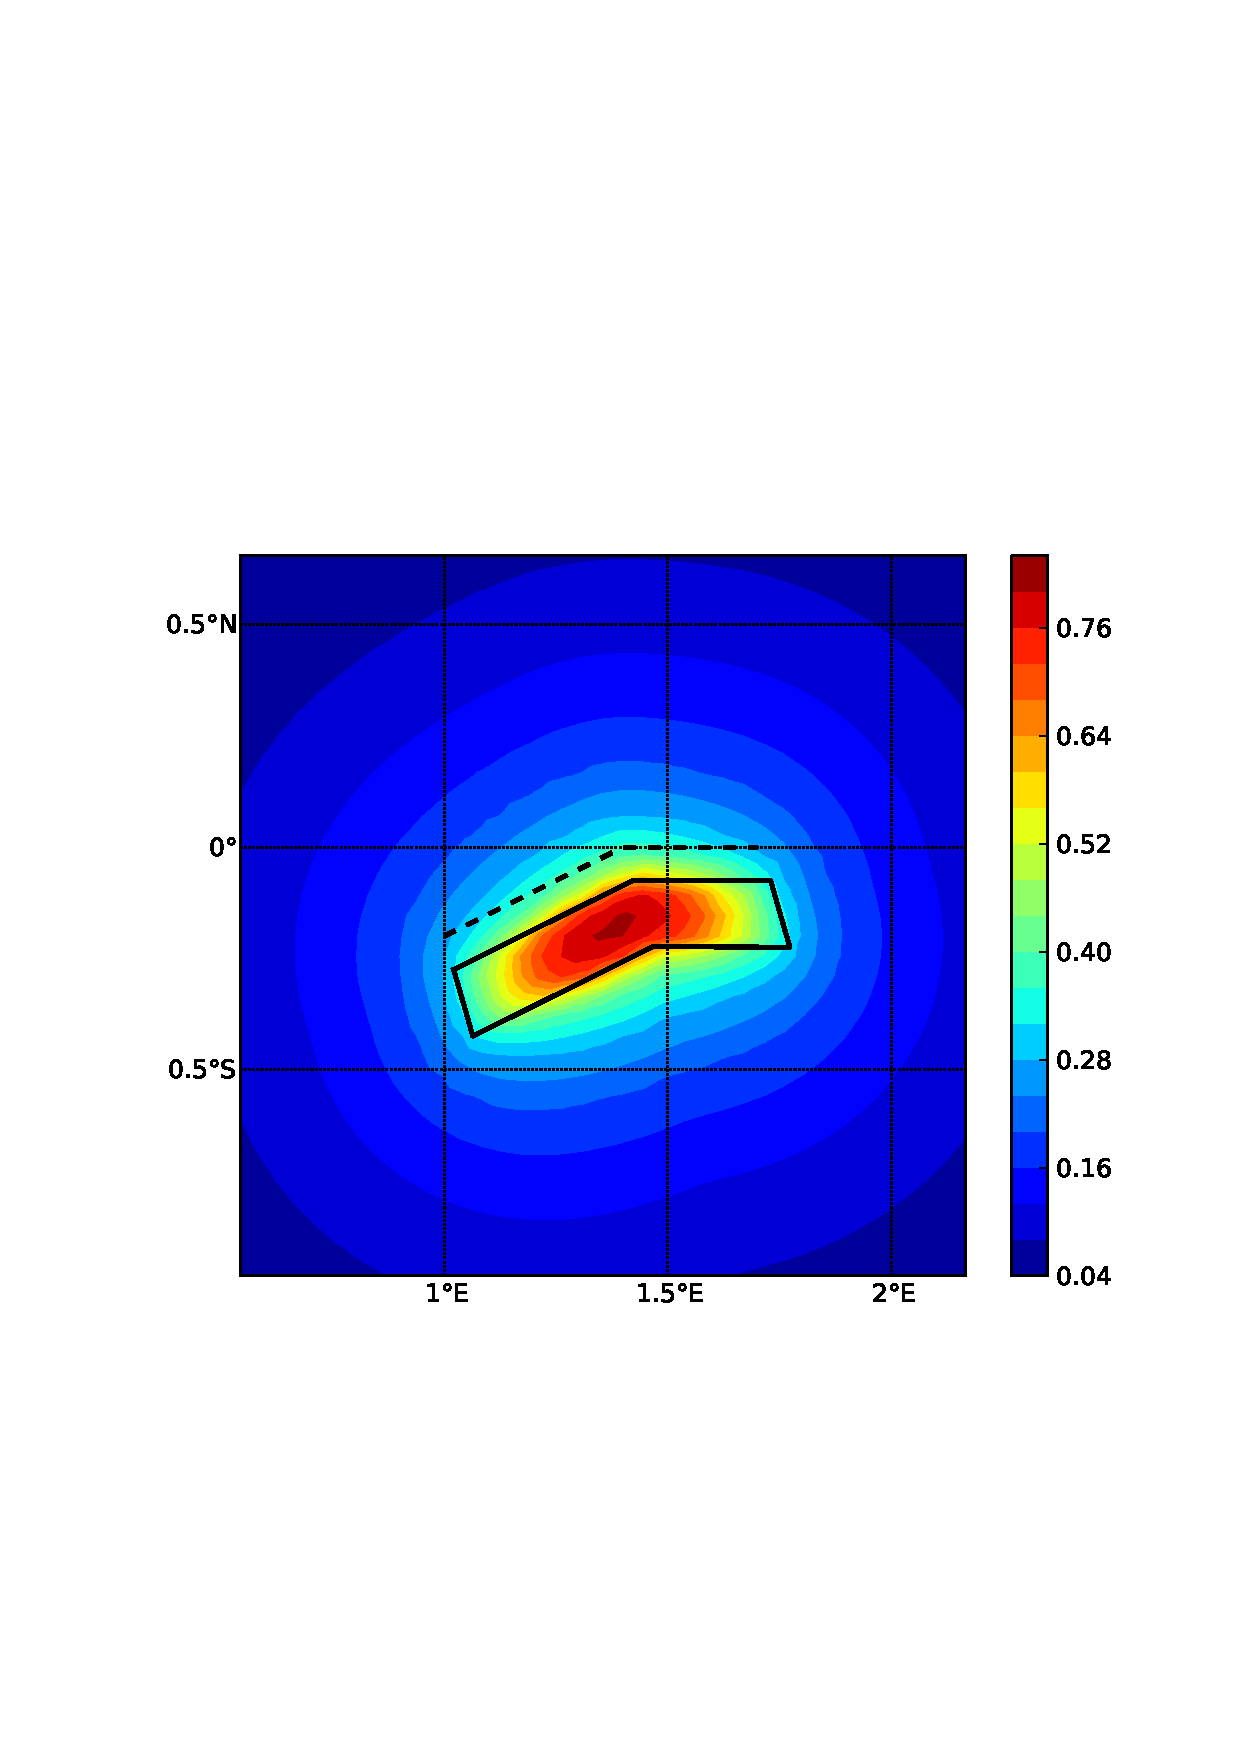
\includegraphics[width=7cm]{./figures/hazard/simple_fault.pdf}} 
\subcaptionbox{}
{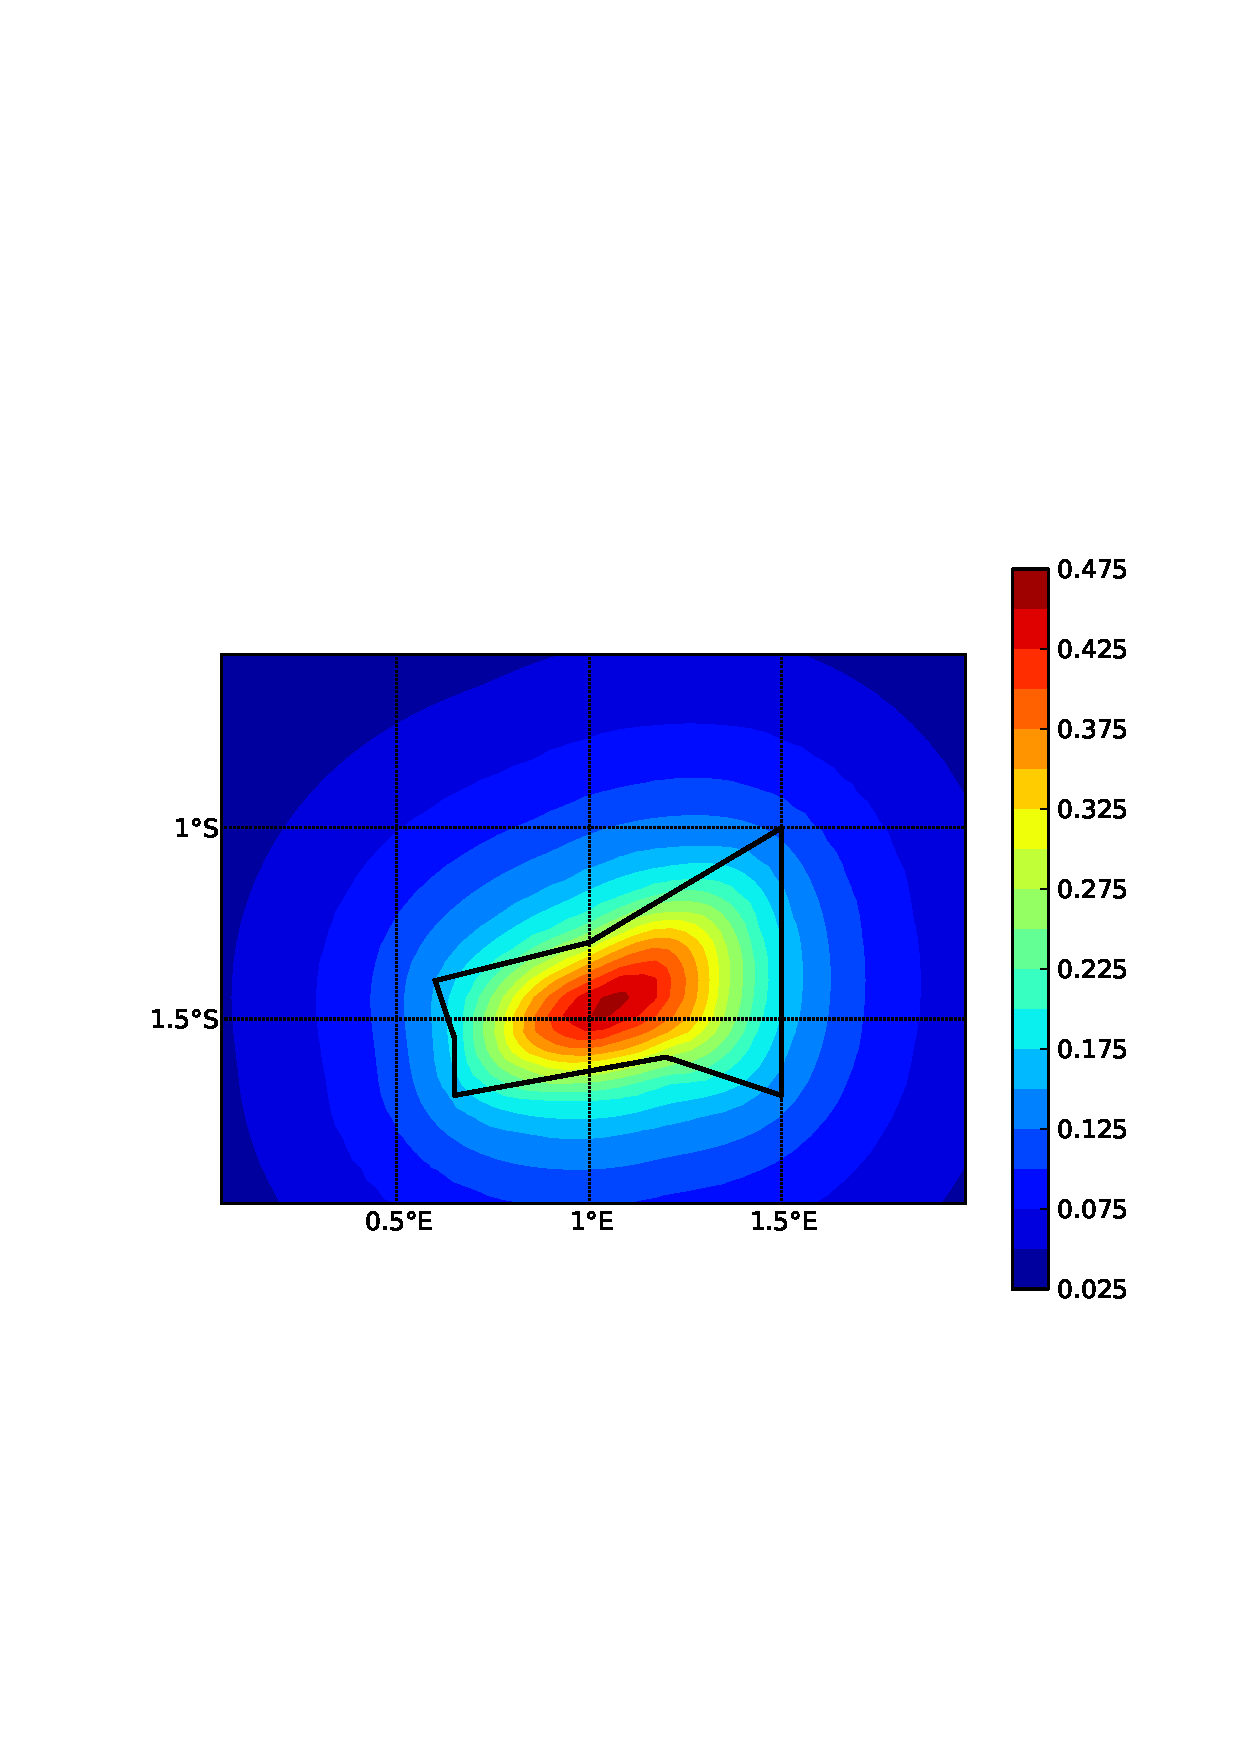
\includegraphics[width=7cm]{./figures/hazard/complex_fault.pdf}} 
\caption{Hazard maps (for PGA, 10\% in 50 years) as obtained from the different \gls{acr:oqe} source typologies. (a) Point Source. (b) Area source. 
The solid black line represents the area boundary. (c) Simple Fault Source. The dashed line represents the fault trace, while the solid line the fault
surface projection. (d) Complex Fault Source. The solid line represent the fault surface projection (d)}
\label{fig:hazard_maps1}
\end{figure}

\begin{figure} 
\centering 
\subcaptionbox{}
{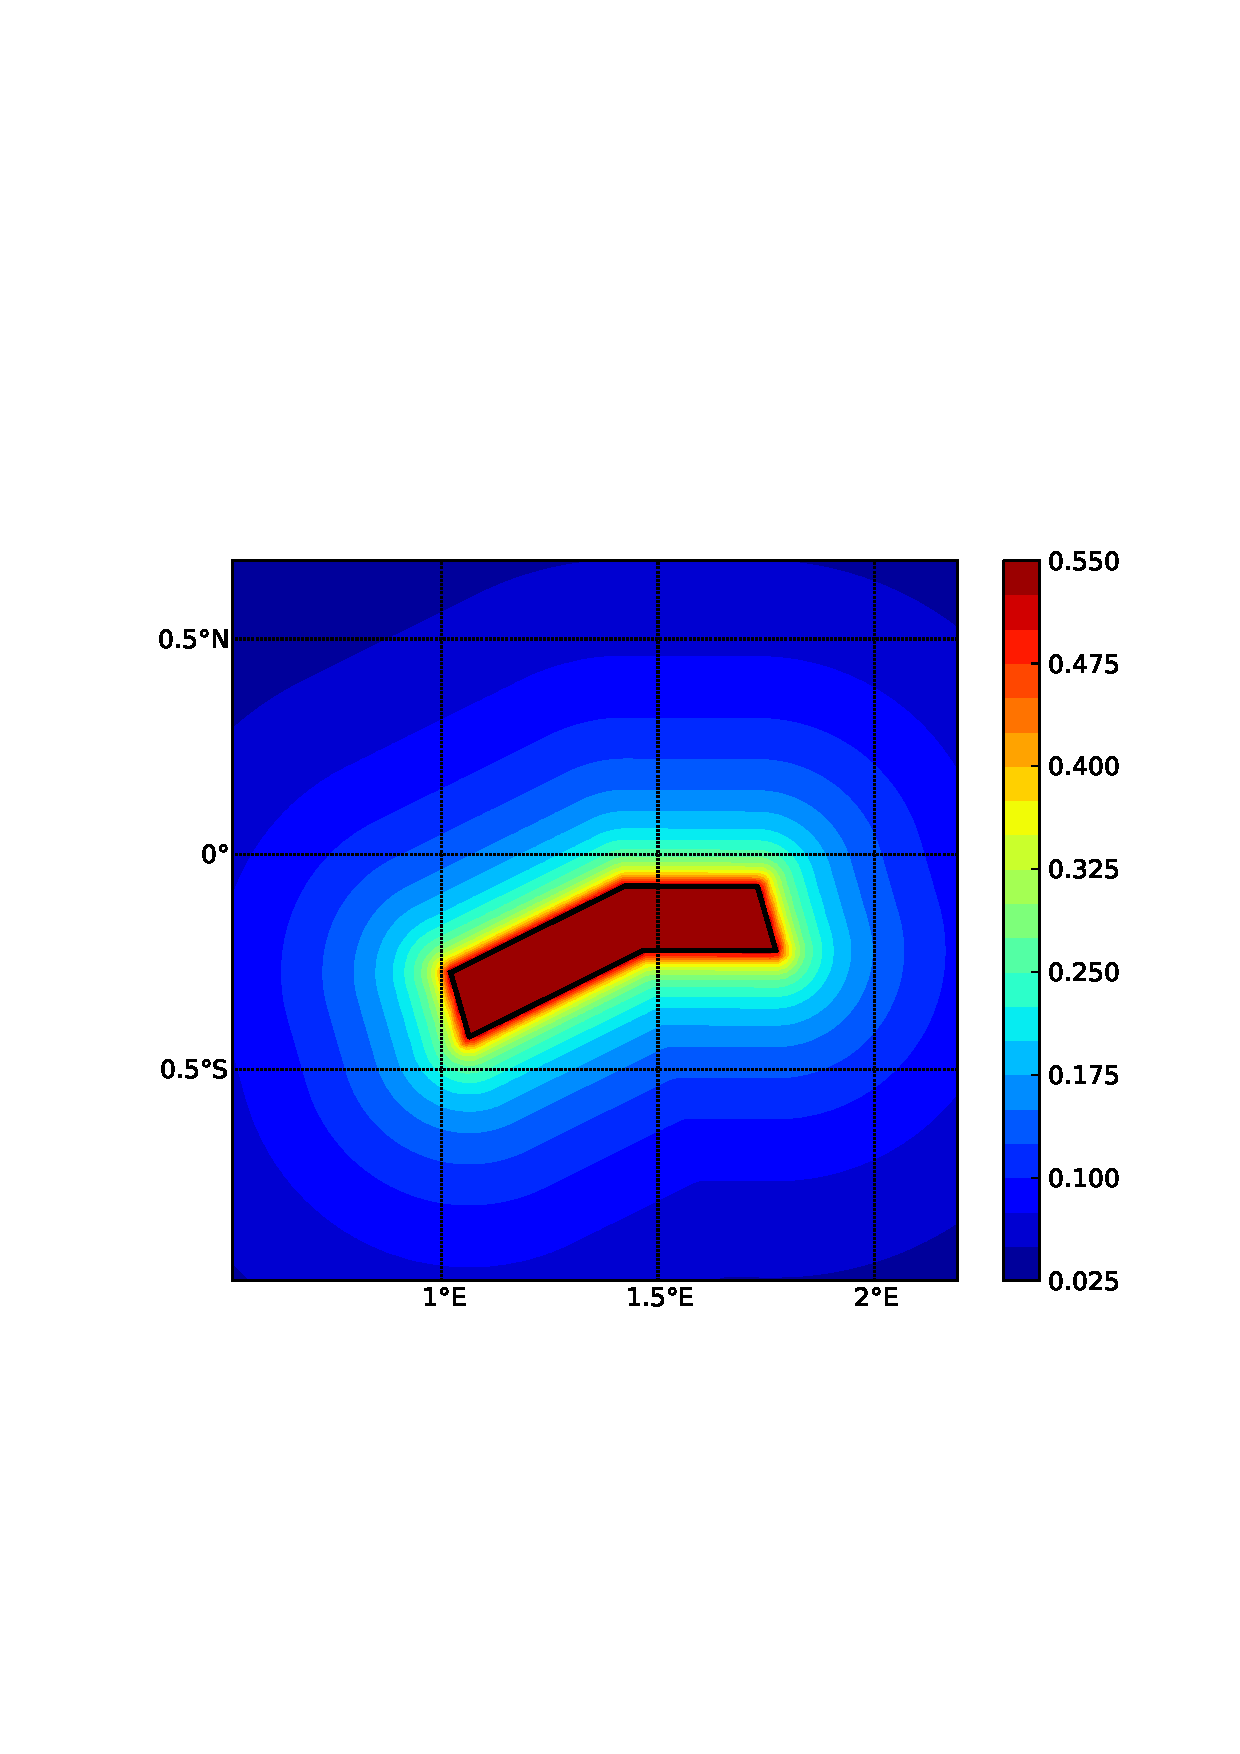
\includegraphics[width=7cm]{./figures/hazard/char_fault2.pdf}} 
\subcaptionbox{}
{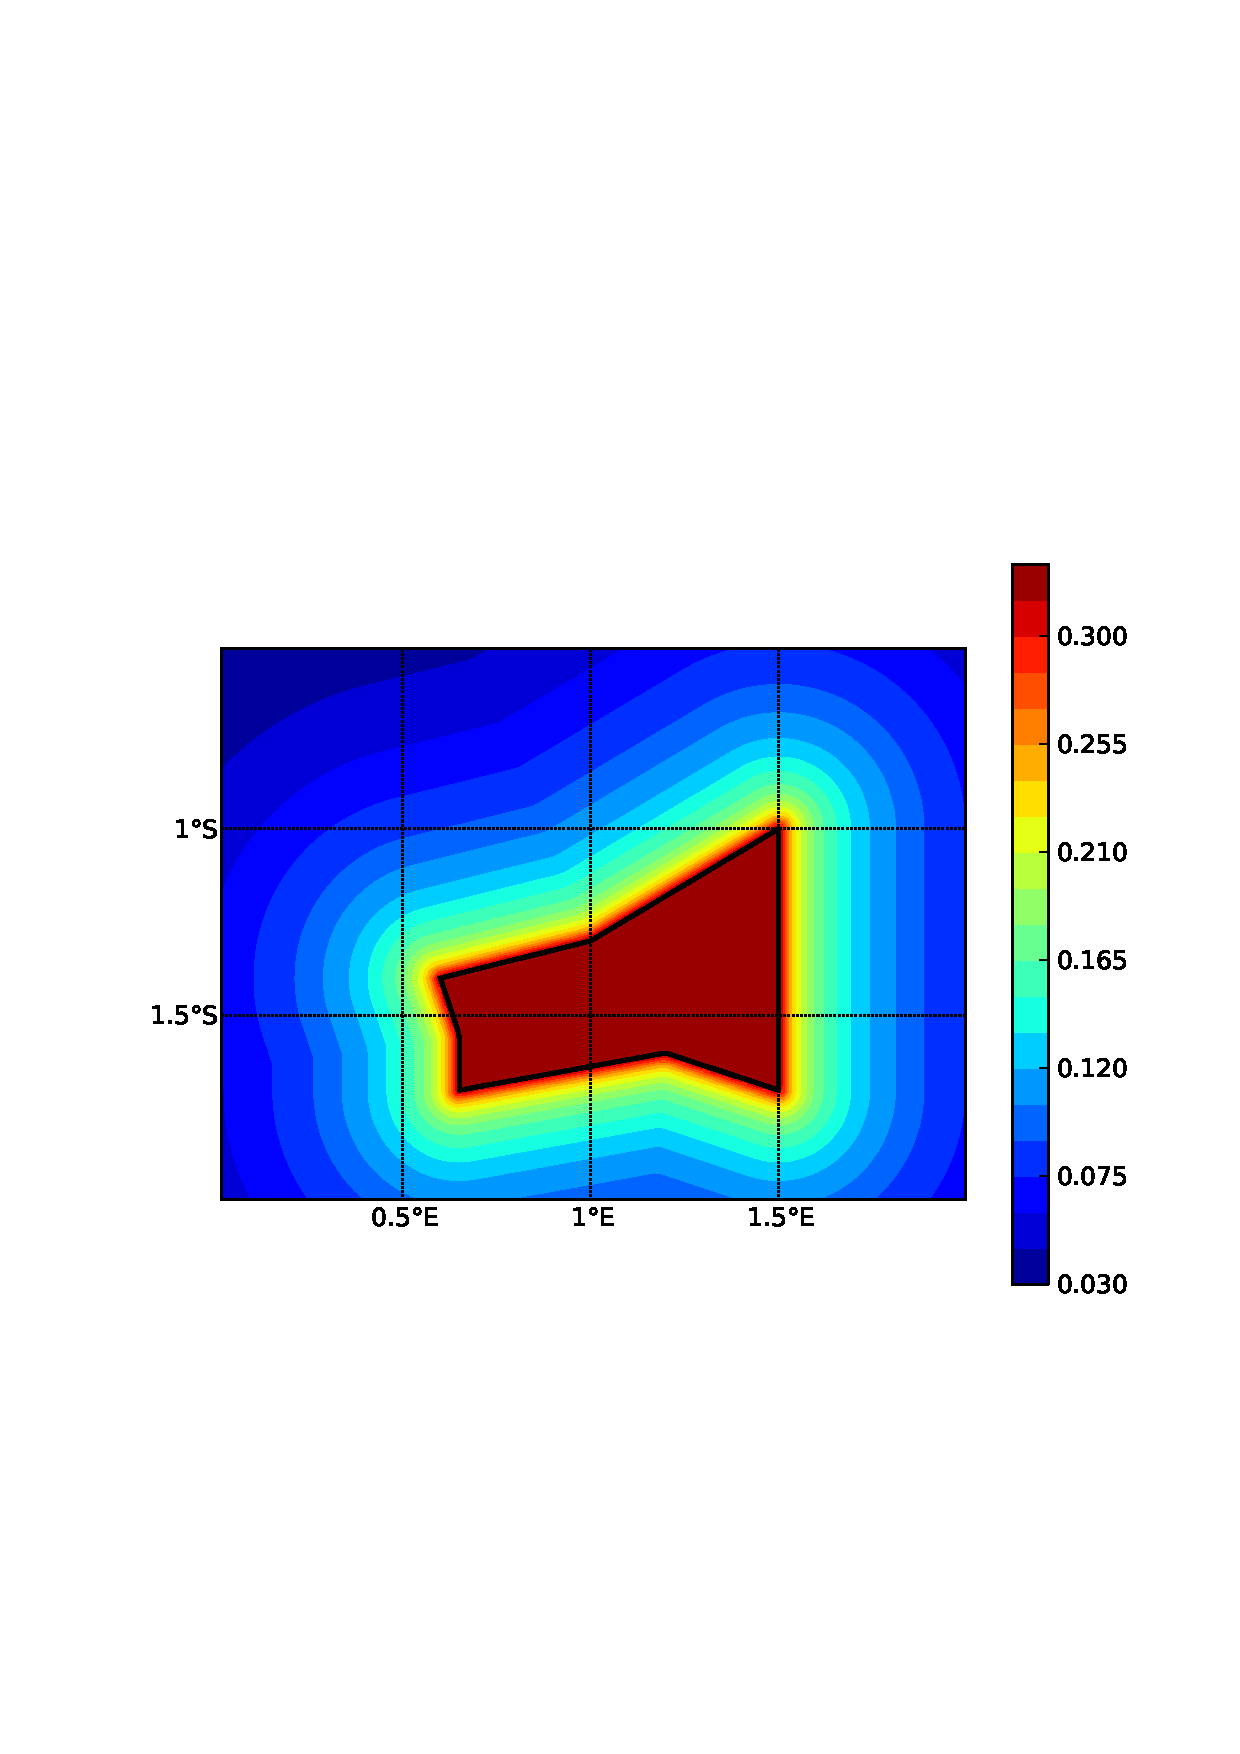
\includegraphics[width=7cm]{./figures/hazard/char_fault3.pdf}} 
\subcaptionbox{}
{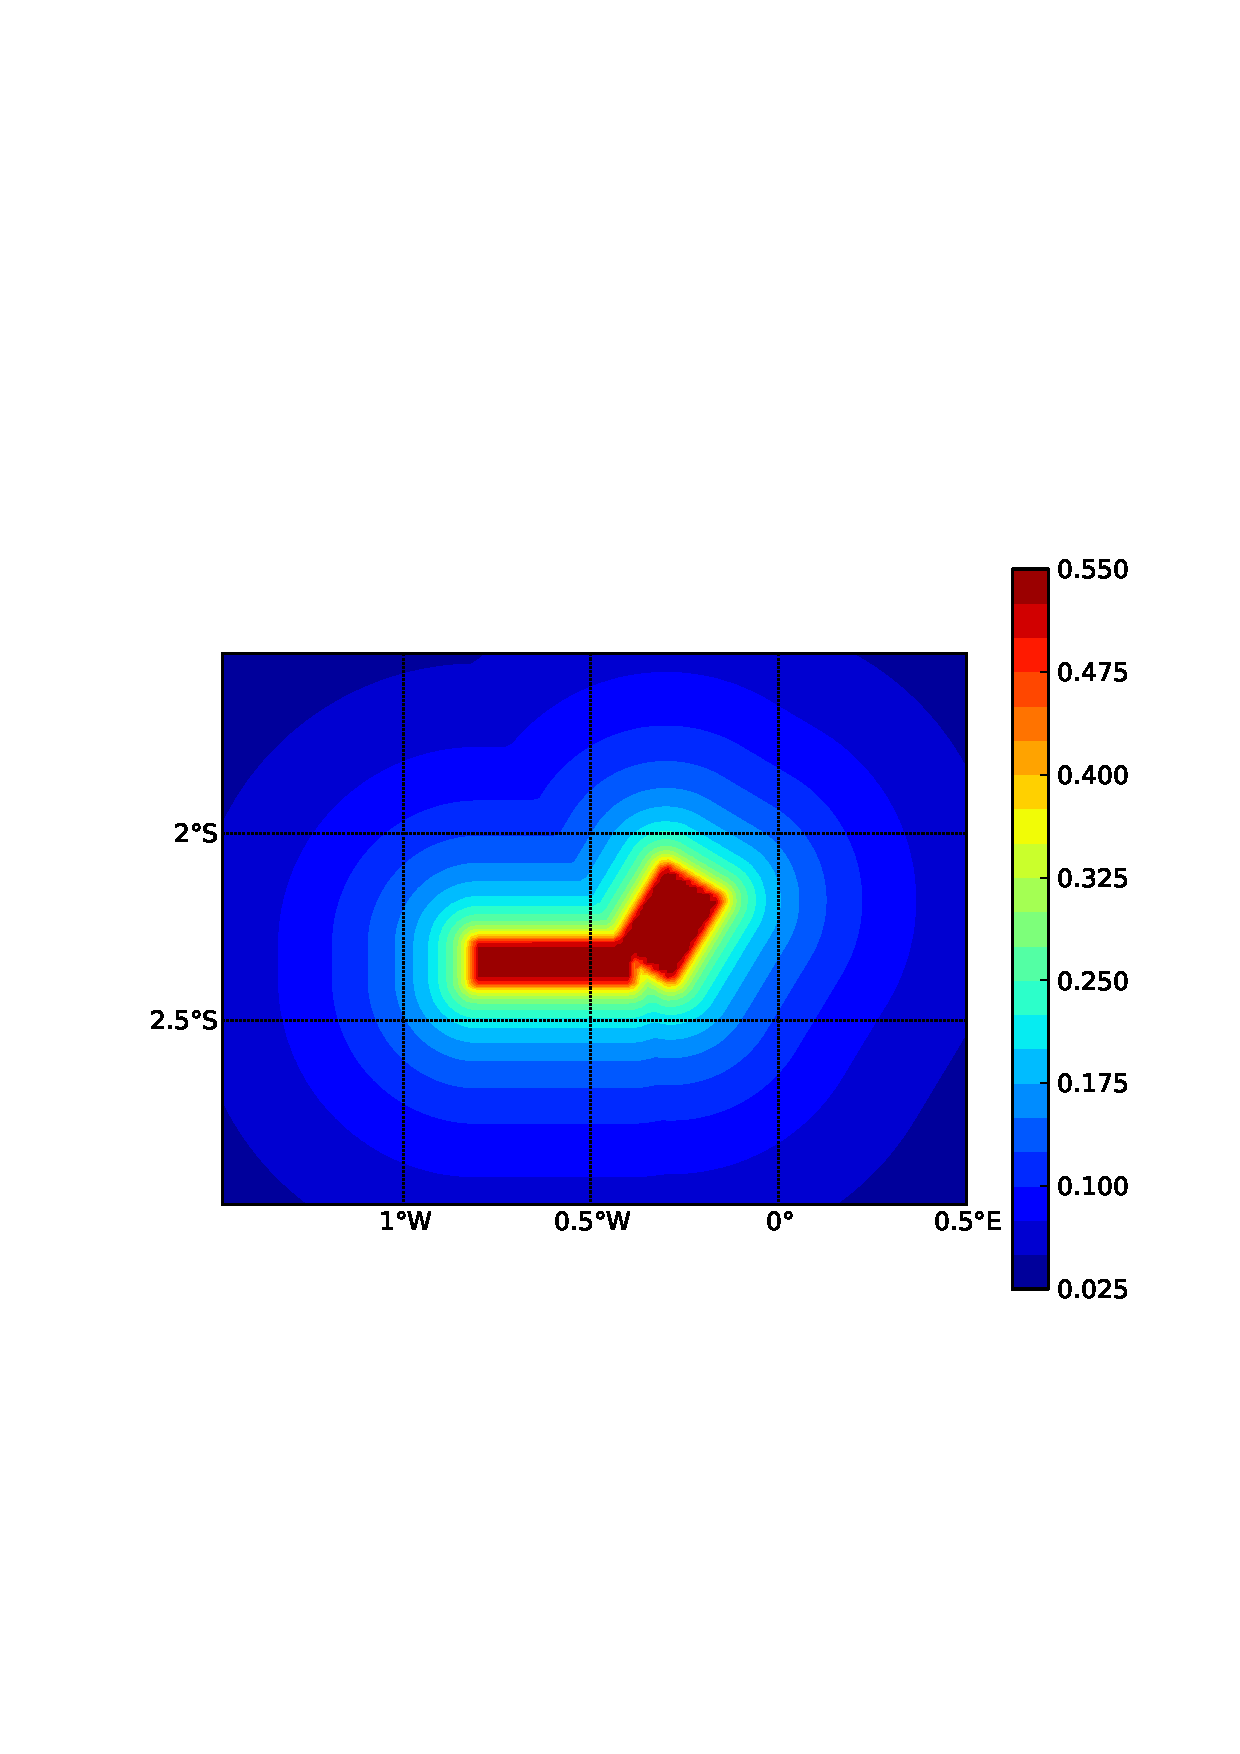
\includegraphics[width=7cm]{./figures/hazard/char_fault1.pdf}} 
\caption{Hazard maps (for PGA, 10\% in 50 years) as obtained from characteristic fault sources with simple fault
geometry (e), complex fault geometry (f), and collection of planar surfaces (g)}
\label{fig:hazard_maps2}
\end{figure}


\subsubsection{Classical PSHA with non trivial logic trees}
Three demos are provided to illustrate how the logic tree formalism can be used to express epistemic uncertainties in seismic hazard analysis.\\

LogicTreeCase1ClassicalPSHA shows an example of logic tree defining two alternative source models, with sources belonging to two different
tectonic region types, and with two alternative GMPEs for each tectonic region type.
The source model logic tree is therefore defined in the following way:
\begin{Verbatim}[frame=single, commandchars=\\\{\}, fontsize=\normalsize]
<?xml version="1.0" encoding="UTF-8"?>
<nrml xmlns:gml="http://www.opengis.net/gml"
      xmlns="http://openquake.org/xmlns/nrml/0.4">
    <logicTree logicTreeID="lt1">

        <logicTreeBranchingLevel branchingLevelID="bl1">

            <logicTreeBranchSet uncertaintyType="sourceModel"
                                branchSetID="bs1">
                <logicTreeBranch branchID="b1">
                    <uncertaintyModel>
                      source_model_1.xml
                    </uncertaintyModel>
                    <uncertaintyWeight>0.5</uncertaintyWeight>
                </logicTreeBranch>
                <logicTreeBranch branchID="b2">
                    <uncertaintyModel>
                       source_model_2.xml
                    </uncertaintyModel>
                    <uncertaintyWeight>0.5</uncertaintyWeight>
                </logicTreeBranch>
            </logicTreeBranchSet>

        </logicTreeBranchingLevel>

    </logicTree>
</nrml>
\end{Verbatim}
The two source models are defined in two different source model files \texttt{source\_\-model\_\-1.xml} and \texttt{source\_\-model\_\-2.xml} each
associated to the corresponding weight (0.5 in both cases).\\
The GSIM logic tree file contains the following structure:
\begin{Verbatim}[frame=single, commandchars=\\\{\}, fontsize=\normalsize]
<?xml version="1.0" encoding="UTF-8"?>

<nrml xmlns:gml="http://www.opengis.net/gml"
      xmlns="http://openquake.org/xmlns/nrml/0.4">
    <logicTree logicTreeID='lt1'>

        <logicTreeBranchingLevel branchingLevelID="bl1">
            <logicTreeBranchSet uncertaintyType="gmpeModel"
               applyToTectonicRegionType="Active Shallow Crust"
               branchSetID="bs1">
                <logicTreeBranch branchID="b11">
                   <uncertaintyModel>
                      BooreAtkinson2008
                   </uncertaintyModel>
                   <uncertaintyWeight>0.5</uncertaintyWeight>
                </logicTreeBranch>
                <logicTreeBranch branchID="b12">
                   <uncertaintyModel>
                      ChiouYoungs2008
                   </uncertaintyModel>
                   <uncertaintyWeight>0.5</uncertaintyWeight>
                </logicTreeBranch>
            </logicTreeBranchSet>
        </logicTreeBranchingLevel>

        <logicTreeBranchingLevel branchingLevelID="bl2">
            <logicTreeBranchSet uncertaintyType="gmpeModel"
              applyToTectonicRegionType="Stable Continental Crust"
              branchSetID="bs2">
              <logicTreeBranch branchID="b21">
                <uncertaintyModel>
                   ToroEtAl2002</uncertaintyModel>
                <uncertaintyWeight>0.5</uncertaintyWeight>
                </logicTreeBranch>
                <logicTreeBranch branchID="b22">
                  <uncertaintyModel>
                     Campbell2003</uncertaintyModel>
                  <uncertaintyWeight>0.5</uncertaintyWeight>
                </logicTreeBranch>
            </logicTreeBranchSet>
        </logicTreeBranchingLevel>

    </logicTree>
</nrml>
\end{Verbatim}
The source model contains sources belonging to Active Shallow Crust and Stable Continental Crust, therefore the
GSIM logic tree defines two branching levels, one for each considered tectonic region type. Moreover for each tectonic
region type a branch set with two GMPEs is defined: Boore and Atkinson 2008 and Chiou and Youngs 2008 for Active
Shallow Crust and Toro et al. 2003 and Campbell 2003 for Stable Continental Crust. By processing the above logic tree
files using the logic tree path enumeration mode (enabled by setting in the configuration file \texttt{number\_\-of\_\-logic\_\-tree\_\-samples = 0})
hazard results are obtained for 8 logic tree paths (2 source models x 2 GMPEs for Active x 2 GMPEs for Stable).\\

LogicTreeCase2ClassicalPSHA defines a single source model consisting of only two sources (area and simple fault) belonging to different
tectonic region types (Active Shallow Crust and Stable Continental Region) and both characterized by a truncated Gutenberg-Richter distribution.
The logic tree defines uncertainties for G-R a, b values (three possible pairs for each source) and maximum magnitude (three values for each source) 
and uncertainties on the GMPEs for each tectonic region type (two GMPE per region type).\\
To accomodate such a structure the GSIM logic tree is defined in the following way:
\begin{Verbatim}[frame=single, commandchars=\\\{\}, fontsize=\normalsize]
<?xml version="1.0" encoding="UTF-8"?>
<nrml xmlns:gml="http://www.opengis.net/gml"
      xmlns="http://openquake.org/xmlns/nrml/0.4">
    <logicTree logicTreeID="lt1">

        <logicTreeBranchingLevel branchingLevelID="bl1">
            <logicTreeBranchSet uncertaintyType="sourceModel"
                                branchSetID="bs1">
                <logicTreeBranch branchID="b11">
                    <uncertaintyModel>
                     source_model.xml
                    </uncertaintyModel>
                    <uncertaintyWeight>1.0</uncertaintyWeight>
                </logicTreeBranch>
            </logicTreeBranchSet>
        </logicTreeBranchingLevel>

        <logicTreeBranchingLevel branchingLevelID="bl2">
            <logicTreeBranchSet uncertaintyType="abGRAbsolute"
                                applyToSources="1"
                                branchSetID="bs21">
                <logicTreeBranch branchID="b21">
                    <uncertaintyModel>4.6 1.1</uncertaintyModel>
                    <uncertaintyWeight>0.333</uncertaintyWeight>
                </logicTreeBranch>
                <logicTreeBranch branchID="b22">
                    <uncertaintyModel>4.5 1.0</uncertaintyModel>
                    <uncertaintyWeight>0.333</uncertaintyWeight>
                </logicTreeBranch>
                <logicTreeBranch branchID="b23">
                    <uncertaintyModel>4.4 0.9</uncertaintyModel>
                    <uncertaintyWeight>0.334</uncertaintyWeight>
                </logicTreeBranch>
            </logicTreeBranchSet>
        </logicTreeBranchingLevel>

        <logicTreeBranchingLevel branchingLevelID="bl3">
            <logicTreeBranchSet uncertaintyType="abGRAbsolute"
                                applyToSources="2"
                                branchSetID="bs31">
                <logicTreeBranch branchID="b31">
                    <uncertaintyModel>3.3 1.0</uncertaintyModel>
                    <uncertaintyWeight>0.333</uncertaintyWeight>
                </logicTreeBranch>
                <logicTreeBranch branchID="b32">
                    <uncertaintyModel>3.2 0.9</uncertaintyModel>
                    <uncertaintyWeight>0.333</uncertaintyWeight>
                </logicTreeBranch>
                <logicTreeBranch branchID="b33">
                    <uncertaintyModel>3.1 0.8</uncertaintyModel>
                    <uncertaintyWeight>0.334</uncertaintyWeight>
                </logicTreeBranch>
            </logicTreeBranchSet>
        </logicTreeBranchingLevel>

        <logicTreeBranchingLevel branchingLevelID="bl4">
            <logicTreeBranchSet uncertaintyType="maxMagGRAbsolute"
                                applyToSources="1"
                                branchSetID="bs41">
                <logicTreeBranch branchID="b41">
                    <uncertaintyModel>7.0</uncertaintyModel>
                    <uncertaintyWeight>0.333</uncertaintyWeight>
                </logicTreeBranch>
                <logicTreeBranch branchID="b42">
                    <uncertaintyModel>7.3</uncertaintyModel>
                    <uncertaintyWeight>0.333</uncertaintyWeight>
                </logicTreeBranch>
                <logicTreeBranch branchID="b43">
                    <uncertaintyModel>7.6</uncertaintyModel>
                    <uncertaintyWeight>0.334</uncertaintyWeight>
                </logicTreeBranch>
            </logicTreeBranchSet>
        </logicTreeBranchingLevel>

        <logicTreeBranchingLevel branchingLevelID="bl5">
            <logicTreeBranchSet uncertaintyType="maxMagGRAbsolute"
                                applyToSources="2"
                                branchSetID="bs51">
                <logicTreeBranch branchID="b51">
                    <uncertaintyModel>7.5</uncertaintyModel>
                    <uncertaintyWeight>0.333</uncertaintyWeight>
                </logicTreeBranch>
                <logicTreeBranch branchID="b52">
                    <uncertaintyModel>7.8</uncertaintyModel>
                    <uncertaintyWeight>0.333</uncertaintyWeight>
                </logicTreeBranch>
                <logicTreeBranch branchID="b53">
                    <uncertaintyModel>8.0</uncertaintyModel>
                    <uncertaintyWeight>0.334</uncertaintyWeight>
                </logicTreeBranch>
            </logicTreeBranchSet>
        </logicTreeBranchingLevel>

    </logicTree>
</nrml>
\end{Verbatim}
The first branching level defines the source model. For each source, two branching levels are created, one defining
uncertainties on G-R a and b values (defined by setting \texttt{uncertaintyType="abGRAbsolute"}) and G-R maximum
magnitude (\texttt{uncertaintyType="maxMagGRAbsolute"}). It is important to notice that each branch set is applied
to a specific source by defining the attribute \texttt{applyToSources}, followed by the source ID. The GSIM logic tree file is
the same as used for LogicTreeCas1ClassicalPSHA. By setting in the configuration file \texttt{number\_\-of\_\-logic\_\-tree\_\-samples = 0},
hazard results are obtained for 324 paths (1 source model x 3 (a, b) pairs for source 1 x  3 (a, b) pairs for source 2 x 3 max magnitude values
for source 1 x 3 max magnitude values for source 2 x 2 GMPEs for Active Shallow Crust X 2 GMPEs for Stable Continental Crust), see
figure \ref{fig:hazard_curves}.\\

\begin{figure}
\centering
\subcaptionbox{}
{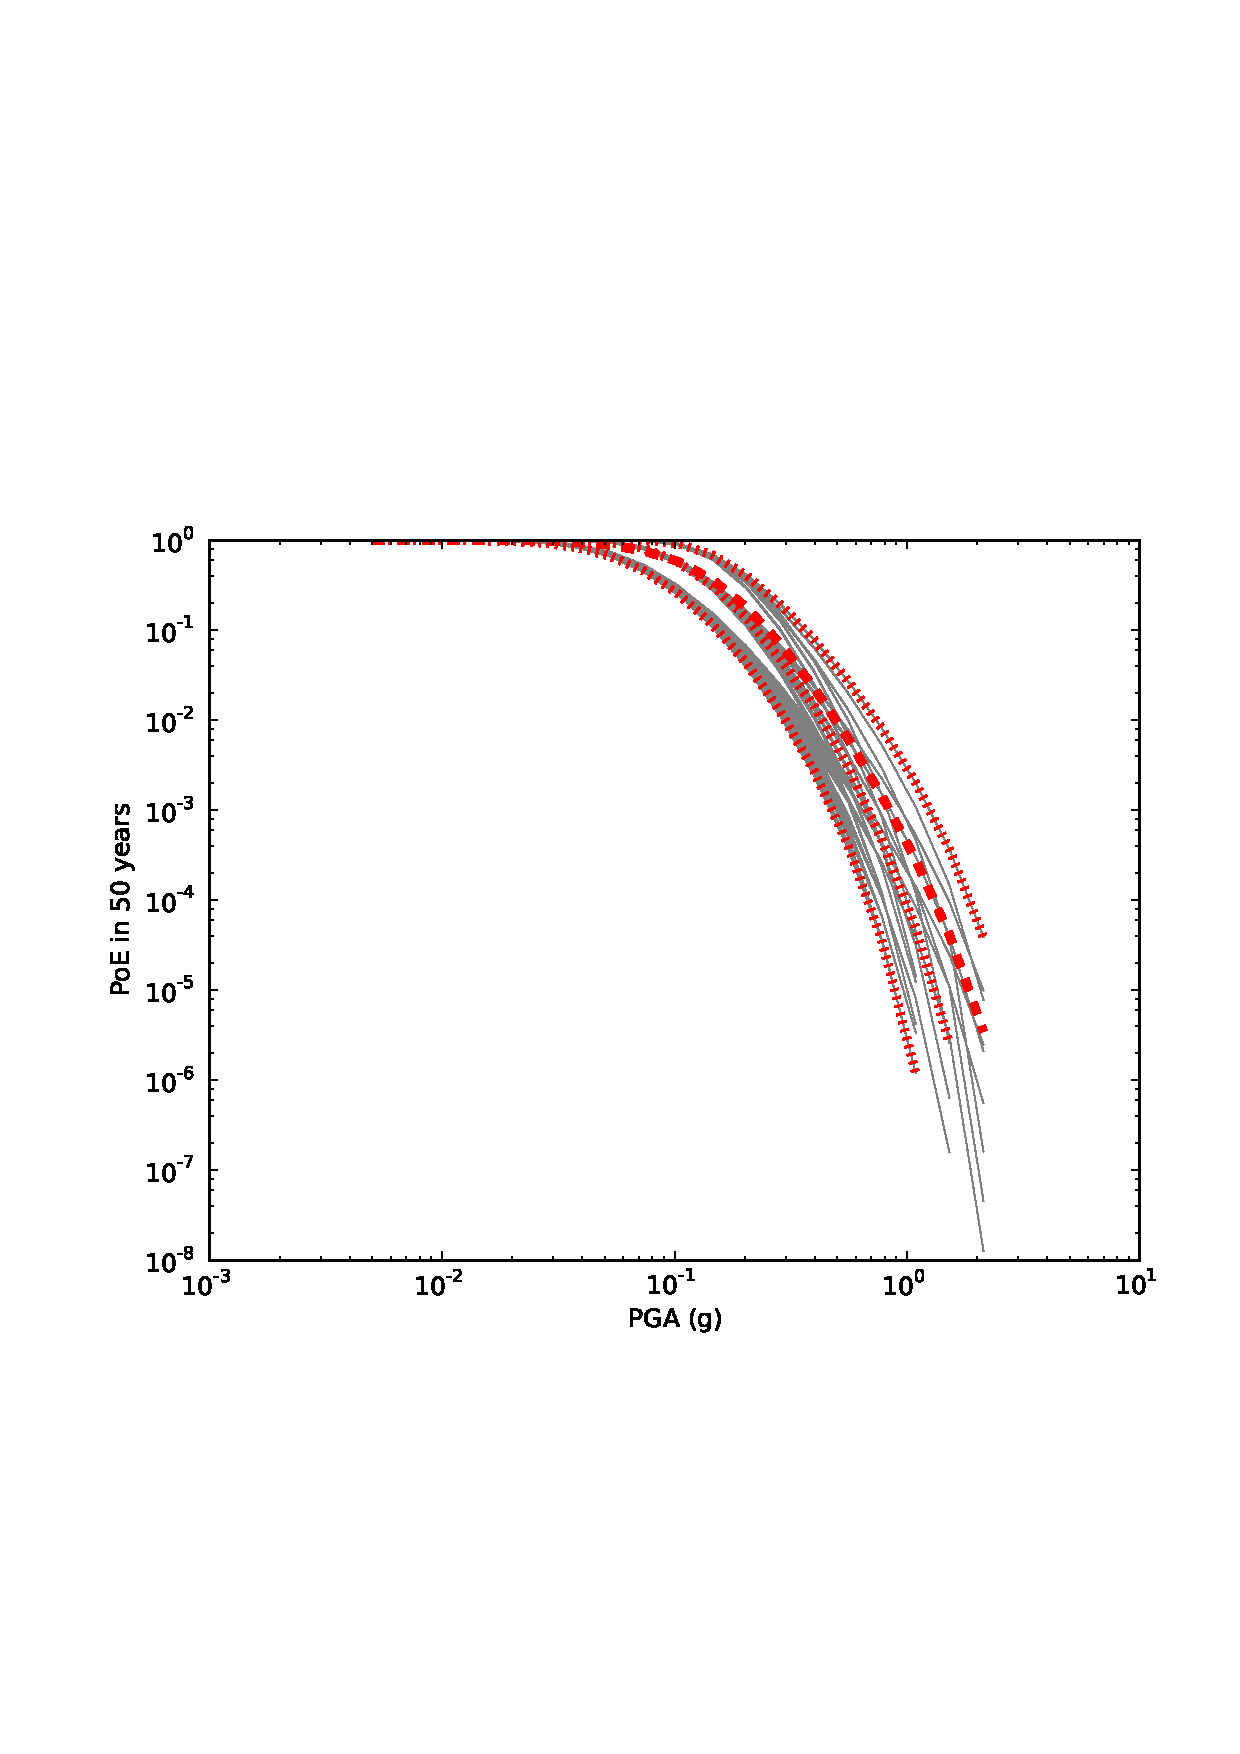
\includegraphics[width=9cm]{./figures/hazard/hazard-curves-ltcase2.pdf}}
\caption{Hazard curves as obtained from the LogicTreeCase2 demo. Solid gray lines represent individual hazard curves from the different
logic tree path (a total of 324 curves). The red dashed line represents the mean hazard curve, while the red dotted lines depict the quantile levels
(0.15, 0.5, 0.95).}
\label{fig:hazard_curves}
\end{figure}

LogicTreeCase3ClassicalPSHA illustrates an example of logic tree defining relative uncertainties on G-R maximum magnitude and b value.
A single source model is considered containing two sources belonging to different tectonic region types and both characterized by a G-R 
magnitude frequency distribution. The source model logic tree is as follows:
\begin{Verbatim}[frame=single, commandchars=\\\{\}, fontsize=\normalsize]
<?xml version="1.0" encoding="UTF-8"?>
<nrml xmlns:gml="http://www.opengis.net/gml"
      xmlns="http://openquake.org/xmlns/nrml/0.4">
    <logicTree logicTreeID="lt1">

        <logicTreeBranchingLevel branchingLevelID="bl1">
            <logicTreeBranchSet uncertaintyType="sourceModel"
                                branchSetID="bs1">
                <logicTreeBranch branchID="b11">
                    <uncertaintyModel>
                     source_model.xml
                    </uncertaintyModel>
                    <uncertaintyWeight>1.0</uncertaintyWeight>
                </logicTreeBranch>
            </logicTreeBranchSet>
        </logicTreeBranchingLevel>

        <logicTreeBranchingLevel branchingLevelID="bl2">
            <logicTreeBranchSet uncertaintyType="bGRRelative"
                                branchSetID="bs21">
                <logicTreeBranch branchID="b21">
                    <uncertaintyModel>+0.1</uncertaintyModel>
                    <uncertaintyWeight>0.333</uncertaintyWeight>
                </logicTreeBranch>
                <logicTreeBranch branchID="b22">
                    <uncertaintyModel>0.0</uncertaintyModel>
                    <uncertaintyWeight>0.333</uncertaintyWeight>
                </logicTreeBranch>
                <logicTreeBranch branchID="b23">
                    <uncertaintyModel>-0.1</uncertaintyModel>
                    <uncertaintyWeight>0.334</uncertaintyWeight>
                </logicTreeBranch>
            </logicTreeBranchSet>
        </logicTreeBranchingLevel>

        <logicTreeBranchingLevel branchingLevelID="bl3">
            <logicTreeBranchSet uncertaintyType="maxMagGRRelative"
                                branchSetID="bs31">
                <logicTreeBranch branchID="b31">
                    <uncertaintyModel>0.0</uncertaintyModel>
                    <uncertaintyWeight>0.333</uncertaintyWeight>
                </logicTreeBranch>
                <logicTreeBranch branchID="b32">
                    <uncertaintyModel>+0.5</uncertaintyModel>
                    <uncertaintyWeight>0.333</uncertaintyWeight>
                </logicTreeBranch>
                <logicTreeBranch branchID="b33">
                    <uncertaintyModel>+1.0</uncertaintyModel>
                    <uncertaintyWeight>0.334</uncertaintyWeight>
                </logicTreeBranch>
            </logicTreeBranchSet>
        </logicTreeBranchingLevel>

    </logicTree>
</nrml>
\end{Verbatim}
After the first branching level defining the source model, two additional branching levels are defined, one defining
relative uncertainties on b value (\texttt{bGRRelative} applied consistently to all sources in the source model)
and the second uncertainties on maximum magnitude (\texttt{maxMagGRRelative}). Similarly to the other cases,
two GMPEs are considered for each tectonic region type and therefore the total number of logic tree path is 36
(1 source model x 3 b value increments x 3 maximum magnitude increments x 2 GMPE for Active x 2 GMPEs for Stable)

\subsubsection{Event Based PSHA}
A demo showing an example of Event Based calculation is provided with the following configuration file:
\begin{Verbatim}[frame=single, commandchars=\\\{\}, fontsize=\normalsize]
[general]

description = Event Based PSHA using Area Source
calculation_mode = event_based
random_seed = 23

[geometry]

sites = 0.5 -0.5

[logic_tree]

number_of_logic_tree_samples = 0

[erf]

rupture_mesh_spacing = 2
width_of_mfd_bin = 0.1
area_source_discretization = 5.0

[site_params]

reference_vs30_type = measured
reference_vs30_value = 600.0
reference_depth_to_2pt5km_per_sec = 5.0
reference_depth_to_1pt0km_per_sec = 100.0

[calculation]

source_model_logic_tree_file = source_model_logic_tree.xml
gsim_logic_tree_file = gmpe_logic_tree.xml
investigation_time = 50.0
intensity_measure_types_and_levels = {"PGA": [...]}
truncation_level = 3
maximum_distance = 200.0

[event_based_params]

ses_per_logic_tree_path = 100
ground_motion_correlation_model =
ground_motion_correlation_params =

[output]

export_dir = ...
ground_motion_fields = true
hazard_curves_from_gmfs = true
mean_hazard_curves = false
quantile_hazard_curves =
hazard_maps = true
poes = 0.1
\end{Verbatim}
The source model consist of one source (area). 100 stochastic event sets are generated (\texttt{ses\_\-per\_\-logic\_\-tree\_\-path = 100}) (an example can be seen
in figure \ref{fig:ses}). Ground motion fields are computed (\texttt{ground\_\-motion\_\-fields = true}, figure \ref{fig:gmfs}) and also hazard curves from ground motion fields are
extracted (\texttt{hazard\_\-curves\_\-from\_\-gmfs = true}).
Corresponding hazard maps for 0.1 probability are additionally calculated (\texttt{hazard\_\-maps = true})

\begin{figure} 
\centering 
\subcaptionbox{}
{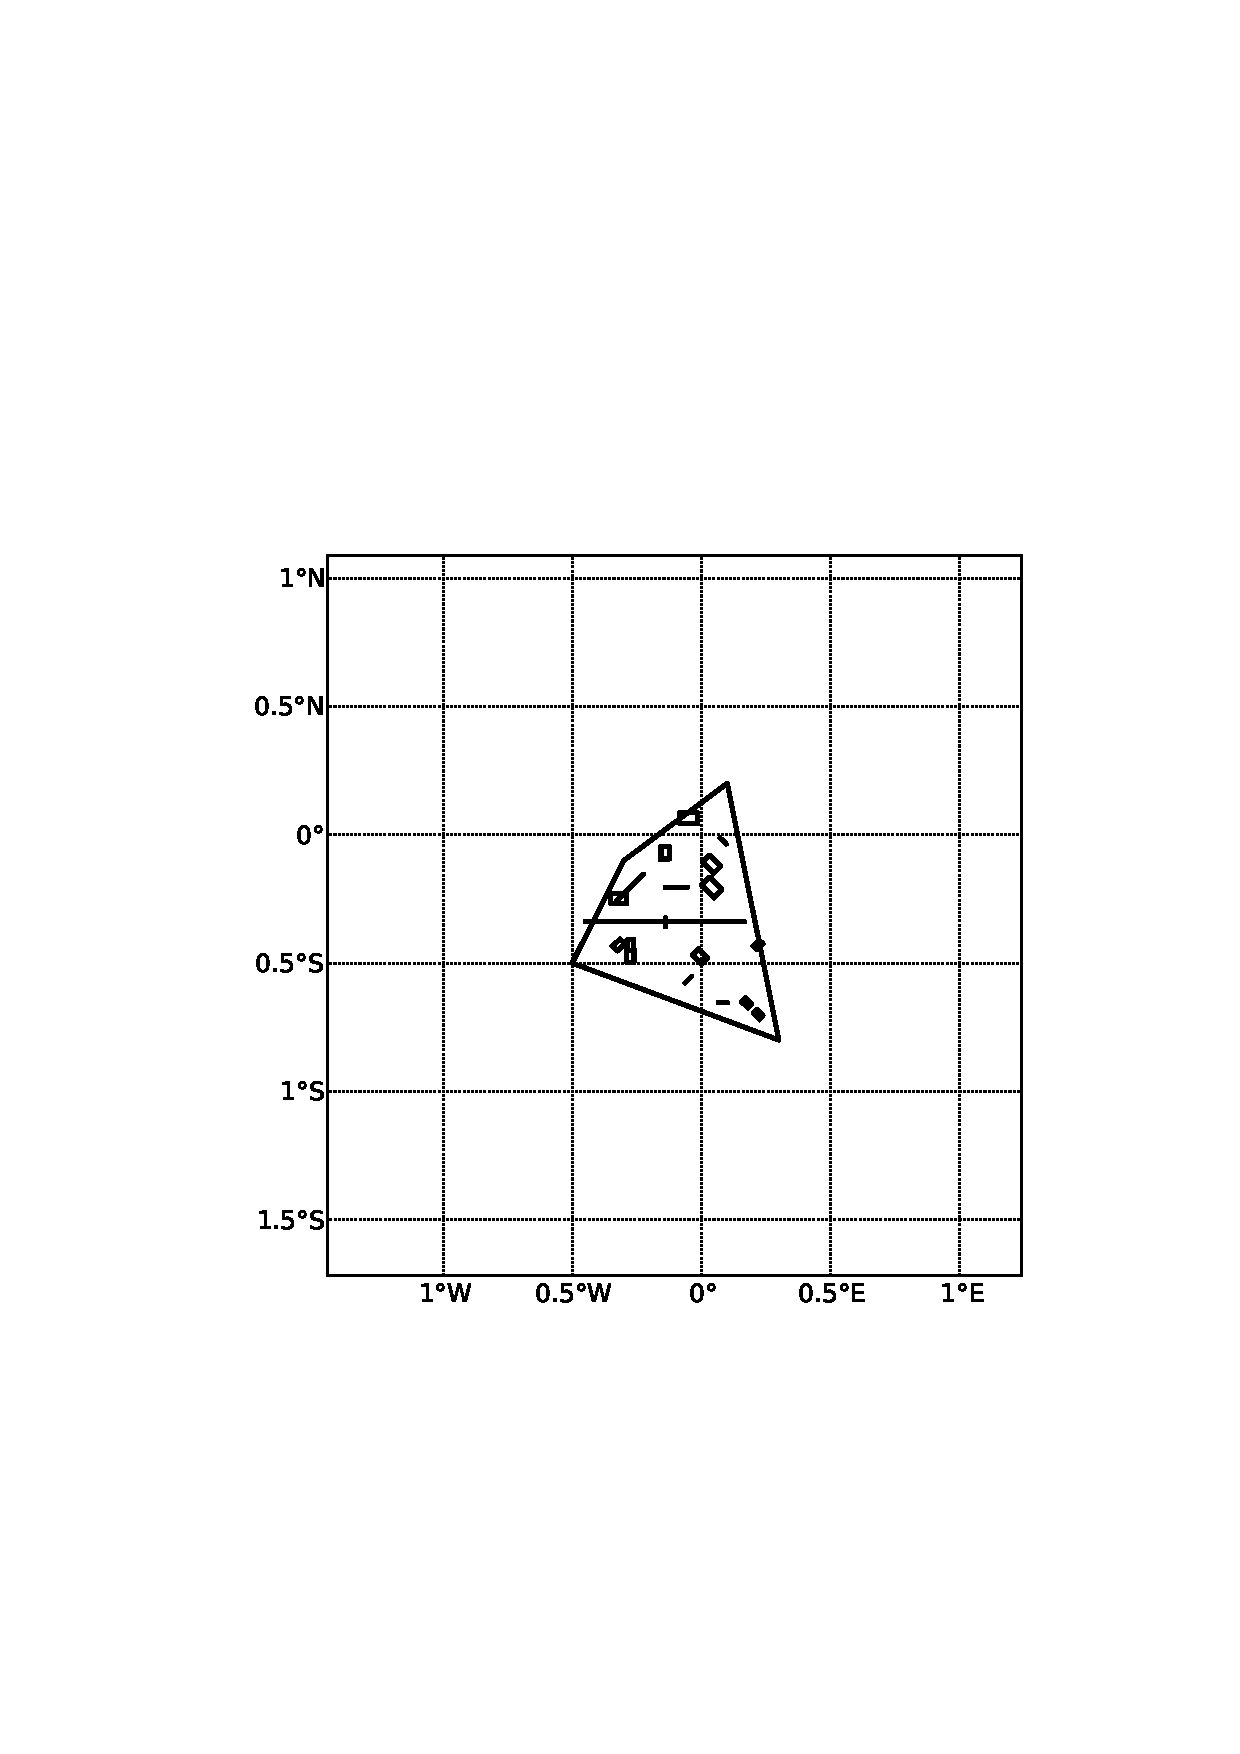
\includegraphics[width=9cm]{./figures/hazard/ses.pdf}} 
\caption{A stochastic event set generated in the event based PSHA demo. The area source defines a nodal plane distribution which distributes events among vertical and
dipping (50 degrees) faults with equal weights. Vertical ruptures are then distributed equally in the range 0-180 degrees while the dipping ones in the range 0-360, both
with a step of 45 degrees.}
\label{fig:ses}
\end{figure}

\begin{figure} 
\centering 
\subcaptionbox{}
{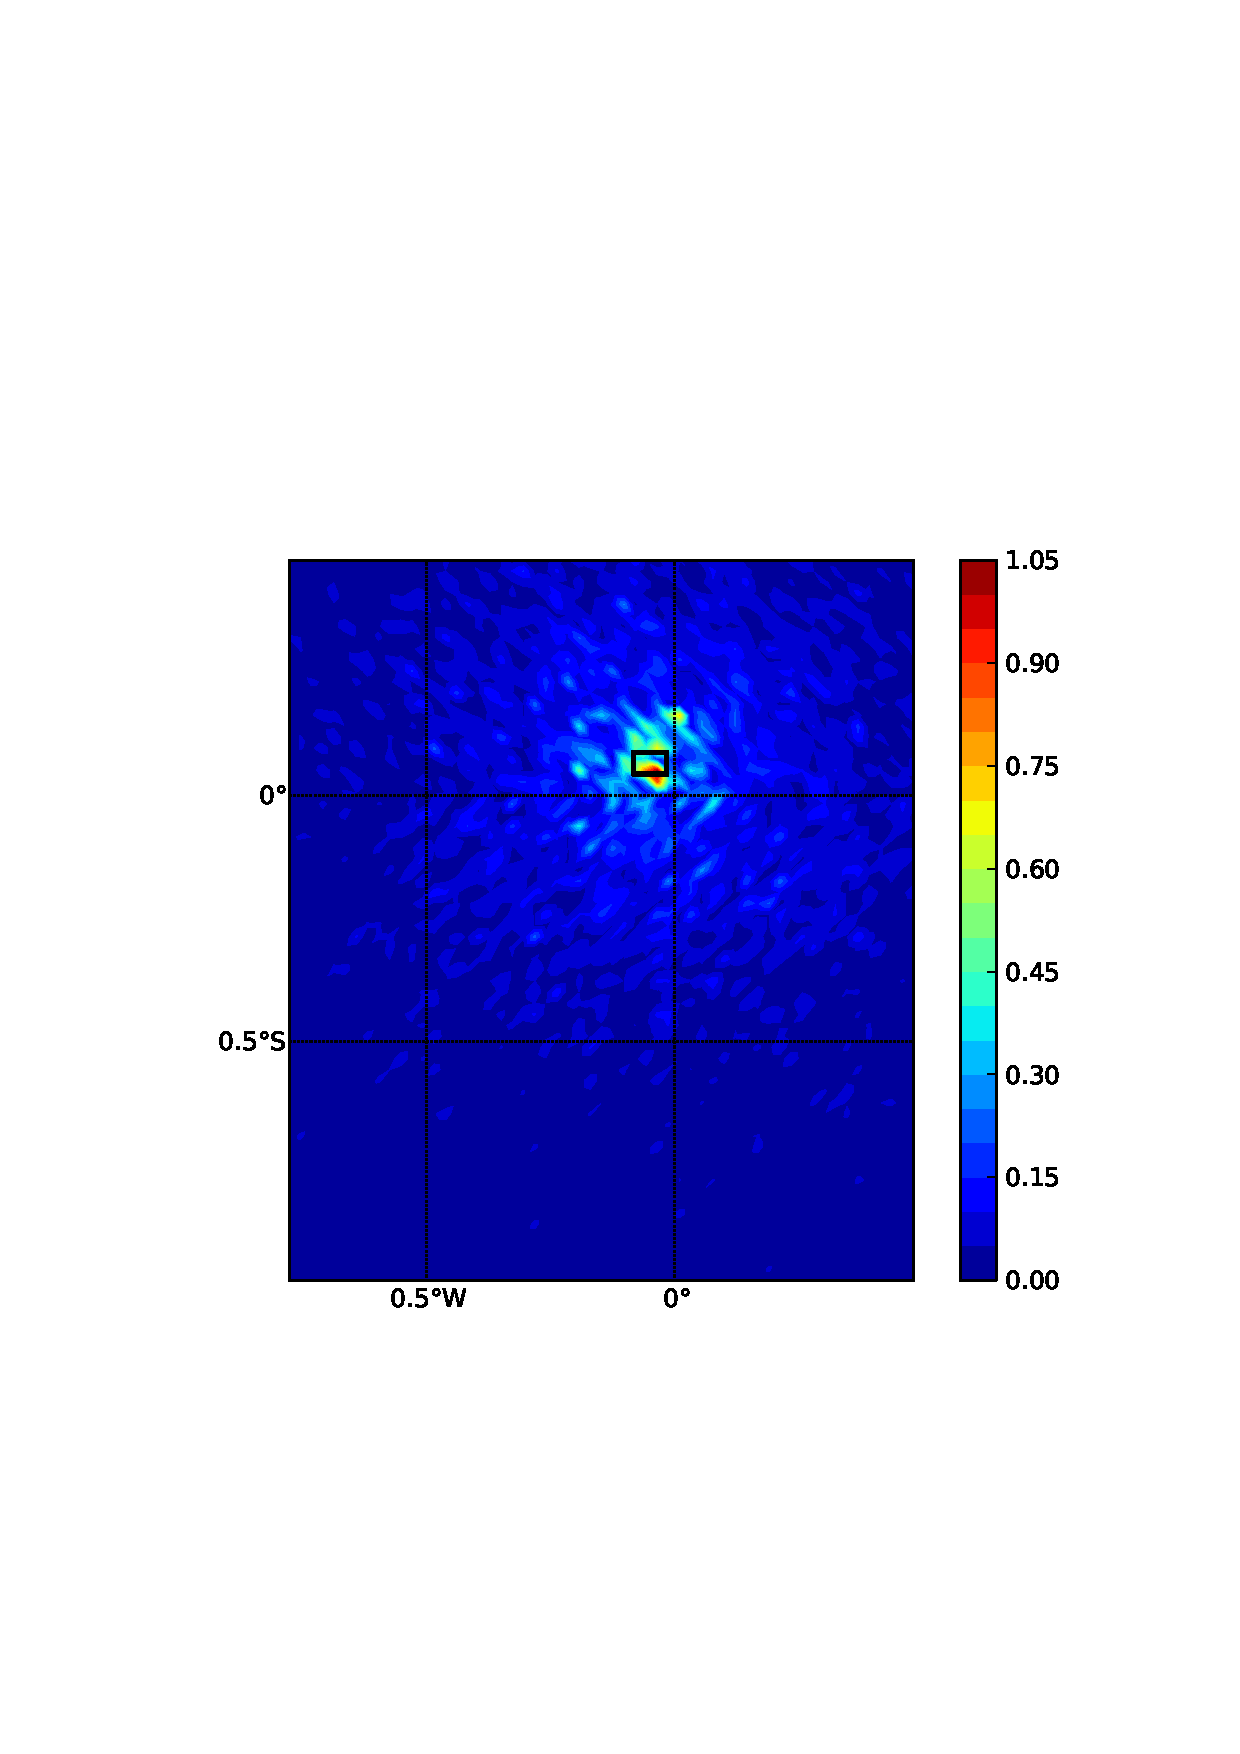
\includegraphics[width=6cm]{./figures/hazard/gmf-no-corr.pdf}} 
\subcaptionbox{}
{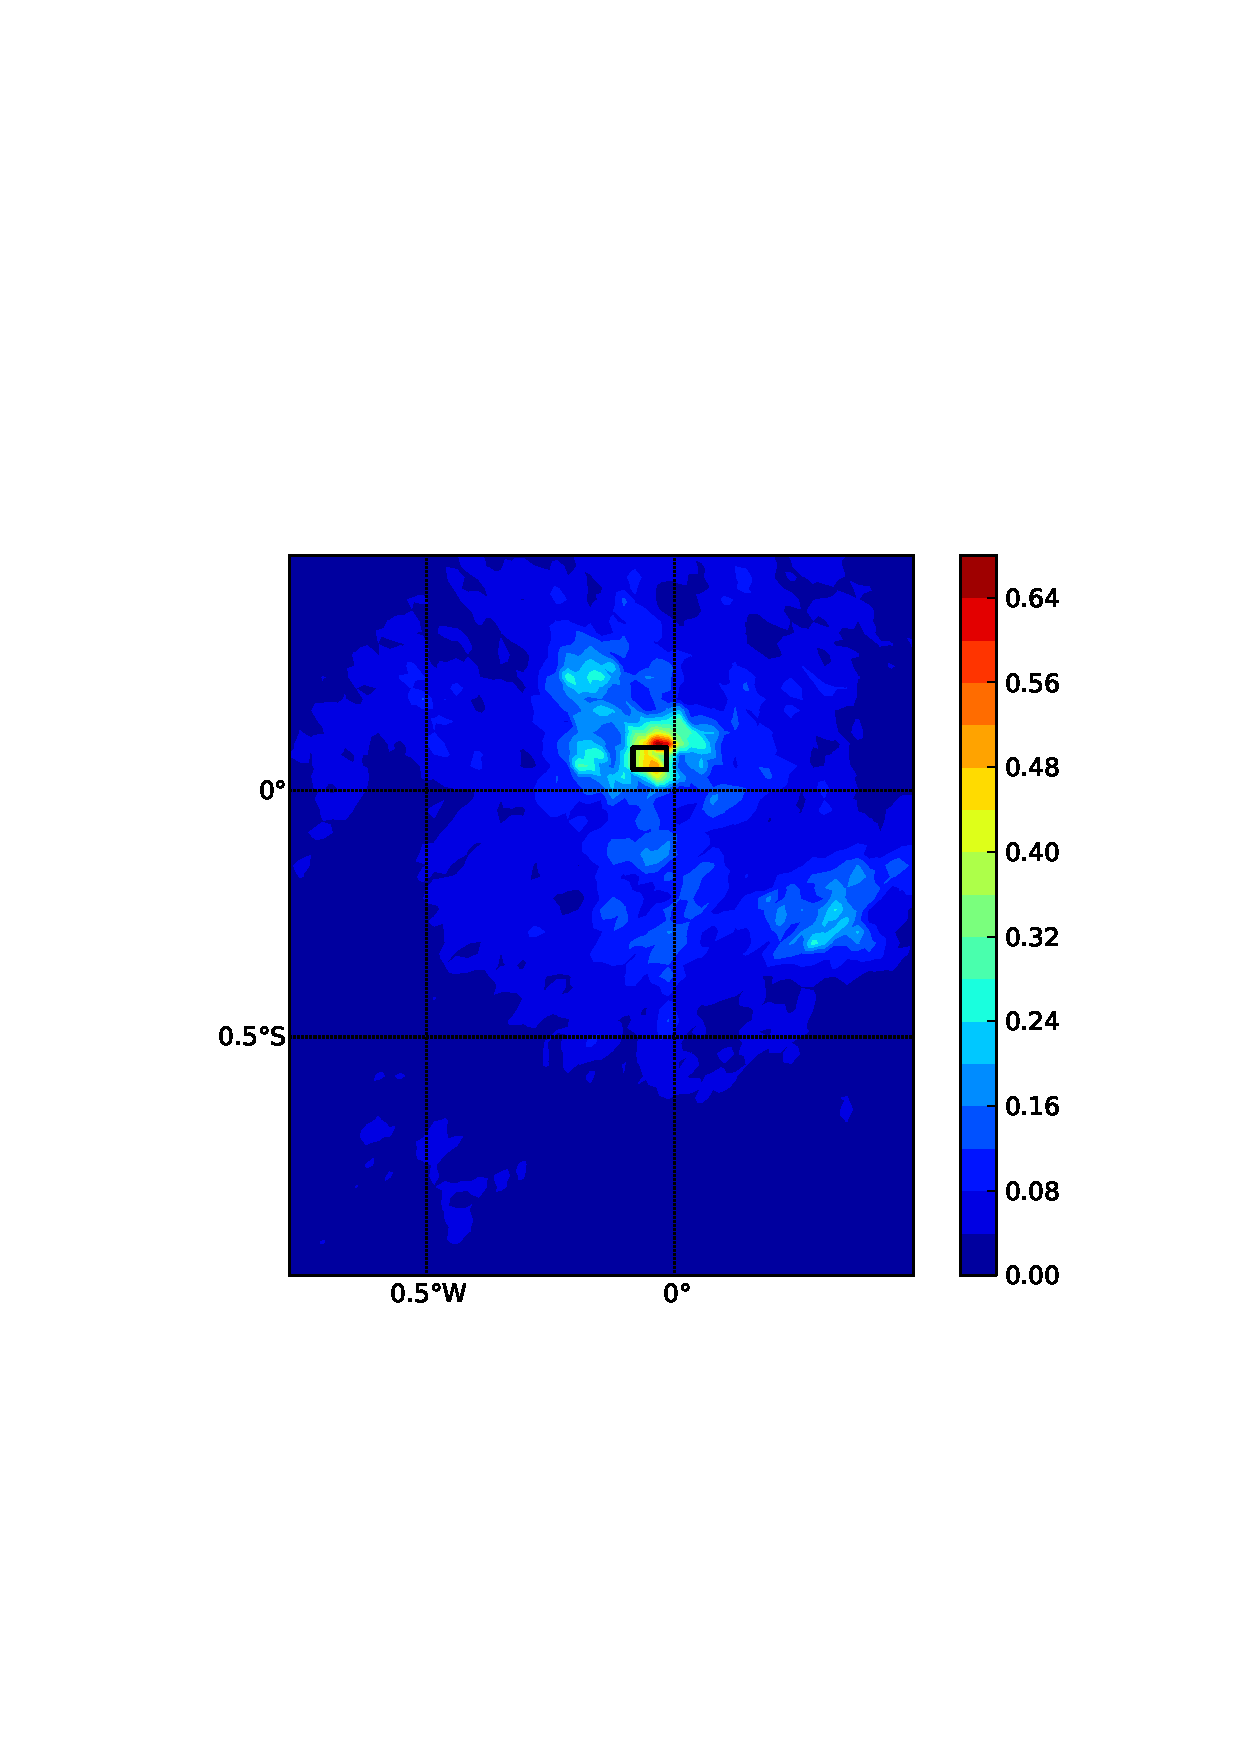
\includegraphics[width=6cm]{./figures/hazard/gmf-corr.pdf}} 
\caption{Ground motion fields (PGA) with no spatial correlations (a) and with spatial correlation (b)}
\label{fig:gmfs}
\end{figure}

\subsubsection{Disaggregation}
An example of disaggregation calculation is given considering a source model consisting of two sources (area and simple fault) belonging to two different tectonic region types.
The calculation is described by the following configuration file:
\begin{Verbatim}[frame=single, commandchars=\\\{\}, fontsize=\normalsize]
[general]

description = ...
calculation_mode = disaggregation
random_seed = 23

[geometry]

sites = 0.5 -0.5

[logic_tree]

number_of_logic_tree_samples = 0

[erf]

rupture_mesh_spacing = 2
width_of_mfd_bin = 0.1
area_source_discretization = 5.0

[site_params]

reference_vs30_type = measured
reference_vs30_value = 600.0
reference_depth_to_2pt5km_per_sec = 5.0
reference_depth_to_1pt0km_per_sec = 100.0

[calculation]

source_model_logic_tree_file = source_model_logic_tree.xml
gsim_logic_tree_file = gmpe_logic_tree.xml
investigation_time = 50.0
intensity_measure_types_and_levels = {"PGA": [...]}
truncation_level = 3
maximum_distance = 200.0

[disaggregation]

poes_disagg = 0.1
mag_bin_width = 1.0
distance_bin_width = 10.0
coordinate_bin_width = 0.2
num_epsilon_bins = 3

[output]

export_dir = ...
\end{Verbatim}
Disaggregation matrices are computed for a single site (located between the two sources) for a ground motion value corresponding to a probability value equal to 0.1
(\texttt{poes\_\-disagg = 0.1}). Magnitude values are classified in one magnitude unit bins (\texttt{mag\_\-bin\_\-width = 1.0}), distances in bins of 10 km
(\texttt{distance\_\-bin\_\-width = 10.0}), coordinates in bins of 0.2 degrees (\texttt{coordinate\_\-bin\_\-width = 0.2}). 3 epsilons bins are considered (\texttt{num\_\-epsilon\_\-bins = 3}).

\begin{comment}
The demo allows to compute 

\section{Demo 01 - Classical PSHA}

% -----------------------------------------------------------------------------
\section{Demo 02 - Classical PSHA: simple logic tree}
This demo contains simple logic tree structures accounting for epistemic
uncertainties in the seismic source and ground motion intensity models.

The seismic source model incorporates epistemic uncertainty about the 
value of the maximum magnitude of the magnitude-frequency distribution 
used.
%
The ground motion intensity model includes uncertainty about the ground
motion prediction equations to be used in the calculation of hazard.

Given that the overall structure of the logic tree is not particularly
complex and assuming that uncertainties are fully correlated we decide 
to compute all the possible realisations of the logic tree by fixing 
the \texttt{number\_\-of\_\-logic\_\-tree\_\-samples} parameter in the 
configuration file to zero.
\begin{Verbatim}[frame=single, commandchars=\\\{\}, fontsize=\normalsize]
[logic_tree]
number_of_logic_tree_samples = 0
\end{Verbatim}

Let's now run the OpenQuake:
\begin{Verbatim}[frame=single, fontsize=\normalsize]
user@ubuntu:~/demos/classical_psha_simple_lt$ oq-engine \ 
--rh job_1strike.ini 
\end{Verbatim}

This is the list of results that we get at the end of this calculation:
\begin{Verbatim}[frame=single, commandchars=\\\{\}, fontsize=\normalsize]
Calculation 8 results:
id | output_type | name
5 | hazard_curve | hc-rlz-10
6 | hazard_curve | hc-rlz-7
7 | hazard_curve | hc-rlz-8
8 | hazard_curve | hc-rlz-9
9 | hazard_curve | hc-rlz-11
10 | hazard_curve | hc-rlz-12
11 | hazard_map | hazard-map(0.1)-PGA-rlz-10
12 | hazard_map | hazard-map(0.1)-PGA-rlz-7
13 | hazard_map | hazard-map(0.1)-PGA-rlz-8
14 | hazard_map | hazard-map(0.1)-PGA-rlz-9
15 | hazard_map | hazard-map(0.1)-PGA-rlz-11
16 | hazard_map | hazard-map(0.1)-PGA-rlz-12
\end{Verbatim}
OpenQuake produced six hazard curves and six hazard maps i.e. one
result for each leaf of the logic tree. 
\end{comment}
% ==============================================================================
% ------------------------------------------------------------------------- Part
\part{Risk}
% ------------------------------------------------------------------------------
\chapter{Introduction to the risk module}
	\section{Introduction}
The seismic risk results are being calculated using the OpenQuake risk library (oq-risklib), an open-source suit of tools for seismic risk assessment and loss estimation. This library is written in the Python programming language and available in the form of a "developers" release, that can be executed through a command line interface. Its code can be found on a public repository at GitHub through the following address \href{http://gitub.com/gem/oq-risklib}{http://gitub.com/gem/oq-risklib}.

This section provides a brief description of the calculators currently implemented on riskLib, and an initial presentation of the input and output files is provided. In the following sections, the contents and structure of these files are discussed in detail. For further information regarding the methodologies behind each calculator, users are referred to the OpenQuake Book.

\section{Calculation workflows}
\label{sec:riskCalculators}
The oq-engine is currently composed by five risk calculation workflows: two that calculate losses and damage distributions due to a single earthquake, another two that calculate seismic risk using probabilistic seismic hazard, and a fifth one that uses loss exceedance curves to assess whether retrofitting measures would be economically viable or not. 

\subsection{Scenario Risk Calculator}
This calculator computes loss maps and loss statistics due to a single seismic event, for a collection of assets. The hazard input can be a single ground motion field (e.g. the median distribution of ground motion in the region of interest) or a set of ground motion fields allowing the characterisation of the inter- and intra-event variability from the GMPE. It is noted that the hazard input can either be calculated using the hazard component of OpenQuake engine (oq-hazardlib), or provided to the risk component in an external file following the respective NRML schema.
A vulnerability model is combined with the distribution of the ground motions at each asset location to calculate the loss distribution for each asset, as well as the statistics of the total loss throughout the region of interest. The required input files and resulting output files are depicted in Figure \ref{fig:ScnRisk}.

\begin{figure}[ht]
\centering
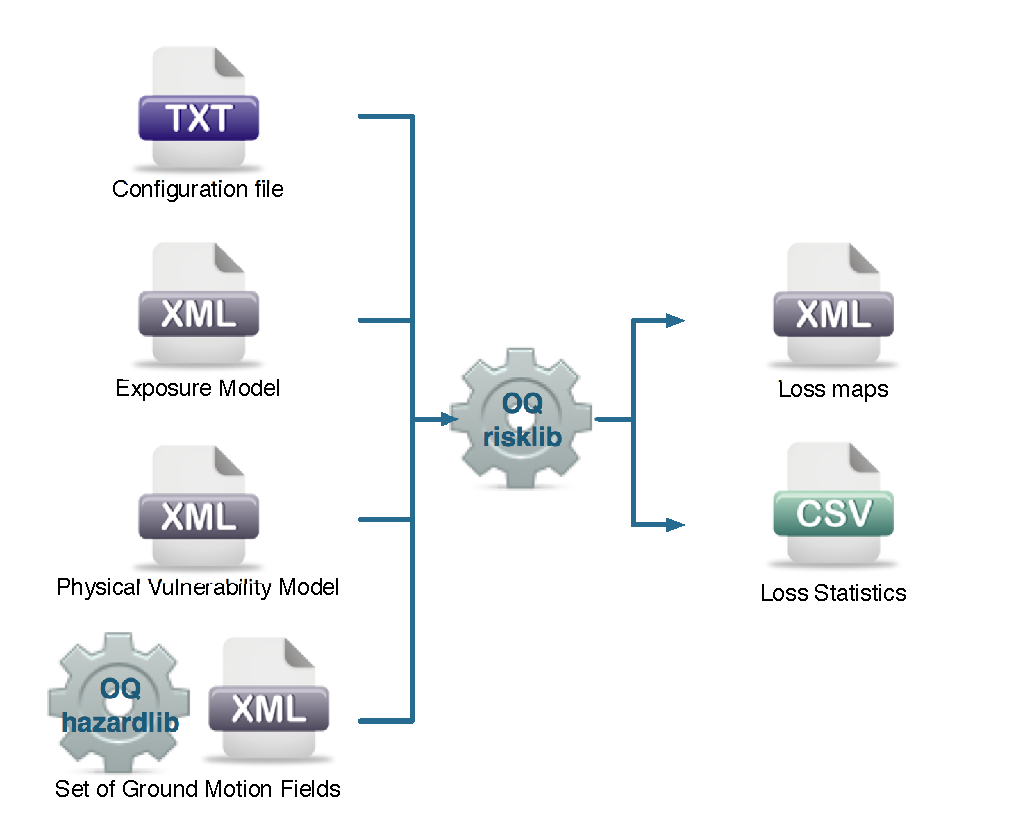
\includegraphics[width=9cm,height=7cm]{./figures/risk/ScenarioRisk.eps}
\caption{Scenario Risk Calculator input/output structure.}
\label{fig:ScnRisk}
\end{figure}

\subsection{Scenario Damage Calculator}
This calculator is capable of assessing the damage distribution due to a single scenario earthquake, for a collection of assets. Similarly to the previous calculator, in order to perform the necessary risk calculations one or a set of ground motion fields are required, which can be derived using the oq-hazardlib, or introduced in the OpenQuake engine using the appropriate NRML schema.
In this calculator, a fragility model is combined with the distribution of ground motion at the location of each asset, to estimate the number or area of buildings in each damage state. The damage distribution can be extracted per asset, per building typology (taxonomy) or considering all of the assets simultaneously (total damage distribution). In addition, this calculator also provides collapse maps, which contain the spatial distribution of the number or area of collapses throughout the region of interest. The input/output structure for this calculator is presented in Figure \ref{fig:ScnDamage}.

\begin{figure}[ht]
\centering
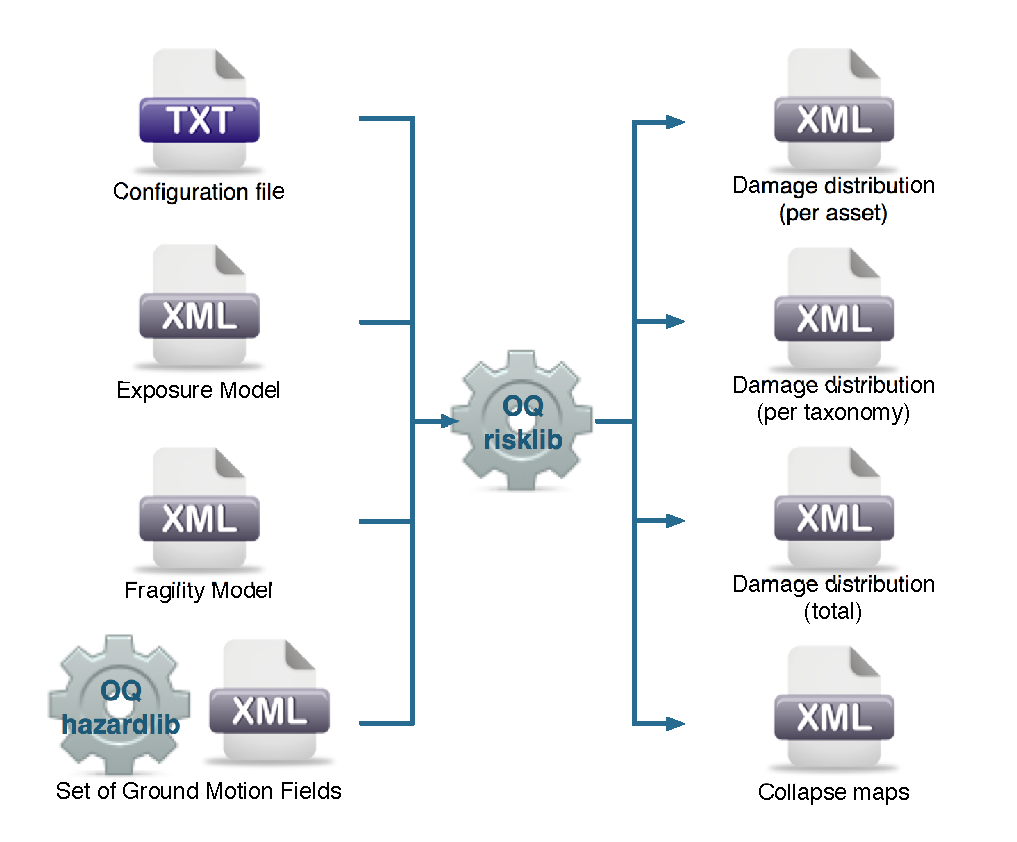
\includegraphics[width=9cm,height=7cm]{./figures/risk/ScenarioDamage.eps}
\caption{Scenario Damage Calculator input/output structure.}
\label{fig:ScnDamage}
\end{figure}

\subsection{Probabilistic Event-based Risk Calculator}
In this calculator, loss exceedance curves and loss maps for various return periods can be calculated, based on probabilistic seismic hazard, with an event-based approach. A large number of stochastic event sets are generated, and the associated ground motion fields are used together with a vulnerability model to compute the individual (per asset) and total (sum of all the losses per event) losses. Then, this distribution of losses is employed to derive a loss exceedance curve per asset, as well as a total loss exceedance curve representative of the complete building portfolio. Furthermore, oq-risklib can also compute loss maps for various return periods by interpolating each individual loss curve with the respective probability of exceedance. In Figure \ref{fig:ProbEvent}, the input/output scheme of this calculator is illustrated. 

\begin{figure}[ht]
\centering
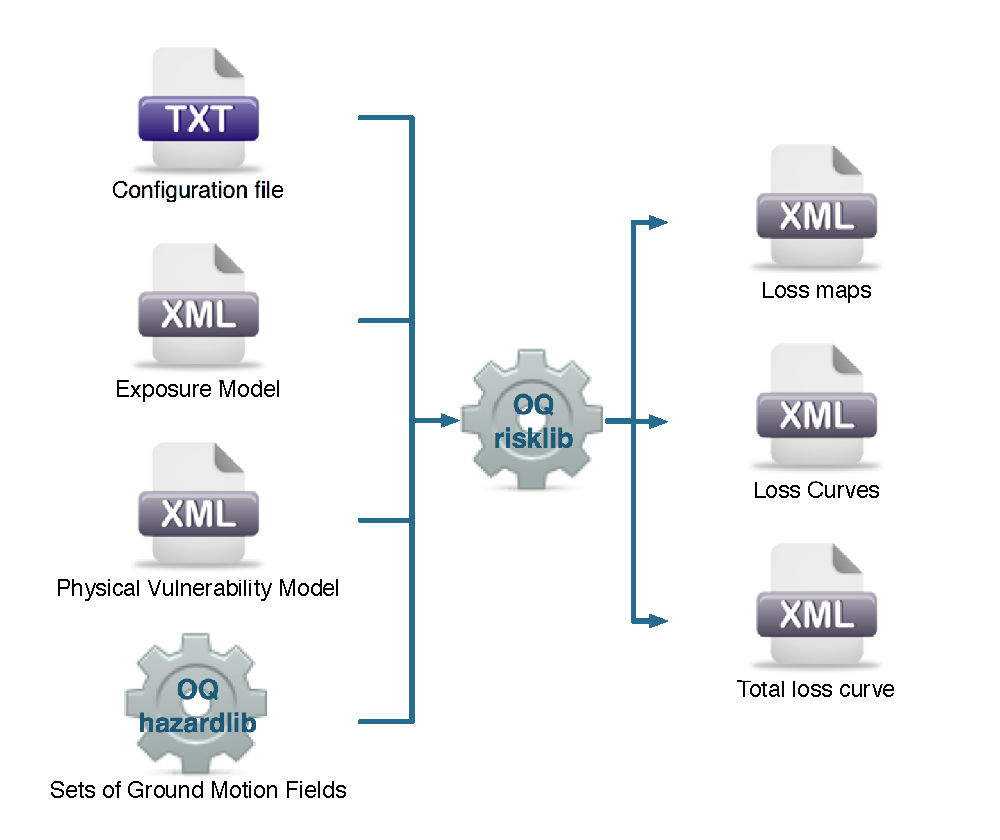
\includegraphics[width=9cm,height=7cm]{./figures/risk/ProbEvent.eps}
\caption{Probabilistic Event-based Risk Calculator input/output structure.}
\label{fig:ProbEvent}
\end{figure}

\subsection{Classical PSHA-based Risk Calculator}
In this calculator, probabilistic seismic hazard is employed to calculate a loss exceedance curve for each asset, through the usage of seismic hazard curves. A convolution between the vulnerability function and the hazard curve at location of the asset is performed, leading to the probability of exceeding a set of loss ratios. Each loss ratio is multiplied by the asset value to obtain the final loss exceedance curve. Furthermore, probabilistic loss maps can be extracted by interpolating the loss curves at each location by various probabilities of exceedance. Unlike what was described in the previous calculator, a total loss curve can not be extracted using this calculator, as the correlation of the ground motion residuals is not taken into consideration. The input and output files involved in this calculator are presented in Figure \ref{fig:ClassialPSHA}.

\begin{figure}[ht]
\centering
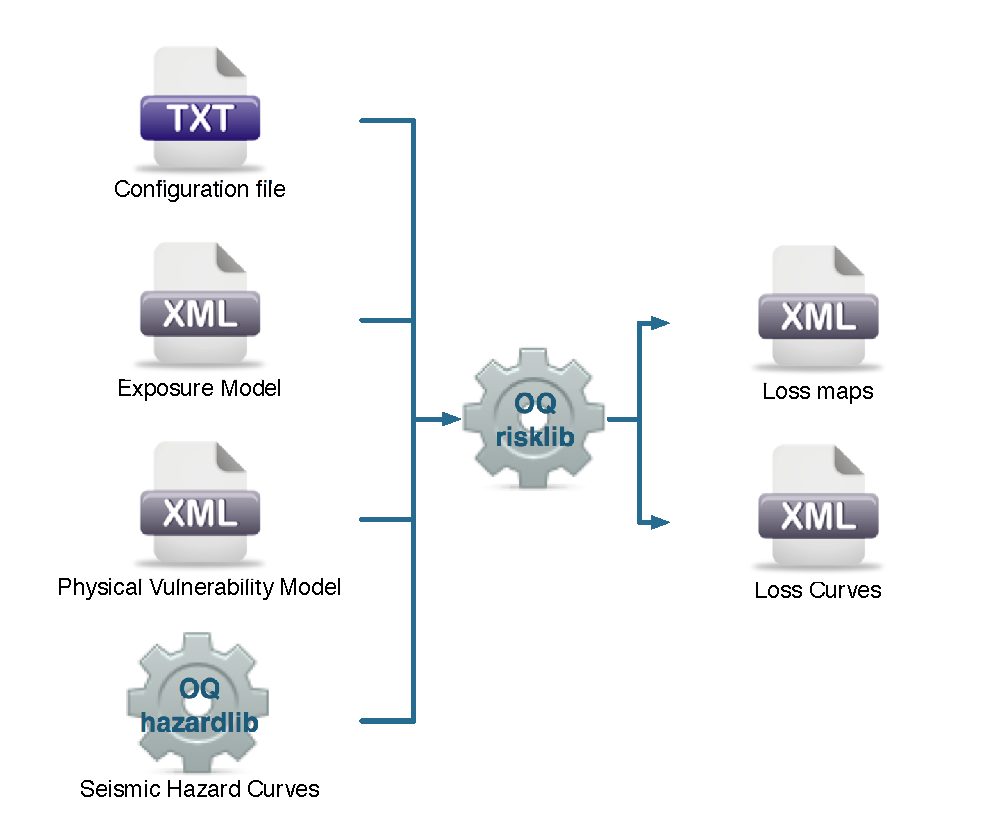
\includegraphics[width=9cm,height=7cm]{./figures/risk/ClassicalPSHA.eps}
\caption{Classical PSHA-based Risk Calculator input/output structure.}
\label{fig:ClassialPSHA}
\end{figure}

\subsection{Benefit/Cost Ratio Calculator}
This calculator represents a decision-support tool for deciding whether the employment of retrofitting measures to a collection of existing buildings is advantageous from an economical point of view. For this assessment, the expected losses considering the original and retrofitted configuration of the buildings are estimated, and the economic benefit due to the better seismic design is divided by the retrofitting cost, leading to the benefit/cost ratio. These loss curves can be computed using either the previously described Probabilistic Event-based Risk or the Classical PSHA-based Risk calculators. The output of this calculator is a benefit/cost ratio for each asset, in which a ratio above one indicates that employing  a retrofitting intervention is economically viable. In Figure \ref{fig:BCR}, the input/output structure for this calculator is depicted.

\begin{figure}[ht]
\centering
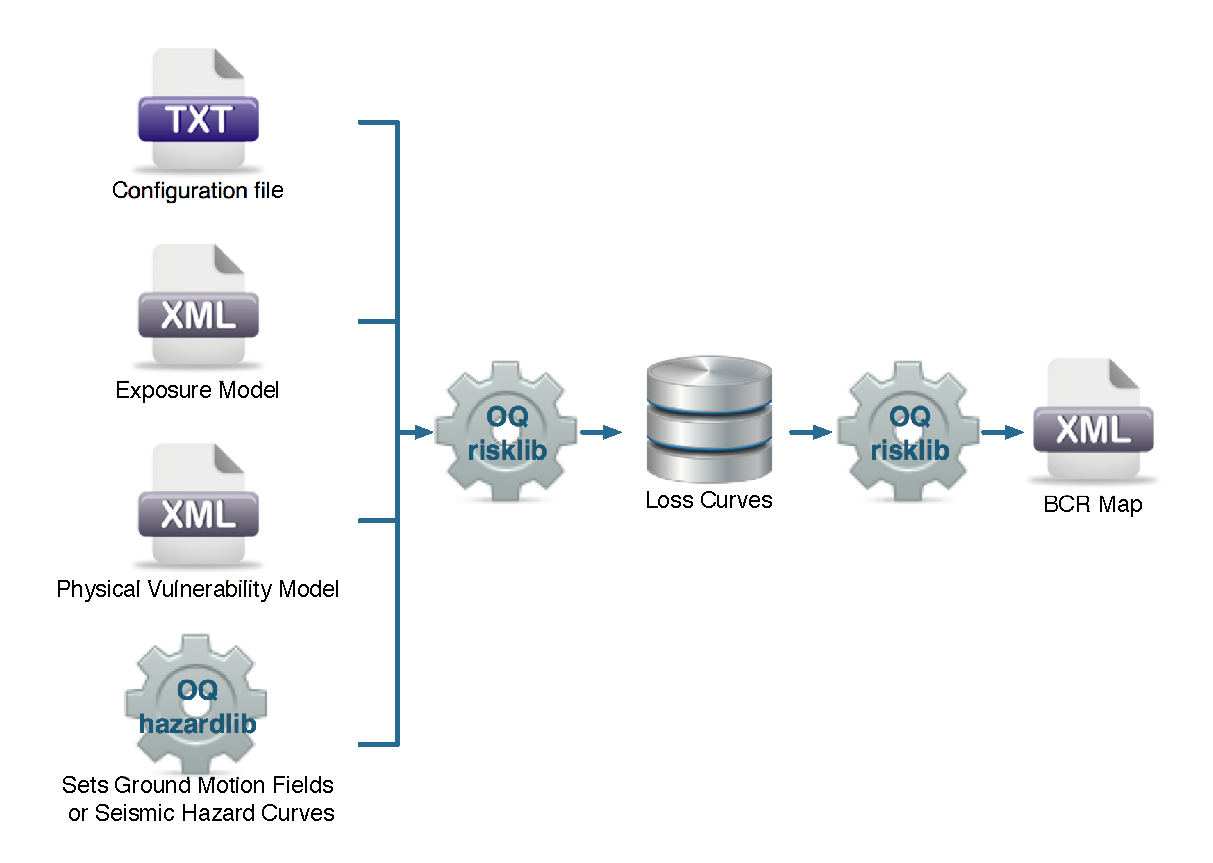
\includegraphics[width=10.5cm,height=7cm]{./figures/risk/BCR.eps}
\caption{Benefit/Cost Ratio Calculator input/output structure.}
\label{fig:BCR}
\end{figure}
% ------------------------------------------------------------------------------
\chapter{Using the risk module}
	\label{chap:riskmodule}
	\section{Input data definition}
\subsection{Exposure model definition}
All risk calculators in the OpenQuake engine require an \gls{exposure model} that needs to be stored in NRML. The following metadata, that is common to all of the \glspl{asset} stored in a given \gls{exposure model}, needs to be provided, as described below: 

\begin{itemize}
\item  \Verb+id+: a unique key used to identify the \gls{exposure model};
\item  \Verb+assetCategory+: a string used to define the type of \glspl{asset} being stored (e.g: buildings, population, contents);
\item  \Verb+areaType+: flag defining the way the area is being provided, as explained later in this section; 
\item  \Verb+areaUnits+: attribute defining the units used to measure the area; 
\item  \Verb+stcoType+: flag defining the way the structural replacement cost is being provided, as explained later in this section; 
\item  \Verb+stcoUnits+: attribute defining the units used to measure the structural replacement cost;
\item  \Verb+recoType+: flag defining the way the retrofitting cost is being provided, as explained later in this section; 
\item  \Verb+recoUnits+: attribute defining the units used to measure the retrofitting cost;
\item  \Verb+description+: brief string with further information about the \gls{exposure model};
\item  \Verb+taxonomySource+: attribute used to define the \gls{taxonomy} being used to classify the \glspl{asset};
\end{itemize}

The way the information about the characteristics of the \glspl{asset} in an \gls{exposure model} are stored can vary strongly depending on how and why the data was compiled. As an example, if national census information is used to estimated the distribution of assets in a given region, it is likely that the number of buildings within a given geographical area will be used to define the dataset, and will be used for estimating the number of collapsed buildings for a scenario earthquake. On the other hand, if simplified methodologies based on proxy data such as population distribution are used to develop the exposure model, then it is likely that the built up area or economic value of each building typology will be directly derived, and will be used for the estimation of economic losses. Thus, the following set of attributes were included in the latest version of the schema for the exposure model:

\begin{itemize}
\item  \Verb+number+: number of units of a given \gls{asset} at a given location;
\item  \Verb+area+: area of the \gls{asset}, at a given location;
\item  \Verb+stco+: structural replacement cost of the \gls{asset} at a given location; 
\item  \Verb+reco+: retrofitting cost of the \gls{asset} at a given location. 
\end{itemize}

While the attribute \Verb+number+ might be a rather simple parameter, the other two (area and cost) can be ambiguous, as different ways to define them might be used. With regards to the attribute \Verb+area+, one can either choose to provide the aggregated built up area of the \glspl{asset} per location or the average built up area for a single building unit (noting that an \gls{asset} might be made up of a number of individual buildings). Similarly, the \Verb+stco+ can also be defined as the aggregated structural replacement cost, the cost of replacing a single unit or even the structural replacement cost per unit of area. For the purposes of performing a retrofitting benefit/cost analysis, it is also necessary to define the retrofitting cost (\Verb+reco+). This parameter is being handled in the same manner as the structural replacement cost. Thus, it can be defined as the aggregated retrofitting cost, the average cost per unit of area, or as the average cost for a single building unit. 

To establish the way these three attributes are being defined within the \gls{exposure model}, three flags have been introduced in the schema model:  \Verb+areaType+, \Verb+stcoType+ and \Verb+recoType+.

Note that since the attribute \Verb+number+ always represents the same quantity (number of units of a given \gls{asset} in a given location), no flag providing further information about this attribute was introduced. Further information regarding the parameters that are currently being used to define the exposure elements can be found in the OpenQuake Engine Book (Risk). In order to clarify this methodology, several examples are presented later in this section.

Finally, a pair of coordinates (longitude and latitude) needs to be provided to define the location of each asset. The way this information is being stored is constantly being modified, as further feedback from users and experts is received. Hence, it is important to understand which version of NRML the engine is using, in order to avoid incompatibility issues. NRML is currenly v0.4 and documentation about each release can be found on GitHub (see \href{http://gitub.com/gem/oq-nrmllib}{oq-nrmllib}). Several examples of \glspl{exposure model} containing different types of information are presented below. Users will notice that some of the attributes are marked with a "\Verb+gml+" tag, which means that these parameters must follow the Geography Markup Language grammar, developed by the Open Geospatial Consortium.\

\paragraph{Example 1}
This example is comprised of an \gls{exposure model} in which the aggregated economic value of the buildings of each building typology for a set of locations is directly provided.

\begin{Verbatim}[frame=single, commandchars=\\\{\}, samepage=false]
<?xml version="1.0" encoding="UTF-8"?>
<nrml xmlns:gml="http://www.opengis.net/gml"
      xmlns="http://openquake.org/xmlns/nrml/0.4">
<\textcolor{red}{exposureModel} gml:id="ep">
    <\textcolor{green}{exposureList} gml:id="Nepal_13_1" assetCategory="buildings" 
    stcoUnit="EUR" stcoType="aggregated" recoUnit="EUR" 
    recoType="aggregated">
    <gml:description>Buildings in Nepal</gml:description>
    <taxonomySource>Nepal taxonomy</taxonomySource>
        <\textcolor{blue}{assetDefinition} gml:id="asset1">
            <site>
               <gml:Point srsName="epsg:4326">
               <gml:pos>15.22 38.80</gml:pos>
               </gml:Point>
            </site>
            <taxonomy>URM</taxonomy>
            <stco> 500.0 </stco>
            <reco> 50.0 </reco>
        <\textcolor{blue}{/assetDefinition} 
        ...
        <\textcolor{blue}{assetDefinition} gml:id="asset999">
            <site>
               <gml:Point srsName="epsg:4326">
	      <gml:pos>15.23 38.95</gml:pos>
	      </gml:Point>
	   </site>
	   <taxonomy>RC</taxonomy>
	   <stco> 700.0 </stco>
	   <reco> 70.0 </reco>
        <\textcolor{blue}{/assetDefinition}> 
    <\textcolor{green}{/exposureList}>
<\textcolor{red}{/exposureModel}>
</nrml>
\end{Verbatim}

Each \gls{asset} is uniquely identified by its \Verb+id+, which is used by the OpenQuake engine to relate each asset with the associated results (e.g. loss exceedance curves). Then, a pair of coordinates (latitude and longitude) for a \Verb+site+ is defined. This position (\Verb+pos+) and the associated geographical projection (\Verb+srsName+) need to be provided in the \Verb+Point+ attribute. Each asset must to be classified according to a \Verb+taxonomy+, so that the OpenQuake engine is capable of employing the appropriate \gls{vulnerability function} or \gls{fragility function} in the risk calculations. Finally, the structural replacement value of the asset is stored in the \Verb+stco+ attribute. In this case, the aggregated economic value for all units of a given asset at each location is provided directly, so there is no need to define other attributes such as \Verb+number+ or \Verb+area+. This mode of representing an exposure model is probably the simplest.\\ 

\paragraph{Example 2}
This example is comprised of an \gls{exposure model} containing the number of units (buildings) at each location, and the associated structrual replacement and retrofitting cost per unit of each building typology.

\begin{Verbatim}[frame=single, commandchars=\\\{\}, samepage=false]
<?xml version="1.0" encoding="UTF-8"?>
<nrml xmlns:gml="http://www.opengis.net/gml"
      xmlns="http://openquake.org/xmlns/nrml/0.4">
<\textcolor{red}{exposureModel} gml:id="ep">
    <\textcolor{green}{exposureList} gml:id="Nepal_13_2" assetCategory="buildings" 
    stcoUnit="EUR" stcoType="per_asset" recoUnit="EUR" 
    recoType="per_asset">
    <gml:description>Buildings in Nepal</gml:description>
    <taxonomySource>Nepal taxonomy</taxonomySource>
        <\textcolor{blue}{assetDefinition} gml:id="asset1">
            <site>
               <gml:Point srsName="epsg:4326">
               <gml:pos>15.22 38.80</gml:pos>
               </gml:Point>
            </site>
            <taxonomy>URM</taxonomy>
            <number> 10 </number>
            <stco> 50.0 </stco>
            <reco> 5.0 </reco>
        <\textcolor{blue}{/assetDefinition} 
        ...
        <\textcolor{blue}{assetDefinition} gml:id="asset999">
            <site>
               <gml:Point srsName="epsg:4326">
	      <gml:pos>15.23 38.95</gml:pos>
	      </gml:Point>
	   </site>
	   <taxonomy>RC</taxonomy>
            <number> 5 </number>
	   <stco> 140.0 </stco>
	   <reco> 14.0 </reco>
        <\textcolor{blue}{/assetDefinition}> 
    <\textcolor{green}{/exposureList}>
<\textcolor{red}{/exposureModel}>
</nrml>
\end{Verbatim}

In this example, the structural replacement and retrofitting value of each asset is not provided directly, as happened in the previous example. In order to carry out the risk calculations in which the structural and retrofitting value of each asset is required, the OpenQuake engine multiplies, for each asset, the number of units (buildings) by the "per unit" replacement cost. Note that in this case, there is no need to specify the attribute \Verb+area+. 

\paragraph{Example 3}
This example is comprised of an \gls{exposure model} containing the built up area of each building typology for a set of locations, and the associated structural replacement and retrofitting cost per area.

\begin{Verbatim}[frame=single, commandchars=\\\{\}, samepage=false]
<?xml version="1.0" encoding="UTF-8"?>
<nrml xmlns:gml="http://www.opengis.net/gml"
      xmlns="http://openquake.org/xmlns/nrml/0.4">
<\textcolor{red}{exposureModel} gml:id="ep">
    <\textcolor{green}{exposureList} gml:id="Nepal_13_3" assetCategory="buildings" 
    stcoUnit="EUR/m2" stcoType="per_area" recoUnit="EUR/m2" 
    recoType="per_area" areaUnit="m2" areaType="aggregated">
    <gml:description>Buildings in Nepal</gml:description>
    <taxonomySource>Nepal taxonomy</taxonomySource>
        <\textcolor{blue}{assetDefinition} gml:id="asset1">
            <site>
               <gml:Point srsName="epsg:4326">
               <gml:pos>15.22 38.80</gml:pos>
               </gml:Point>
            </site>
            <taxonomy>URM</taxonomy>
            <area> 10000 </area>
            <stco> 400.0 </stco>
            <reco> 40.0 </reco>
        <\textcolor{blue}{/assetDefinition} 
        ...
        <\textcolor{blue}{assetDefinition} gml:id="asset999">
            <site>
               <gml:Point srsName="epsg:4326">
	      <gml:pos>15.23 38.95</gml:pos>
	      </gml:Point>
	   </site>
	   <taxonomy>RC</taxonomy>
            <area> 20000 </area>
            <stco> 500.0 </stco>
            <reco> 50.0 </reco>
        <\textcolor{blue}{/assetDefinition}> 
    <\textcolor{green}{/exposureList}>
<\textcolor{red}{/exposureModel}>
</nrml>
\end{Verbatim}

Once again, the OpenQuake engine needs to carry out some calculations in order to compute the economic value per asset. In this case, this value is computed by multiplying the aggregated built up area for each building typology by the associated replacement or retrofitting cost per unit of area. Notice that in this case, there is no need to specify the attribute \Verb+number+.

 \paragraph{Example 4}
This example is comprised of an \gls{exposure model} containing the number of buildings for each location, the average built up area per building unit and the associated structural replacement and retrofitting cost per area. 

\begin{Verbatim}[frame=single, commandchars=\\\{\}, samepage=false]
<?xml version="1.0" encoding="UTF-8"?>
<nrml xmlns:gml="http://www.opengis.net/gml"
      xmlns="http://openquake.org/xmlns/nrml/0.4">
<\textcolor{red}{exposureModel} gml:id="ep">
    <\textcolor{green}{exposureList} gml:id="Nepal13_04" assetCategory="buildings" 
    stcoUnit="EUR/m2" stcoType="per_area" recoUnit="EUR/m2" 
    recoType="per_area" areaUnit="m2" areaType="per_asset">
    <gml:description>Buildings in Nepal</gml:description>
    <taxonomySource>Nepal taxonomy</taxonomySource>
        <\textcolor{blue}{assetDefinition} gml:id="asset1">
            <site>
               <gml:Point srsName="epsg:4326">
               <gml:pos>15.22 38.80</gml:pos>
               </gml:Point>
            </site>
            <taxonomy>URM</taxonomy>
            <number> 10 </number>
            <area> 100.0 </area>
            <stco> 400.0 </stco>
            <reco> 40.0 </reco>
        <\textcolor{blue}{/assetDefinition} 
        ...
        <\textcolor{blue}{assetDefinition} gml:id="asset999">
            <site>
               <gml:Point srsName="epsg:4326">
	      <gml:pos>15.23 38.95</gml:pos>
	      </gml:Point>
	   </site>
	   <taxonomy>RC</taxonomy>
            <number> 5 </number>
            <area> 150.0 </area>
            <stco> 500.0 </stco>
            <reco> 50.0 </reco>
        <\textcolor{blue}{/assetDefinition}> 
    <\textcolor{green}{/exposureList}>
<\textcolor{red}{/exposureModel}>
</nrml>
\end{Verbatim}

In this example, the OpenQuake engine will make use of all the parameters to estimate the economic and retrofitting value for each asset, by multiplying the number of buildings by its average built up area, and then by the respective replacement or retrofitting cost per unit of area. 

\paragraph{Example 5}
This example is comprised of an \gls{exposure model} containing population distribution.

\begin{Verbatim}[frame=single, commandchars=\\\{\}, samepage=false]
<?xml version="1.0" encoding="UTF-8"?>
<nrml xmlns:gml="http://www.opengis.net/gml"
      xmlns="http://openquake.org/xmlns/nrml/0.4">
<\textcolor{red}{exposureModel} gml:id="ep">
    <\textcolor{green}{exposureList} gml:id="Nepal13_5" assetCategory="population">
    <gml:description>Population in Nepal</gml:description>
    <taxonomySource>Nepal taxonomy</taxonomySource>
        <\textcolor{blue}{assetDefinition} gml:id="asset1">
            <site>
               <gml:Point srsName="epsg:4326">
               <gml:pos>15.22 38.80</gml:pos>
               </gml:Point>
            </site>
            <taxonomy>VF1</taxonomy>
            <number> 200 </number>
        <\textcolor{blue}{/assetDefinition} 
        ...
        <\textcolor{blue}{assetDefinition} gml:id="asset999">
            <site>
               <gml:Point srsName="epsg:4326">
	      <gml:pos>15.23 38.95</gml:pos>
	      </gml:Point>
	   </site>
	   <taxonomy>VF2</taxonomy>
            <number> 100 </number>
        <\textcolor{blue}{/assetDefinition}> 
    <\textcolor{green}{/exposureList}>
<\textcolor{red}{/exposureModel}>
</nrml>
\end{Verbatim}

In this final example, the OpenQuake engine will require population distribution instead of structural replacement cost, hence, only the attribute \Verb+number+ needs to be provided. Notice that in order for the engine to recognize that human losses are going to be estimated rather than economic losses, the attribute \Verb+assetCategory+ needs to be set to  \Verb+population+.  
 
Scripts capable of converting information about the assets stored in Excel or ASCII files into NRML have been developed by the scientists working at \gls{acr:gem} and can be found at the GEM Science tools repository at GitHub (\textcolor{blue01}{\Verb+http://github.com/GEMScienceTools+}). 

\subsection{Physical vulnerability model definition}
In this section, the NRML schema for the \gls{vulnerability model} is described in detail. In order to do so, a graphical representation of a \gls{vulnerability model} (mean loss ratio for a set of intensity measure levels) is illustrated in Figure \ref{fig:vulModel}, and the equivalent NRML file is then presented. Note that although the uncertainty for each loss ratio is not represented in the aforementioned figure, it has been considered in the input NRML file, by means of a coefficient of variation per loss ratio and an associated lognormal distribution. This model is comprised of two discrete \glspl{vulnerability function} and uses spectral acceleration for a given period of vibration as the intensity measure type. 

\begin{figure}[ht]
\centering
\includegraphics[width=10cm,height=6cm]{./figures/risk/vulnerabilityModel.eps}
\caption{Graphical representation of a vulnerability model.}
\label{fig:vulModel}
\end{figure}

Each component of the associated NRML file is presented herein:
 
\begin{Verbatim}[frame=single, commandchars=\\\{\}, samepage=true]
<?xml version="1.0" encoding="UTF-8"?>
<nrml xmlns:gml="http://www.opengis.net/gml"
      xmlns="http://openquake.org/xmlns/nrml/0.4">
<\textcolor{red}{vulnerabilityModel}>
    <\textcolor{green}{discreteVulnerabilitySet} vulnerabilitySetID="OpenQuake2013"	
    assetCategory="buildings"    lossCategory="economic loss">
        ...
\end{Verbatim}

At the top of the NRML schema, the following metadata are being stored:
\begin{itemize}
\item  \Verb+vulnerabilitySetID+: A unique key used to identify the \gls{vulnerability model} instance within the OpenQuake engine;
\item  \Verb+assetCategory+: An attribute that describes the asset typology (e.g.: population, buildings, contents);
\item  \Verb+lossCategory+: An attribute that describes the type of loss being modelled for the assetCategory (e.g.: fatalities, structural replacement cost, contents replacement cost). 
\end{itemize}

\begin{Verbatim}[frame=single, commandchars=\\\{\}, samepage=true]
    ...
        <\textcolor{blue}{IML}  IMT = "SA(0.3)"> 0.061 0.129 0.188 0.273 0.398 0.579 
        0.843 1.227 1.856 2.485 <\textcolor{blue}{/IML}>
        ...
\end{Verbatim}

Within this component, an attribute specifying the intensity measure type (e.g.: Sa, PGA, MMI) is defined, followed by the list of intensity measure levels. This set of values is common to all of the \glspl{vulnerability function} in the model.

\begin{Verbatim}[frame=single, commandchars=\\\{\}, samepage=true]
        ...
        <\textcolor{blue}{discreteVulnerability}  vulnerabilityFunctionID="typeA" 
        probabilisticDistribution="LN">
            <\textcolor{magenta}{lossRatio}> 0.002 0.007 0.014 0.028 0.058 0.118
            0.223 0.370 0.446 0.523 <\textcolor{magenta}{/lossRatio}>
            <\textcolor{magenta}{coefficientsVariation}> 0.012 0.058 0.079 0.159 0.265 
            0.244 0.211 0.152 0.088 0.082 <\textcolor{magenta}{/coefficientsVariation}>
        <\textcolor{blue}{/discreteVulnerability}>
        <\textcolor{blue}{discreteVulnerability}  vulnerabilityFunctionID="typeB" 
        probabilisticDistribution="LN">
            <\textcolor{magenta}{lossRatio}> 0.006 0.025 0.052 0.108 0.215 0.391	
            0.613 0.820 0.894 0.967 <\textcolor{magenta}{/lossRatio}>
            <\textcolor{magenta}{coefficientsVariation}> 0.010 0.054 0.082 0.167 0.285 
            0.278 0.261 0.132 0.084 0.021 <\textcolor{magenta}{/coefficientsVariation}>
        <\textcolor{blue}{/discreteVulnerability}>
    <\textcolor{green}{/discreteVulnerabilitySet} 
<\textcolor{red}{/vulnerabilityModel}>        
</nrml>
\end{Verbatim}

Finally, for each discrete \gls{vulnerability function} the following parameters are required:
\begin{itemize}
\item  \Verb+ vulnerabilityFunctionID +: A unique key that is used to relate each \gls{vulnerability function} with the \glspl{asset} in the \gls{exposure model};
\item  \Verb+ probabilisticDistribution +: An attribute that establishes the type of probabilistic distribution used to model the uncertainty in loss ratio. At the moment, the OpenQuake engine only supports lognormal distributions, however, other types of distributions such as beta will be incorporated in future releases;
\item  \Verb+ lossRatio +: A set of mean loss ratios (one for each intensity measure level defined previously). These values can represent different losses such as fatality rates (ratio between the number of fatalities and total population exposed) or so-called damage ratio (ratio between the repair cost and the replacement cost of a given structure).
\item  \Verb+ coefficientsVariation +: A set of coefficients of variation (one per loss ratio) that describes the uncertainty in the loss ratio. If users do not want to consider the uncertainty, this set of parameters can be set to zero, and the OpenQuake engine assumes each loss ratio as a deterministic value. 
\end{itemize}

In the previously described \gls{vulnerability model} all of the \glspl{vulnerability function} were defined in terms of a single intensity measure type (Sa for 0.3 seconds). However, the current version of the engine also allows the employment of a \gls{vulnerability model} that is comprised of \glspl{vulnerability function} that each use distinct intensity measure types. In the following example, the schema of a \gls{vulnerability model} in which three intensity measure types were used (PGA, PGV and Sa for 0.3 seconds) is presented.

\begin{Verbatim}[frame=single, commandchars=\\\{\}, samepage=false]
<?xml version="1.0" encoding="UTF-8"?>
<nrml xmlns:gml="http://www.opengis.net/gml"
      xmlns="http://openquake.org/xmlns/nrml/0.4">
<\textcolor{red}{vulnerabilityModel}>
    <\textcolor{green}{discreteVulnerabilitySet} vulnerabilitySetID="Nepal13_PGA"
    assetCategory="buildings"    lossCategory="economic loss">
        <\textcolor{blue}{IML}  IMT = "PGA"> 0.1 0.2 0.4 0.7 1.0 1.3 <\textcolor{blue}{/IML}>
       <\textcolor{blue}{discreteVulnerability}  vulnerabilityFunctionID="RC1" 
        probabilisticDistribution="LN">
            <\textcolor{magenta}{lossRatio}> 0.02 0.1 0.3 0.6 0.8 0.9 <\textcolor{magenta}{/lossRatio}>
            <\textcolor{magenta}{coefficientsVariation}> 0.7 0.5 0.3 0.2 0.1 0.05 
            <\textcolor{magenta}{/coefficientsVariation}>
        <\textcolor{blue}{/discreteVulnerability}>
    <\textcolor{green}{/discreteVulnerabilitySet} 
    <\textcolor{green}{discreteVulnerabilitySet} vulnerabilitySetID="Nepal13_PGV"
    assetCategory="buildings"    lossCategory="economic loss">
        <\textcolor{blue}{IML}  IMT = "PGV"> 5 20 40 60 80 100 <\textcolor{blue}{/IML}>
       <\textcolor{blue}{discreteVulnerability}  vulnerabilityFunctionID="RC2" 
        probabilisticDistribution="LN">
            <\textcolor{magenta}{lossRatio}> 0.05 0.2 0.3 0.4 0.5 0.6 <\textcolor{magenta}{/lossRatio}>
            <\textcolor{magenta}{coefficientsVariation}> 0.6 0.3 0.2 0.1 0.05 0.05 
            <\textcolor{magenta}{/coefficientsVariation}>
        <\textcolor{blue}{/discreteVulnerability}>
    <\textcolor{green}{/discreteVulnerabilitySet} 
    <\textcolor{green}{discreteVulnerabilitySet} vulnerabilitySetID="Nepal13_SA"
    assetCategory="buildings"    lossCategory="economic loss">
        <\textcolor{blue}{IML}  IMT = "SA(0.3)"> 0.1 0.3 0.6 0.9 1.2 1.5 <\textcolor{blue}{/IML}>
       <\textcolor{blue}{discreteVulnerability}  vulnerabilityFunctionID="RC3" 
        probabilisticDistribution="LN">
            <\textcolor{magenta}{lossRatio}> 0.01 0.06 0.12 0.17 0.24 0.33 <\textcolor{magenta}{/lossRatio}>
            <\textcolor{magenta}{coefficientsVariation}> 1.5 1.1 1.0 0.9 0.8 0.5 
            <\textcolor{magenta}{/coefficientsVariation}>
        <\textcolor{blue}{/discreteVulnerability}>
    <\textcolor{green}{/discreteVulnerabilitySet} 
<\textcolor{red}{/vulnerabilityModel}>  
</nrml>      
\end{Verbatim}

Several methodologies to derive vulnerability functions are currently being evaluated by \gls{acr:gem} and will be a part of a set of modelling tools. Scripts to convert \glspl{vulnerability function} stored in Excel or ASCII files into NRML have already being developed, and can be found at the GEM Science tools repository at GitHub (\textcolor{blue01}{\Verb+http://github.com/GEMScienceTools+}).

\subsection{Fragility model definition}
This section describes the schema currently used to store \glspl{fragility model}, which are required for the Scenario Damage Calculator. A \gls{fragility model} can be comprised of several \glspl{fragility function}, describing the probability of exceeding a set of limit, or damage, states. These \glspl{fragility function} can be defined in two ways: discrete or continuous. In the former manner, sets of probabilities of exceedance (one set per limit state) are defined for a list of intensity measure levels, as illustrated in Figure \ref{fig:fragModelDiscrete}. 

\begin{figure}[ht]
\centering
\includegraphics[width=8cm,height=6cm]{./figures/risk/DisFragilityModel.eps}
\caption{Graphical representation of a discrete fragility model.}
\label{fig:fragModelDiscrete}
\end{figure}

Similarly to what has been described for the \glspl{vulnerability model}, the NRML schema for this input also has some attributes that are common to all of the \glspl{fragility function} comprising the model. This initial portion of the schema is depicted below:

\begin{Verbatim}[frame=single, commandchars=\\\{\}, samepage=true]
<?xml version="1.0" encoding="UTF-8"?>
<nrml xmlns:gml="http://www.opengis.net/gml"
      xmlns="http://openquake.org/xmlns/nrml/0.4">
<\textcolor{red}{<fragilityModel format="discrete">}>
    <\textcolor{green}{description} "Fragility Model for RC" <\textcolor{green}{/description}>
    <\textcolor{green}{limitStates} 
        slight damage
        moderate damage
        collapse     
    <\textcolor{green}{/limitStates}>
    ...
\end{Verbatim}

\begin{itemize}
\item  \Verb+description+: represents an attribute that can be used to include  some information about the \gls{fragility model}, for example, what building typologies are being covered or the source of the \gls{fragility model};
\item  \Verb+limitStates+: this field is used to define the number and nomenclature of each limit state. Despite the fact that three limit states are being employed in this example, it is possible to use any number of states, as long as a fragility curve is always defined for each limit state. 
\end{itemize}
    
\begin{Verbatim}[frame=single, commandchars=\\\{\}, samepage=true]
    ...  
    <\textcolor{green}{ffs noDamageLimit= 0.05}> 
        <\textcolor{blue}{taxonomy} RC <\textcolor{blue}{/taxonomy}>
        <\textcolor{blue}{IML} IMT="PGA" imlUnit="g"> 0.0 0.25 0.50 0.75 1.00 <\textcolor{blue}{/IML}>
        
        <\textcolor{blue}{ffd} ls="slight damage">
            <\textcolor{magenta}{poes}> 0.0 0.85 0.98 0.99 1.00 < \textcolor{magenta}{/poes}>
        <\textcolor{blue}{/ffd}
        <\textcolor{blue}{ffd} ls="moderate damage">
            <\textcolor{magenta}{poes}> 0.0 0.32 0.75 0.91 0.97 < \textcolor{magenta}{/poes}>
        <\textcolor{blue}{/ffd}
        <\textcolor{blue}{ffd} ls="collapse">
            <\textcolor{magenta}{poes}> 0.0 0.07 0.37 0.64 0.80 < \textcolor{magenta}{/poes}>
        <\textcolor{blue}{/ffd}      
    <\textcolor{green}{/ffs}> 
<\textcolor{red}{/fragilityModel}>  
</nrml>      
\end{Verbatim}

For each building typology, a set of limit state curves need to be stored within the field \Verb+ffs+ (fragility function set). The following attributes are currently being employed to define this input:

\begin{itemize}
\item  \Verb+noDamageLimit+: this attribute defines the intensity measure level below which the probability of exceedance for all curves is zero;  
\item  \Verb+taxonomy+: a unique key that is used to relate each \gls{fragility function} with the relevant \glspl{asset} in the \gls{exposure model}; 
\item  \Verb+IML+: this attribute serves the purposes of defining the list of intensity measure levels for which the limit state curves are defined. In addition, it is also necessary to define the intensity measure type (\Verb+IMT+) being used and the respective units (\Verb+imlUnit+);
\item  \Verb+ffd+: this field (fragility function discrete) is used to define the probabilities of exceedance (\Verb+poes+) of each limit state curve. It is also necessary to include which limit state is being defined in the attribute \Verb+ls+.
\end{itemize}

As previously mentioned, the user may choose to define the \glspl{fragility function} in a continuous manner, through the use of cumulative lognormal functions. In Figure \ref{fig:fragModelContinuous}, a continuous fragility model is presented.

\begin{figure}[ht]
\centering
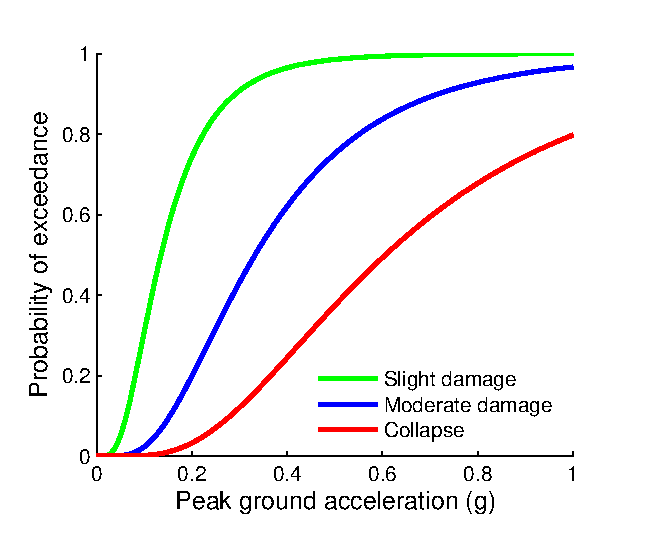
\includegraphics[width=8cm,height=6cm]{./figures/risk/ConFragilityModel.eps}
\caption{Graphical representation of a continuous fragility model.}
\label{fig:fragModelContinuous}
\end{figure}

The NRML schema to store these functions has an initial structure similar to that described for the discrete \glspl{fragility model}. Then, the continuous limit state curves are stored as illustrated below:

\begin{Verbatim}[frame=single, commandchars=\\\{\}, samepage=true]
    ...  
    <\textcolor{green}{ffs noDamageLimit= 0.05}> 
        <\textcolor{blue}{taxonomy} RC <\textcolor{blue}{/taxonomy}>
        <\textcolor{blue}{IML} IMT="PGA" minIML="0.0" maxIML="1.0" imlUnit="g" ><\textcolor{blue}{/IML}>
        <\textcolor{blue}{ffd} ls="slight damage">
            <params \textcolor{magenta}{mean}="0.16" \textcolor{magenta}{stddev}="0.11" />
        <\textcolor{blue}{/ffd}
        <\textcolor{blue}{ffd} ls="moderate damage">
            <params \textcolor{magenta}{mean}="0.40" \textcolor{magenta}{stddev}="0.26" />
        <\textcolor{blue}{/ffd}
        <\textcolor{blue}{ffd} ls="collapse">
            <params \textcolor{magenta}{mean}="0.73" \textcolor{magenta}{stddev}="0.48" />
        <\textcolor{blue}{/ffd}      
    <\textcolor{green}{/ffs}> 
<\textcolor{red}{/fragilityModel}>
</nrml>        
\end{Verbatim}

Again, the set of limit state curves for each building typology needs to be stored within the field \Verb+ffs+ (fragility function set), through the definition of the following attributes:

\begin{itemize}
\item  \Verb+noDamageLimit+: this attribute defines the intensity measure level below which the probability of exceedance for all curves is zero;
\item  \Verb+type+: this parameter defines the type of probabilistic distribution being used to define the limit state curves. Currently the engine only supports lognormal distributions, however, the capability of considering other types of distributions (e.g. normal, exponential) will be developed in the future;
\item  \Verb+taxonomy+: a unique key that is used to relate each \gls{fragility function} with the relevant \glspl{asset} in the \gls{exposure model};  
\item  \Verb+IML+: in this field, the intensity measure type (\Verb+IMT+) and associated units (\Verb+imlUnit+) for the limit state curves is defined, along with the minimum (\Verb+minIML+) and maximum (\Verb+maxIML+) intensity measure levels enclosing the range of applicability of the set of fragility functions;
\item  \Verb+ffc+: this field (fragility function continuous) is used to define the mean (\Verb+mean+) and standard deviation (\Verb+stddev+) of the cumulative lognormal function. In addition, the limit state for the curve being defined needs to be specified in the attribute \Verb+ls+.
\end{itemize}

\subsection{Configuration file}
The configuration file (or job.ini file) represents the location where the paths to the input files, the parameters controlling the risk calculations and the type of outputs are defined. Some initial parameters common to all the risk calculators are presented below. The remaining parameters that are specific to each risk calculator are discussed in subsequent sections. For additional information about how each parameter is being used within the methodologies implemented in the oq-engine, users advised to consult the OpenQuake Engine Book (Risk). 

\begin{Verbatim}[frame=single, commandchars=\\\{\}, samepage=true]
[general]
description = Scenario Risk Nepal
calculation_mode = scenario

exposure_file = exposure_model.xml
region_constraint = 78.0 31.5,89.5 31.5,89.5 25.5,78 25.5
maximum_distance = 10
...
\end{Verbatim}

\begin{itemize}
\item  \Verb+description+: a parameter that can be used to include some information about the type of calculations that are going to be performed;
\item  \Verb+calculation_mode+: this parameter sets the type of calculations. The key word for each risk calculator is described in the following sections;
\item  \Verb+exposure_file+: this parameter is used to specify the path to the \gls{exposure model} file;
\item  \Verb+region_constraint+: this field is used to define the polygon enclosing the region of interest. Assets outside of this region will not be considered in the risk calculations. This region is defined using pairs of coordinates (longitude and latitude in decimal degrees) that indicate the vertexes of the polygon;
\item  \Verb+maximum_distance+: this parameter indicates the maximum allowable distance between an \gls{asset} and the closest hazard input. If no hazard input is found within this distance, the \gls{asset} is skipped and a message is provided mentioning the id of the asset that is affected by this issue.
\end{itemize}

Depending on the type of calculations, other parameters besides the aforementioned ones need to be provided, as will be described in the following sections.

\subsubsection{Scenario Risk Calculator}
In order to run this calculator, the parameter \Verb+calculation_mode+ needs to be set to \Verb+scenario+. The remaining parameters are illustrated bellow.

\begin{Verbatim}[frame=single, commandchars=\\\{\}, samepage=true]
...
vulnerability_file = vulnerability_model.xml
asset_correlation = 0.7
master_seed = 3
\end{Verbatim}

\begin{itemize}
\item  \Verb+vulnerability_file+: this parameter is used to specify the path to the \gls{vulnerability model} file;
\item  \Verb+asset_correlation+: if the uncertainty in the loss ratios has been defined within the \gls{vulnerability model}, users can specify a coefficient of correlation that will be used in the Monte Carlo sampling process of the loss ratios, between the assets that share the same \gls{taxonomy}. If the \Verb+asset_correlation+ is set to one, the loss ratio residuals will be perfectly correlated. On the other hand, if this parameter is set to zero, the loss ratios will be sampled independently. Any value between zero and one will lead to increasing levels of correlation;
\item  \Verb+master_seed+: this parameter is used to control the random generator in the loss ratio sampling process. This way, if the same \Verb+master_seed+ is defined at each calculation run, the same random loss ratios will be generated, thus allowing replicability of the results.
\end{itemize}

\subsubsection{Scenario Damage Calculator}
For this calculator, the parameter \Verb+calculation_mode+ needs to be defined as \Verb+scenario_damage+. There is only one parameter specific to this calculator, which is the \gls{fragility model} file path, as presented below.

\begin{Verbatim}[frame=single, commandchars=\\\{\}, samepage=true]
...
fragility_file = fragility_model.xml
\end{Verbatim}

\begin{itemize}
\item  \Verb+fragility_file+: a parameter used to define the path to the \gls{fragility model} file.
\end{itemize}

\subsubsection{Probabilistic Event-based Risk Calculator}
The parameter \Verb+calculation_mode+ needs to be set to \Verb+event_based+ in order to use this calculator. Similarly to that described for the Scenario Risk Calculator, a Monte Carlo sampling process is also employed within this module to take into account the loss ratio uncertainty. Hence, the parameters \Verb+asset_correlation+ and \Verb+master_seed+ need to be defined as previously described. The remaining parameters are presented below.

\begin{Verbatim}[frame=single, commandchars=\\\{\}, samepage=true]
...
vulnerability_file = vulnerability_model.xml
asset_correlation = 0.7
master_seed = 3

loss_curve_resolution = 20
conditional_loss_poes = 0.01, 0.05, 0.1
\end{Verbatim}

\begin{itemize}
\item  \Verb+loss_curve_resolution+: since this calculator uses an event-based approach, a large number of levels of loss (and associated probabilities of exceedance) is computed (one per event) for each asset. The oq-risklib will use this large set of results to extrapolate a loss curve, whose number of points are controlled by this parameter;
\item  \Verb+conditional_loss_poes+: this parameter is used to define the probabilities of exceedance at which loss maps are to be produced.
\end{itemize}

\subsubsection{Classical PSHA-based Risk Calculator}
In order to run this calculator, the parameter \Verb+calculation_mode+ needs to be set to \Verb+classical+. With this calculator it is also possible to extract loss maps, so the parameter \Verb+conditional_loss_poes+ needs to be defined as explained in the previous sub-section. The remaining parameter is illustrated below.
\begin{Verbatim}[frame=single, commandchars=\\\{\}, samepage=true]
...
vulnerability_file = vulnerability_model.xml

lrem_steps_per_interval = 2
conditional_loss_poes = 0.01, 0.05, 0.1
\end{Verbatim}

\begin{itemize}
\item  \Verb+lrem_steps_per_interval+: this parameter controls the number of intermediate values between consecutive loss ratios (as defined in the \gls{vulnerability model}) that are considered in the risk calculations. A larger number of loss ratios than those defined in each \gls{vulnerability function} should be considered, in order to better account for the uncertainty in the loss ratio distribution. More details are provided in the OpenQuake Engine Book (Risk).  
\end{itemize}

\subsubsection{Retrofitting Benefit/Cost Ratio Calculator}
As previously explained, this calculator uses loss exceedance curves which can be calculated using the Classical PSHA-based Risk or the Probabilistic Event-based Risk calculators. Therefore, depending on which calculator a user chooses to employ, the configuration file will be different. If the Classical PSHA-based Risk calculator is employed, then the \Verb+calculation_mode+ should be set to \Verb+classical_bcr+ and the calculator-specific part of the configuration file should be defined as presented below.

\begin{Verbatim}[frame=single, commandchars=\\\{\}, samepage=true]
...
vulnerability_file = vulnerability_model.xml
vulnerability_retrofitted_file = vulnerability_model_retrof.xml

lrem_steps_per_interval = 2

interest_rate= 0.005
asset_life_expectancy = 50
\end{Verbatim}

\begin{itemize}
\item  \Verb+vulnerability_retrofitted_file+: this parameter is used to specify the path to the \gls{vulnerability model} file containing the \glspl{vulnerability function} for the retrofitted assets;  
\item  \Verb+interest_rate+: this parameter represents the interest rate and it serves the purposes of taking into account the variation of building value throughout time;
\item  \Verb+asset_life_expectancy+: this variable defines the life expectancy, or design life, of the assets.
\end{itemize}

Alternatively, if a user decides to employ the Probabilistic Event-based Risk calculator for the calculation of the loss curves, then the \Verb+calculation_mode+ should be set to \Verb+event_based_bcr+ and the remaining portion of the configuration file should be defined as follows.

\begin{Verbatim}[frame=single, commandchars=\\\{\}, samepage=true]
...
vulnerability_file = vulnerability_model.xml
vulnerability_retrofitted_file = vulnerability_model_retrof.xml
asset_correlation = 0.7
master_seed = 3

loss_curve_resolution = 20

interest_rate= 0.005
asset_life_expectancy = 50
\end{Verbatim}
% ------------------------------------------------------------------------------
\chapter{Risk calculations and results}	
	\label{chap:riskout}
	\section{Running OpenQuake engine for risk calculations}
Using the command line interface, risk calculations can be launched and the resulting outputs can be extracted. This section describes all the currently implemented commands and presents examples for each of the calculators.
One of the first tasks that needs to be performed is the definition of the seismic hazard input. As mentioned in section \ref{sec:riskCalculators}, the risk calculations can use the results produced by the hazard component of the OpenQuake engine. Moreover, for the two scenario-based calculators, users also have the option of loading a set of ground motion fields that might have been produced using the OpenQuake engine, or other software.
In order to load ground motion fields based on a single earthquake event, it is fundamental to ensure that the ground motion values have been stored according to the appropriate NRML schema, as presented in section \ref{EventBasedOutput}. Then, the following command can be used:

\begin{Verbatim}[frame=single, commandchars=\\\{\}, samepage=true]
user@ubuntu:~\$ oq-engine --loadgmf <gml_directory>
\end{Verbatim}

Whether a user chooses to load pre-computed ground motion fields, or calculate this input using the hazard component of the OpenQuake engine, a unique \verb+id+ is associated to the set of ground motion fields, as depicted below.

\begin{Verbatim}[frame=single, commandchars=\\\{\}, samepage=true]
Calculation 3 results:
id | output_type | name
12 | gmf_scenario | gmf_scenario
\end{Verbatim}

This is the parameter that will be used when launching the risk calculations to indicate which hazard input should be employed. In the case of the scenario-based calculators, there is only a single hazard input (one or a set of ground motion fields). For the remaining calculators, where probabilistic seismic hazard is used, it is possible to have multiple hazard inputs due to the employment of logic trees, as described in section \ref{sec:hazInputData}. In the following illustration, a set of hazard results produced using the Classical PSHA calculator is presented.

\begin{Verbatim}[frame=single, commandchars=\\\{\}, samepage=true]
Calculation 4 results:
id | output_type | name
32 | hazard_curve | hc-rlz-32-PGA
33 | hazard_curve | hc-rlz-33-PGA
34 | hazard_curve | hc-rlz-34-PGA
35 | hazard_curve | hc-rlz-35-PGA
36 | hazard_curve | mean curve for PGA
37 | hazard_curve | quantile curve (poe>= 0.15) for imt PGA
38 | hazard_curve | quantile curve (poe>= 0.85) for imt PGA
\end{Verbatim}

In this case, since the logic tree had four branches, fours sets of hazard curves were produced, each one with its own \verb+id+. In addition, mean and quantile hazard curves were also produced. A user may choose to run risk calculations using results from one of the branches or mean/quantile curves. To do so, the id of the respective hazard result should be employed when launching the risk calculations, as depicted below.

\begin{Verbatim}[frame=single, commandchars=\\\{\}, samepage=true]
user@ubuntu:~\$ oq-engine --run-risk job.ini --hazard-output-id
<hazard_output_id>
\end{Verbatim}

or simply:

\begin{Verbatim}[frame=single, commandchars=\\\{\}, samepage=true]
user@ubuntu:~\$ oq-engine --rr job.ini --ho <hazard_output_id>
\end{Verbatim}

On the other hand, a user might also want to run the risk calculations considering all the hazard results from a certain calculation run. In this case, rather than providing the \verb+hazard-output-id+, users need to provide the id of the hazard calculation as follows.

\begin{Verbatim}[frame=single, commandchars=\\\{\}, samepage=true]
user@ubuntu:~\$ oq-engine --run-risk job.ini --hazard-calculation-id
<hazard_calculation_id>
\end{Verbatim}

or simply:

\begin{Verbatim}[frame=single, commandchars=\\\{\}, samepage=true]
user@ubuntu:~\$ oq-engine --rr job.ini --co <hazard_calculation_id>
\end{Verbatim}

For further information about consulting the \verb+id+ of hazard results or calculations, users are referred to section \ref{sec:riskCalculators}. To obtain a list of all the risk calculations, the following command can be employed.

\begin{Verbatim}[frame=single, commandchars=\\\{\}, samepage=true]
user@ubuntu:~\$ oq-engine --list-risk-calculations
\end{Verbatim}

or simply:

\begin{Verbatim}[frame=single, commandchars=\\\{\}, samepage=true]
user@ubuntu:~\$ oq-engine --lrc
\end{Verbatim}

Which will display a list of risk calculations as presented below.

\begin{Verbatim}[frame=single, commandchars=\\\{\}, samepage=true]
calc_id | num_jobs | latest_job_status | last_update | description
1 | 1 | successful | 2013-04-02 08:50:30  | Scenario Damage
2 | 1 | failed | 2013-04-03 09:56:17  | Scenario Risk
3 | 1 | successful | 2013-04-04 10:45:32  | Scenario Risk
4 | 4 | successful | 2013-04-04 10:48:33  | Classical PSHA Risk
\end{Verbatim}

Then, in order to display a list of the risk outputs from a given job, the following command can be used

\begin{Verbatim}[frame=single, commandchars=\\\{\}, samepage=true]
user@ubuntu:~\$ oq-engine --list-risk-outputs <risk_calculation_id>
\end{Verbatim}

or simply:

\begin{Verbatim}[frame=single, commandchars=\\\{\}, samepage=true]
user@ubuntu:~\$ oq-engine --lro <risk_calculation_id>
\end{Verbatim}

Which will display a list of risk calculations as presented below.

\begin{Verbatim}[frame=single, commandchars=\\\{\}, samepage=true]
Calculation 4 results:
id | output_type | name
29 | loss_curve | loss curves. type=structural, hazard=32
30 | loss_map | loss maps. type=structural poe=0.1, hazard=32
\end{Verbatim}


Then, in order to export the risk calculation outputs in the appropriate xml format, the following command can be used.

\begin{Verbatim}[frame=single, commandchars=\\\{\}, samepage=true]
user@ubuntu:~\$ oq-engine --export-risk <risk_output_id>
<output_directory>
\end{Verbatim}

or simply:

\begin{Verbatim}[frame=single, commandchars=\\\{\}, samepage=true]
user@ubuntu:~\$ oq-engine --er <risk_output_id> <output_directory>
\end{Verbatim}

\section{Description of the outputs}
This section describes how the different risk outputs are being stored using the Natural Hazards risk Markup Language (NRML). For each output, the various attributes are discussed, and example schema is provided.

\subsection{Loss statistics}
This output is produced by the Scenario Risk calculator and is comprised by a mean total loss and associated standard deviation. These results are stored in a comma separate value (.csv) file as follows:

\begin{Verbatim}[frame=single, commandchars=\\\{\}, samepage=true]
Mean,Standard Deviation
8717775315.66,2047771108.36
\end{Verbatim}

\subsection{Loss maps}
A loss map contains the spatial distribution of the losses throughout the region of interest. This result can be produced by the Scenario Risk calculator (representing the losses from a single event), or from the Probabilistic Event-based Risk or Classical PSHA-based Risk calculators (representing the expected losses from probabilistic seismic hazard). In the former case, the loss map is comprised of a mean loss and respective standard deviation for each \gls{asset}, whilst for the latter, a single value is provided, representing the expected loss for a given return period (or probability of exceedance for a certain time span, or investigation interval). In the following example, a loss map due to a single earthquake is presented.

\begin{Verbatim}[frame=single, commandchars=\\\{\}, samepage=false]
\textcolor{gray}{<?xml version="1.0" encoding="UTF-8"?>}
<nrml xmlns:gml="http://www.opengis.net/gml"
      xmlns="http://openquake.org/xmlns/nrml/0.4">
<\textcolor{red}{lossMap} lossCategory="buildings" unit="EUR">
     <\textcolor{green}{node}>
          <gml:Point>
            <gml:pos>83.31 29.46</gml:pos>
          </gml:Point>
          \textcolor{blue}{loss} assetRef="a1" mean="53.3" stdDev="109.25"/>
          \textcolor{blue}{loss} assetRef="a2" mean="386.0" stdDev="695.7"/>
          \textcolor{blue}{loss} assetRef="a3" mean="303.1" stdDev="447.4"/>
          \textcolor{blue}{loss} assetRef="a4" mean="298.9" stdDev="453.7"/>
     <\textcolor{green}{/node}>
    ...
     <\textcolor{green}{node}>
          <gml:Point>
            <gml:pos>83.33 28.71</gml:pos>
          </gml:Point>
          \textcolor{blue}{loss} assetRef="a997" mean="277.3" stdDev="100.8"/>
          \textcolor{blue}{loss} assetRef="a998" mean="219.6" stdDev="123.5"/>
          \textcolor{blue}{loss} assetRef="a999" mean="576.3" stdDev="210.9"/>
     <\textcolor{green}{/node}>
<\textcolor{red}{/lossMap}>
</nrml>
\end{Verbatim}

\begin{itemize}
\item  \Verb+lossCategory+: the type of losses that are being stored. This parameter is taken from the \gls{vulnerability model} that was used in the loss calculations (e.g. fatalities, economic loss);
\item  \Verb+unit+: this attribute is used to define the units in which the losses are being measured (e.g. EUR);
\item  \Verb+node+: each loss map is comprised by various nodes, each node possibly containing a number of \glspl{asset}. The location of the node is defined by a latitude and longitude in decimal degrees within the field \Verb+gml:Point+. The mean loss (\Verb+mean+) and associated standard deviation (\Verb+stdDev+) for each \gls{asset} (identified by the parameter \Verb+assetRef+) is stored in the \Verb+loss+ field.
\end{itemize}

For the probabilistic loss maps (expected losses for a given return period), a set of additional parameters need to be considered as depicted in the following example.

\begin{Verbatim}[frame=single, commandchars=\\\{\}, samepage=false]
\textcolor{gray}{<?xml version="1.0" encoding="UTF-8"?>}
<nrml xmlns:gml="http://www.opengis.net/gml"
      xmlns="http://openquake.org/xmlns/nrml/0.4">
<\textcolor{red}{lossMap} investigationTime="50" poE="0.1" sourceModelTreePath="b1"
        gsimTreePath="b1" lossCategory="buildings" unit="EUR">
     <\textcolor{green}{node}>
          <gml:Point>
            <gml:pos>83.31 29.46</gml:pos>
          </gml:Point>
          \textcolor{blue}{loss} assetRef="a1" value="696.1"/>
          \textcolor{blue}{loss} assetRef="a2" value="4201.4"/>
          \textcolor{blue}{loss} assetRef="a3" value="2666.0"/>
          \textcolor{blue}{loss} assetRef="a4" value="1291.8"/>
     <\textcolor{green}{/node}>
    ...
     <\textcolor{green}{node}>
          <gml:Point>
            <gml:pos>83.33 28.71</gml:pos>
          </gml:Point>
          \textcolor{blue}{loss} assetRef="a997" value="4077.3"/>
          \textcolor{blue}{loss} assetRef="a998" value="2466.4"/>
          \textcolor{blue}{loss} assetRef="a999" value="4434.5"/>
     <\textcolor{green}{/node}>
<\textcolor{red}{/lossMap}>
</nrml>
\end{Verbatim}

\begin{itemize}
\item  \Verb+investigationTime+: time span used to compute the probability of exceedance;
\item  \Verb+poE+: parameter specifying the probability of exceedance (e.g. 0.1);
\item  \Verb+sourceModelTreePath+: this is a parameter indicating the path used to create the seismic source model;
\item  \Verb+gsimTreePath+: this parameter designates the ground motion model;
\item  \Verb+node+: this attribute follows an identical structure as seen in the previous example, but only a single loss (\Verb+value+) is provided per \gls{asset}.
\end{itemize}

\subsection{Damage distribution}
The damage distribution is part of the outputs from the Scenario Damage calculator, and can be provided in three ways: per \gls{asset}, per taxonomy or the total damage distribution. In the following illustration, an example of the NRML schema for the damage distribution per \gls{asset} is presented: 

\begin{Verbatim}[frame=single, commandchars=\\\{\}, samepage=false]
\textcolor{gray}{<?xml version="1.0" encoding="UTF-8"?>}
<nrml xmlns:gml="http://www.opengis.net/gml"
      xmlns="http://openquake.org/xmlns/nrml/0.4">
<\textcolor{red}{dmgDistPerAsset}>
     <\textcolor{green}{damageStates}>
         no_damage
         slight
         moderate
         complete
     <\textcolor{green}{/damageStates}>
     <\textcolor{green}{DDNode}>
          <gml:Point>
            <gml:pos>83.31 29.46</gml:pos>
          </gml:Point>
          <\textcolor{blue}{asset} assetRef="a1">
            <damage ds="no_damage" mean="486.6" stddev="130.1"/>
            <damage ds="slight" mean="118.8" stddev="9.9"/>
            <damage ds="moderate" mean="130.3" stddev="20.3"/>
            <damage ds="complete" mean="186.5" stddev="90.8"/>
          <\textcolor{blue}{/asset}>
          <\textcolor{blue}{asset} assetRef="2">
            <damage ds="no_damage" mean="877.08" stddev="257.9"/>
            <damage ds="slight" mean="171.3" stddev="13.2"/>
            <damage ds="moderate" mean="161.5" stddev="014.5"/>
            <damage ds="complete" mean="563.8" stddev="223.6"/>
          <\textcolor{blue}{/asset}>
     <\textcolor{green}{/DDNode}>
     ...
     <\textcolor{green}{DDNode}>
          <gml:Point>
            <gml:pos>83.91 28.19</gml:pos>
          </gml:Point>
          <\textcolor{blue}{asset} assetRef="999">
            <damage ds="no_damage" mean="21.5" stddev="16.6"/>
            <damage ds="slight" mean="15.5" stddev="8.7"/>
            <damage ds="moderate" mean="39.1" stddev="17.3"/>
            <damage ds="complete" mean="493.5" stddev="53.1"/>
          <\textcolor{blue}{/asset}>
     <\textcolor{green}{/DDNode}>
<\textcolor{red}{/dmgDistPerAsset}>
</nrml>
\end{Verbatim}

\begin{itemize}
\item  \Verb+damageStates+: this field serves the purposes of storing the set of damage states, as defined in the \gls{fragility model} employed in the calculations;
\item  \Verb+DDNode+: this attribute is used to store the damage distribution of a number of \glspl{asset}, at a given location (defined within the attribute \Verb+gml:Point+). For each \gls{asset}, the mean number of buildings (\Verb+mean+) and associated standard deviation (\Verb+stddev+) in each damage state is defined.
\end{itemize}

The Scenario Damage calculator can also estimate the total number of buildings with a certain \gls{taxonomy}, in each damage state. This  distribution of damage per building \gls{taxonomy} is depicted in the following example.

\begin{Verbatim}[frame=single, commandchars=\\\{\}, samepage=false]
\textcolor{gray}{<?xml version="1.0" encoding="UTF-8"?>}
<nrml xmlns:gml="http://www.opengis.net/gml"
      xmlns="http://openquake.org/xmlns/nrml/0.4">
<\textcolor{red}{dmgDistPerAsset}>
     <\textcolor{green}{damageStates}>
         no_damage
         slight
         moderate
         complete
     <\textcolor{green}{/damageStates}>
     <\textcolor{green}{DDNode}>
      <taxonomy>W</taxonomy>
      <damage ds="no_damage" mean="456450.2" stddev="26376.62"/>
      <damage ds="slight" mean="88102.3" stddev="3283.9"/>
      <damage ds="moderate" mean="103564.6" stddev="3487.1"/>
      <damage ds="complete" mean="275891.1" stddev="26676.8"/>
     <\textcolor{green}{/DDNode}>
     ...
     <\textcolor{green}{DDNode}>
      <taxonomy>RC</taxonomy>
      <damage ds="no_damage" mean="4484.2" stddev="460.9"/>
      <damage ds="slight" mean="932.4" stddev="106.7"/>
      <damage ds="moderate" mean="1691.7" stddev="177.9"/>
      <damage ds="complete" mean="7659.5" stddev="799.3"/>
     <\textcolor{green}{/DDNode}>
<\textcolor{red}{/dmgDistPerAsset}>
</nrml>
\end{Verbatim}

In the damage distribution per \gls{taxonomy}, each \Verb+DDNode+ contains the statistics of the number of buildings in each damage state, belonging to a given building class as specified in the \Verb+taxonomy+ attribute.
Finally, a total damage distribution can also be calculated, which contains the mean and standard deviation of the total number of buildings in each damage state, as illustrated bellow.

\begin{Verbatim}[frame=single, commandchars=\\\{\}, samepage=false]
\textcolor{gray}{<?xml version="1.0" encoding="UTF-8"?>}
<nrml xmlns:gml="http://www.opengis.net/gml"
      xmlns="http://openquake.org/xmlns/nrml/0.4">
<\textcolor{red}{totalDmgDist}>
     <\textcolor{green}{damageStates}>
         no_damage
         slight
         moderate
         complete
     <\textcolor{green}{/damageStates}>
     <\textcolor{green}{damage} ds="no_damage" mean="456450.2" stddev="26376.62"/>
     <\textcolor{green}{damage} ds="slight" mean="88102.3" stddev="3283.9"/>
     <\textcolor{green}{damage} ds="moderate" mean="103564.6" stddev="3487.1"/>
     <\textcolor{green}{damage} ds="complete" mean="275891.1" stddev="26676.8"/>
<\textcolor{red}{/totalDmgDist}>
</nrml>
\end{Verbatim}

\subsection{Collapse maps}
Collapse maps are part of the Scenario Damage calculator outputs. These results provide the spatial distribution of the number of the collapsed buildings throughout the area of interest. An example of the schema is presented below.

\begin{Verbatim}[frame=single, commandchars=\\\{\}, samepage=false]
\textcolor{gray}{<?xml version="1.0" encoding="UTF-8"?>}
<nrml xmlns:gml="http://www.opengis.net/gml"
      xmlns="http://openquake.org/xmlns/nrml/0.4">
<\textcolor{red}{collapseMap}>
     <\textcolor{green}{CMNode}>
          <gml:Point>
            <gml:pos>83.31 29.46</gml:pos>
          </gml:Point>
          <\textcolor{blue}{cf} assetRef="a1" mean="227.1" stdDev="95.8"/>
          <\textcolor{blue}{cf} assetRef="a2" mean="703.2" stdDev="240.2"/>
          <\textcolor{blue}{cf} assetRef="a3" mean="199.5" stdDev="63.3"/>
          <\textcolor{blue}{cf} assetRef="a4" mean="357.8" stdDev="136.1"/>
     <\textcolor{green}{/CMNode}>
    ...
     <\textcolor{green}{CMNode}>
          <gml:Point>
            <gml:pos>83.33 28.71</gml:pos>
          </gml:Point>
          <\textcolor{blue}{cf} assetRef="a997" mean="239.4" stdDev="102.0"/>
          <\textcolor{blue}{cf} assetRef="a998" mean="733.0" stdDev="253.2"/>
          <\textcolor{blue}{cf} assetRef="a999" mean="207.4" stdDev="66.5"/>
     <\textcolor{green}{/CMNode}>
<\textcolor{red}{/collapseMap}>
</nrml>
\end{Verbatim}

This schema follows the same structure of the loss maps presented previously. Thus, the results for a number of \glspl{asset} at a given location are stored within the field \Verb(+CMNode+). This field is associated with a location (defined within the \Verb+gml:Point+ attribute) and it contains the mean number of collapses (\Verb+mean+) and respective standard deviation (\Verb+stdDev+) for each \gls{asset} (identified by the parameter \Verb+assetRef+).

\subsection{Loss exceedance curves}
Loss exceedance curves can be calculated using the Classical PSHA-based Risk or Probabilistic Event-based Risk calculators, and they provide the probability of exceeding a set of levels of loss, within a given time span (or investigation interval). Similarly to what has been described for the probabilistic loss maps, also here it is necessary to define the parameters \Verb+investigationTime+, \Verb+sourceModelTreePath+, \Verb+gsimTreePath+ and \Verb+unit+. Then, the set of loss exceedance curves are stored as presented in the following example.

\begin{Verbatim}[frame=single, commandchars=\\\{\}, samepage=false]
\textcolor{gray}{<?xml version="1.0" encoding="UTF-8"?>}
<nrml xmlns:gml="http://www.opengis.net/gml"
<\textcolor{red}{lossCurves} investigationTime="50" sourceModelTreePath="b1"
    gsimTreePath="b1" unit="EUR">
     <\textcolor{green}{lossCurve} assetRef="a1">
          <gml:Point>
            <gml:pos>83.31 29.46</gml:pos>
          </gml:Point>
          <\textcolor{blue}{poE}> 0.970 0.297 0.137 0.019 0.005 0.001</\textcolor{blue}{poE}>
          <\textcolor{blue}{losses}> 235 477 989 4102 7444 15631</\textcolor{blue}{losses}>
          <\textcolor{blue}{lossRatios}> 0.02 0.03 0.06 0.26 0.48 1.0</\textcolor{blue}{lossRatios}>
     <\textcolor{green}{/lossCurve}>
     ...
     <\textcolor{green}{lossCurve} assetRef="a999">
          <gml:Point>
            <gml:pos>83.33 28.71</gml:pos>
          </gml:Point>
          <\textcolor{blue}{poE}> 0.99 0.714 0.112 0.020 0.004 0.001</\textcolor{blue}{poE}>
          <\textcolor{blue}{losses}>58 402 819 3664 8001 13540</\textcolor{blue}{losses}>
          <\textcolor{blue}{lossRatios}> 0.02 0.04 0.07 0.32 0.59 1.0</\textcolor{blue}{lossRatios}>
     <\textcolor{green}{/lossCurve}>
<\textcolor{red}{/lossCurves}>
</nrml>
\end{Verbatim}

Each \Verb+lossCurve+ is associated with a location (defined within the \Verb+gml:Point+ attribute) and a reference to the \gls{asset} (\Verb+assetRef+) whose loss is being represented. Then, three lists of values are stored: the probabilities of exceedance (\Verb+poE+), levels of absolute loss (\Verb+losses+) and percentages of loss (\Verb+lossRatios+).

\subsection{Retrofitting Benefit/cost ratio maps}
Ratio maps from the Retrofitting Benefit/Cost Ratio calculator require loss exceedance curves, which can be calculated using the Classical PSHA-based Risk or Probabilistic Event-based Risk calculators. For this reason, the parameters \Verb+sourceModelTreePath+ and \Verb+gsimTreePath+ are also included in this NRML schema, so the whole calculation process can be tracked back. The results for each \gls{asset} are being stored as depicted below.

\begin{Verbatim}[frame=single, commandchars=\\\{\}, samepage=false]
\textcolor{gray}{<?xml version="1.0" encoding="UTF-8"?>}
<nrml xmlns:gml="http://www.opengis.net/gml"
      xmlns="http://openquake.org/xmlns/nrml/0.4">
<\textcolor{red}{bcrMap} interestRate="0.05" assetLifeExpectancy="50.0"
    sourceModelTreePath="b1" gsimTreePath="b1" unit="EUR">
     <\textcolor{green}{node}>
          <gml:Point>
            <gml:pos>83.31 29.46</gml:pos>
          </gml:Point>
          <\textcolor{blue}{bcr} assetRef="a1" ratio="1.96" aalOrig="1466.9"
              aalRetr="253.0"/>
          <\textcolor{blue}{bcr} assetRef="a2" ratio="2.33" aalOrig="937.9"
              aalRetr="215.7"/>
          <\textcolor{blue}{bcr} assetRef="a3" ratio="1.32" aalOrig="492.0"
              aalRetr="83.7"/>
          <\textcolor{blue}{bcr} assetRef="a4" ratio="0.76" aalOrig="294.1"
              aalRetr="57.9"/>
     <\textcolor{green}{/node}>
    ...
     <\textcolor{green}{node}>
          <gml:Point>
            <gml:pos>83.33 28.71</gml:pos>
          </gml:Point>
          <\textcolor{blue}{bcr} assetRef="a997" ratio="0.84" aalOrig="18323.1"
              aalRetr="7340.7"/>
          <\textcolor{blue}{bcr} assetRef="a998" ratio="1.36" aalOrig="152027.6"
              aalRetr="29123.5"/>
          <\textcolor{blue}{bcr} assetRef="a999" ratio="0.83" aalOrig="60727.3"
              aalRetr="12676.1"/>
     <\textcolor{green}{/node}>
<\textcolor{red}{/bcrMap}>
</nrml>
\end{Verbatim}

\begin{itemize}
\item  \Verb+interestRate+: this parameter represents the inflation rate of the economic value of the \glspl{asset};
\item  \Verb+assetLifeExpectancy+: a parameter specifying the life expectancy (or design life) of the \glspl{asset} considered for the calculations;
\item  \Verb+node+: this schema follows the same \Verb+node+ structure already presented for the loss maps, however, instead of losses for each \gls{asset}, the benefit/cost ratio (\Verb+ratio+), the average annual loss considering the original vulnerability (\Verb+aalOrig+) and the average annual loss for the retrofitted (\Verb+aalRetr+) configuration  of the \glspl{asset} are provided.
\end{itemize}

\subsection{Loss disaggregation}
Currently the loss disaggregation can only be performed using the Probabilistic Event-based Risk calculator. Thus, the parameters \Verb+sourceModelTreePath+ and \Verb+gsimTreePath+ have been included in the NRML schema. Additional information can also be comprised such as the \Verb+investigationTime+, \Verb+lossCategory+ and \Verb+unit+ of the losses. The OpenQuake-engine can perform loss disaggregation in terms of magnitude/distance or latitude/longitude. An example of the former type of output is presented below.

\begin{Verbatim}[frame=single, commandchars=\\\{\}, samepage=false]
\textcolor{gray}{<?xml version="1.0" encoding="UTF-8"?>}
<nrml xmlns:gml="http://www.opengis.net/gml"
      xmlns="http://openquake.org/xmlns/nrml/0.4">
<\textcolor{red}{lossFraction} investigationTime ="50.00" sourceModelTreePath="b1"
  gsimTreePath="b1" lossCategory="buildings" unit="EUR"
  variable="magnitude_distance">
    <\textcolor{green}{map}>
      <\textcolor{blue}{node} lon="85.07916667" lat="27.4625">
        <bin value="5.00,5.50|220.00,240.0000"
          absoluteLoss="150000" fraction="0.75"/>
        <bin value="6.50,7.00|480.00,500.0000"
          absoluteLoss="50000" fraction="0.25"/>
      <\textcolor{green}{/node}>
    ...
      <\textcolor{blue}{node} lon="85.67" lat="27.58">
        <bin value="5.00,5.50|220.00,240.00"
          absoluteLoss="100000" fraction="0.50"/>
        <bin value="6.50,7.00|480.00,500.00"
          absoluteLoss="50000" fraction="0.25"/>
        <bin value="7.00,7.50|350.00,370.00"
          absoluteLoss="50000" fraction="0.25"/>
      <\textcolor{green}{/node}>
<\textcolor{red}{/map}>
</nrml>
\end{Verbatim}

\begin{itemize}
\item  \Verb+variable+: The type of disaggregation is defined by this attribute, and it can assume the value \Verb+magnitude_distance+ or \Verb+coordinate+;
\item  \Verb+bin+: Each \Verb+bin+ is identified by edges of the corresponding pair of parameter that it represents (e.g. lower and upper bounds of a given combination of magnitude and distance, as illustrated in the previous example). Then, the aggregated losses associated with this pair of parameters are stored in the field \Verb+absoluteLoss+, and their percentage with respect to the overall loss are defined on the field \Verb+fraction+.
\end{itemize}

\subsection{Event loss tables}
Unlike what was described for the other outputs, the event loss tables are exported using a coma separated value (.csv) file format. In this structure, each row contains the rupture id, magnitude and aggregated loss (sum of the losses from the collection of assets within the region of interest), for each event within the stochastic event sets. The following example depicts an example of this output.

\begin{Verbatim}[frame=single, commandchars=\\\{\}, samepage=false]
Rupture,Magnitude,Aggregate Loss
1,8.25,79197
2,8.25,74478
3,7.75,46458
4,7.75,45153
5,7.75,42569
6,8.25,40649
7,7.75,38868
8,7.75,37707
9,7.75,37141
...
\end{Verbatim}
%
\chapter{Demonstrative examples}
	\label{chap:riskexamples}
	This sections describes the set of demos that have been compile to exercise the OpenQuake engine. These demos can be found in a public repository in GitHub at the following link \href{http://github.com/gem/oq-engine/tree/master/demos}{http://github.com/gem/oq-engine/tree/master/demos}. Furthermore, a folder containing all of these demonstrative examples is provided when an OATS (OpenQuake Alpha Testing Service) account is requested, and it is also part of the OpenQuake engine virtual image package. These examples are purely demonstrative and do not intend to represent accurately the seismicity, vulnerability or exposure characteristics of the region of interest, but simply to provide example input files that can be used as a benchmark for users planning to employ OpenQuake in Seismic Risk and Loss Estimation studies.  

The five demos use Nepal as the region of interest. An example exposure model has been developed for this region, comprising 9144 assets distributed amongst 2221 locations (due to the existence of more than an asset at the same location). A map with the distribution of the number of buildings throughout Nepal is presented in Figure \ref{fig:expNepal}. 

\begin{figure}[ht]
\centering
\includegraphics[width=12cm,height=8cm]{./figures/risk/NepalExposure.eps}
\caption{Distribution of number of buildings in Nepal.}
\label{fig:expNepal}
\end{figure}

The building portfolio was organised into four classes for the rural areas (adobe, dressed stone, unreinforced fired brick, wooden frames), and five classes for the urban areas (the aforementioned typologies, in addition to reinforced concrete buildings). For each one of this building typologies, a vulnerability and fragility functions was collected from the literature. These input models are only for demonstrative purposes and for further information about the building characteristics of Nepal, users are advices to contact the National Society for Earthquake Technology of Nepal (NSET - \href{http://www.nset.org.np/}{http:www.nset.org.np/}).

This section includes instruction not just to run the risk calculations, but also how to produce the necessary hazard input. Thus, each demo comprises the configuration file, exposure model and fragility/vulnerability models fundamental for the risk calculations, but also a configuration file and associated input models to produce the hazard input.

\section{Scenario Risk demo}

\section{Scenario Damage demo}

\section{Classical PSHA-based Risk demo}

\section{Probabilistic Event-based demo}

\section{Benefit/cost ratio demo}

% ==============================================================================
% ------------------------------------------------------------------------- Part
%\part{Modeller's Toolkit}
% ------------------------------------------------------------------------------
%\chapter{Introduction}
%	\glsdesc{acr:oqe} is the seismic hazard and risk calculation software developed by
the \glsdesc{acr:gem}. By following current standards in software
developments like test-driven development and continuous integration, the
\glsdesc{acr:oqe} aims at becoming an open, and community-driven tool for
seismic hazard and risk analysis.

The source code of the \glsdesc{acr:oqe} is available on a public web-based
repository at the following address:

\href{http://github.com/gem/oq-engine}{http://github.com/gem/oq-engine}.


% ------------------------------------------------------------------------------
\section{Running the OpenQuake-engine}
\index{Running OpenQuake!introduction}
\label{sec:running_oq_engine}

An \gls{acr:oqe} analysis is launched from the command line of a terminal.

A schematic list of the options that can be used for the execution of the
\gls{acr:oqe} can be obtained with the following command:

\begin{minted}[fontsize=\footnotesize,frame=single,bgcolor=lightgray]{shell-session}
user@ubuntu:~\$ oq-engine --help
\end{minted}

The result is the following:

\inputminted[firstline=1,fontsize=\footnotesize,frame=single]{shell-session}{oqum/help.txt}\\

% ------------------------------------------------------------------------------
\section{Concurrent Computing with OpenQuake}
\label{sec:concurrent_tasks}

The \glsdesc{acr:oqe} supports concurrent computing on both standalone
computers and computer clusters.

The \glsdesc{acr:oqe} works by splitting a computation into a number of tasks
which are then processed in parallel. The user has the ability to control the
splitting procedure, at least to a certain extent, by setting the parameter
`concurrent\_tasks` in the job.ini file. The \glsdesc{acr:oqe} will try to
produce a number of tasks close to `concurrent\_tasks`: it could be more, it
could be less. The details of the algorithm used can change depending on the
release of the engine and this is why they are not documented here. Instead,
we will document how you can set the parameter to a sensible value.

For instance, suppose you have a standard PC with an i7 processor with 8
hyperthreaded cores, i.e. 4 real cores. You could set:

concurrent\_tasks = 16

and then each hyperthreaded core would process around 2 tasks, which is a
reasonable value. If your computation consumes a lot of memory, you could
increase `concurrent\_tasks`, thus producing more tasks of smaller size,
requiring less memory.

If you don't set the parameter, a default value is used. Currently the default
is set to 8 times the number of cores in your controller machine. This default
value for `concurrent\_tasks` is likely to change in the future and you should
not rely on it if you are using a computer cluster. If you are not using a
cluster, the default value should be a reasonable choice.

Now, suppose you have have a cluster with a controller node and 10 workers,
each of which has 8 hyperthreaded cores, making for 80 cores in total. In this
scenario you could set:

concurrent\_tasks = 160

If you did not set the parameter, the default (assuming 8 cores on the
controller machine) would be 8 * 8 = 64 tasks, which is not enough. The number
of available cores on the workers is 80, so 16 cores will remain unused. Our
suggestion is to provide a value:

concurrent\_tasks = 2 * number of (hyperthread) cores in the workers

or more, if the computation has memory issues. With more tasks, less memory is
used, but more data is transferred and the computation becomes slower.

If `concurrent\_tasks` is set to zero, the parallelization is disabled and the
job is executed by using a single core. This is useful when debugging errors.

% ==============================================================================
% ------------------------------------------------------------------------------
% ------------------------------------------------------------------------- Part
\part{Appendixes}
\appendix
% ------------------------------------------------------------------------------
\chapter{Supported ground motion prediction equations}
	\label{sec:gmpes_list}
\begin{itemize} 
    \item \cite{abrahamson2008} - A ground motion prediction equation 
    for shallow earthquakes in active tectonic regions developed in 
    the context of the NGA West project
    (\href{http://peer.berkeley.edu/ngawest/}{http://peer.berkeley.edu/ngawest/})
    \item \cite{akkar2010} - A ground motion prediction equation 
    for shallow earthquakes in active tectonic regions developed in 
    using mostly data from Europe and the Middle East. The dataset 
    used to derive these equations contains events with moment 
    magnitude between 5 and 7.6 and distances up to 100 km.
    \item \cite{akkar2010a} - A ground motion prediction equation for shallow
    earthquakes in active tectonic regions developed using data from the 
    Turkish strong-motion database. Equations are valid for a distance 
    %(\gls{acr:rjb}) range of 0–200 km and are derived for moment magnitudes 
    range of 0–200 km and are derived for moment magnitudes 
    between 5 and 7.6.
    \item \cite{atkinson2003} - A ground motion prediction equation for 
    subduction interface and in-slab events obtained using a global 
    dateset of subduction earthquakes with moment magnitude between 
    5.0 and 8.3.
    \item \cite{atkinson2006} - A ground motion prediction equation for 
    Stable Continental regions.
    \item \cite{boore2008} - A ground motion prediction equation 
    for shallow earthquakes in active tectonic regions developed in 
    the context of the NGA West project 
    	(\href{http://peer.berkeley.edu/ngawest/}
		{http://peer.berkeley.edu/ngawest/})
    \item \cite{campbell2003}
    \item \cite{cauzzi2008} - A ground motion prediction equation 
    	for shallow earthquakes in active tectonic regions mostly based 
    	on japanese data.
    \item \cite{chiou2008} - A ground motion prediction equation 
    	for shallow earthquakes in active tectonic regions developed in 
    	the context of the NGA West
    	(\href{http://peer.berkeley.edu/ngawest/}
		{http://peer.berkeley.edu/ngawest/})
    \item \cite{faccioli2010}
    \item \cite{lin2008} - 
    \item \cite{sadigh1997}
    \item \cite{toro2002}
    \item \cite{youngs1997} - One of the most well known ground motion 
		prediction equations for subduction earthquakes. Published in 1997,
		is still currently used for the calculation of the ground motion 
		in subduction tectonic environments. This GMPE covers events of 
		moment magnitude greater than 5 occurred at a distance between 5
		and 500 km. The source-site distance metric is \gls{acr:rrup}.
    \item \cite{zhao2006} 
\end{itemize}

% ------------------------------------------------------------------------------
\chapter{Supported magnitude-area scaling relationships}
	\begin{itemize} 
    \item \cite{wells1994} - Probably the most well known magnitude-scaling 
    relationship.
\end{itemize}

% ------------------------------------------------------------------------------
%\chapter{Magnitude Scaling Relationships in OpenQuake}
%	\input{./oqum/part_appendix/OQ_MSR.tex}
% ------------------------------------------------------------------------------
%\chapter{Demos: Hazard}
%	\input{./oqum/part_Appendix/smokeTestHaz.tex}
% ------------------------------------------------------------------------------
%\chapter{Demos: Risk}
%	\input{./oqum/part_appendix/smokeTestRisk.tex}
% ==============================================================================
% ----------------------------------------------------------------- Bibliography
\bibliographystyle{apalike}
\bibliography{./misc/hazard}
% ==============================================================================
% ------------------------------------------------------------------------ Index
\printglossaries
\printindex
\cleardoublepage
% Final empty page
\hfill \\ \thispagestyle{empty} \clearpage 
% ==============================================================================
% ------------------------------------------------------------------- Back Cover
\newgeometry{hmargin={0cm,-0.4cm},height=29.7cm}
\thispagestyle{empty}
\psset{unit=1cm}
\begin{pspicture}(0,0)(21cm,29.7cm)
	\psframe[fillstyle=solid,linecolor=cyan,fillcolor=white]
		(0.0cm,0.0cm)(21cm,15.0cm)
	\psframe[fillstyle=solid,linecolor=white,fillcolor=white]
		(0.0cm,15.0cm)(21cm,29.7cm)
	\psframe[fillstyle=solid,linecolor= blue01,fillcolor= blue01]
		(0.0cm,15.0cm)(21cm,15.5cm)
	\psframe[fillstyle=solid,linecolor= blue01,fillcolor= blue01]
		(0.0cm,25.0cm)(21cm,25.1cm)
\end{pspicture}
%
\end{document}
